\documentclass[12pt,a4paper]{report}

% =========================================================================
% GÓI THƯ VIỆN & CẤU HÌNH CƠ BẢN (XELATEX COMPATIBLE)
% =========================================================================
\usepackage{fontspec}
\setmainfont{Times New Roman}

\usepackage[top=2.5cm, bottom=2.5cm, left=3.0cm, right=2.0cm]{geometry}
\usepackage{amsmath, amsfonts, amssymb}
\usepackage{graphicx}
\usepackage{booktabs}
\usepackage{tabularx}
\usepackage{multirow}
\usepackage{array}
\usepackage{float}
\usepackage{xcolor}
\usepackage{tikz}
\usetikzlibrary{calc, shapes.geometric, arrows.meta, positioning}
\usepackage{hyperref}
\usepackage{fancyhdr}
\usepackage{titlesec}
\usepackage{caption}
\usepackage{subcaption}
\usepackage{enumitem}
\usepackage{listings}
\usepackage{tcolorbox}

% Cấu hình Hyperref
\hypersetup{
    colorlinks=true,
    linkcolor=blue!80!black,
    citecolor=green!60!black,
    urlcolor=blue!70!black,
    pdftitle={Báo Cáo Assignment 02 - Phát Triển Hệ Thống Thông Minh},
    pdfauthor={Phạm Văn Tư - B23DCCN879}
}

% Cấu hình Code Listing
\definecolor{codegreen}{rgb}{0,0.6,0}
\definecolor{codegray}{rgb}{0.5,0.5,0.5}
\definecolor{codepurple}{rgb}{0.58,0,0.82}
\definecolor{backcolour}{rgb}{0.96,0.97,0.98}

\lstdefinestyle{mystyle}{
    backgroundcolor=\color{backcolour},   
    commentstyle=\color{codegreen},
    keywordstyle=\color{blue!80!black}\bfseries,
    numberstyle=\tiny\color{codegray},
    stringstyle=\color{codepurple},
    basicstyle=\ttfamily\footnotesize,
    breakatwhitespace=false,         
    breaklines=true,                 
    captionpos=b,                    
    keepspaces=true,                 
    numbers=left,                    
    numbersep=5pt,                  
    showspaces=false,                
    showstringspaces=false,
    showtabs=false,                  
    tabsize=2,
    frame=single,
    rulecolor=\color{black!20}
}
\lstset{style=mystyle}

% Định dạng tiêu đề chương, mục
\titleformat{\chapter}[display]
  {\normalfont\bfseries\color{blue!80!black}}
  {\filleft\Large\bfseries\chaptertitlename\ \thechapter}
  {1ex}
  {\titlerule\vspace{1ex}\filright\LARGE}
  [\vspace{1ex}\titlerule]

\titleformat{\section}
  {\normalfont\Large\bfseries\color{blue!70!black}}
  {\thesection}{1em}{}

\titleformat{\subsection}
  {\normalfont\large\bfseries\color{black!85}}
  {\thesubsection}{1em}{}

% Header & Footer
\pagestyle{fancy}
\fancyhf{}
\fancyhead[R]{\small\itshape Báo cáo Assignment 02: From Data Representation to Deployable Intelligent Systems}
\fancyfoot[C]{\thepage}
\renewcommand{\headrulewidth}{0.4pt}
\renewcommand{\footrulewidth}{0.4pt}
\setlength{\headheight}{14pt}

% =========================================================================
% BẮT ĐẦU TÀI LIỆU
% =========================================================================
\begin{document}

% -------------------------------------------------------------------------
% TRANG BÌA CHUẨN PTIT (ĐỒNG BỘ 100% VỚI MẪU ASSIGNMENT 01)
% -------------------------------------------------------------------------
\begin{titlepage}
\begin{tikzpicture}[remember picture, overlay]
    \node[anchor=center] at (current page.center) {
        
\includegraphics[width=\dimexpr\paperwidth-2.0cm\relax, height=\dimexpr\paperheight-2.0cm\relax]{images/ptit_cover_border.jpeg}
    };
\end{tikzpicture}

\begin{center}
    \vspace*{-0.2cm}
    {\fontsize{14.5pt}{19pt}\selectfont \textbf{HỌC VIỆN CÔNG NGHỆ BƯU CHÍNH VIỄN THÔNG}}\\[0.3cm]
    {\fontsize{14.5pt}{19pt}\selectfont \textbf{KHOA CÔNG NGHỆ THÔNG TIN 1}}\\[0.3cm]
    {\fontsize{14.5pt}{19pt}\selectfont \textbf{HỌC PHẦN PHÁT TRIỂN CÁC HỆ THỐNG THÔNG MINH}}\\[1.1cm]
    
    % Logo PTIT chuẩn
    
\includegraphics[width=4.5cm]{images/ptit_logo.png}\\[1.3cm]
    
    {\fontsize{18pt}{22pt}\selectfont \textbf{ASSIGNMENT 02}}\\[0.4cm]
    {\fontsize{13pt}{17pt}\selectfont \textbf{ĐỀ TÀI: FROM DATA REPRESENTATION TO}}\\[0.15cm]
    {\fontsize{13pt}{17pt}\selectfont \textbf{DEPLOYABLE INTELLIGENT SYSTEMS}}\\[1.1cm]
\end{center}

\begin{flushleft}
    \hspace{2.8cm}
    \begin{tabular}{ll}
        \textbf{Lớp:} & D23CTPM01 \\[0.3cm]
        \textbf{Họ và tên:} & Phạm Văn Tư \\[0.3cm]
        \textbf{Mã sinh viên:} & B23DCCN879 \\[0.3cm]
        \textbf{Giảng viên hướng dẫn:} & PGS.TS Trần Đình Quế \\[0.3cm]
        \textbf{Học kỳ:} & Học kỳ 1 năm học 2026 – 2027
    \end{tabular}
\end{flushleft}

\vfill
\begin{center}
    {\fontsize{12pt}{15pt}\selectfont \textbf{Hà Nội, 2026}}\\[0.4cm]
\end{center}
\end{titlepage}

% -------------------------------------------------------------------------
% MỤC LỤC & DANH MỤC HÌNH ẢNH / BẢNG BIỂU
% -------------------------------------------------------------------------
\pagenumbering{roman}
\tableofcontents
\newpage
\listoffigures
\listoftables
\newpage
\pagenumbering{arabic}

% =========================================================================
% TÓM TẮT BÁO CÁO (EXECUTIVE SUMMARY)
% =========================================================================
\chapter*{Tóm Tắt Báo Cáo}
\addcontentsline{toc}{chapter}{Tóm Tắt Báo Cáo}

Trong kỷ nguyên chuyển đổi số và trí tuệ nhân tạo, việc phát triển các \textbf{Hệ thống Thông minh (Intelligent Systems)} đòi hỏi một phương pháp luận khoa học chặt chẽ vượt ra ngoài việc huấn luyện các mô hình học máy đơn thuần. Một hệ thống thông minh thực thụ phải là một kiến trúc khép kín kết hợp hài hòa giữa: \textit{(1) Lý thuyết biểu diễn toán học cho các dạng dữ liệu đa dạng; (2) Quy trình phân tích khám phá dữ liệu chuyên sâu (In-depth Exploratory Data Analysis - EDA); (3) Kỹ nghệ đặc trưng mang tính nhân quả; (4) Khảo sát thực nghiệm đối đầu các thuật toán học máy tiên tiến; và (5) Thiết kế tầng Hỗ trợ Ra Quyết định \& Khuyến nghị Hành động thực tiễn (Prescriptive Decision Support Layer)}.

Báo cáo Assignment 02 trình bày toàn diện công trình nghiên cứu, hiện thực hóa mã nguồn và triển khai sản phẩm hoàn chỉnh cho ba hệ thống thông minh đại diện cho 3 miền bài toán cốt lõi:

\begin{enumerate}[leftmargin=2em]
    \item \textbf{Hệ thống 1 -- Chẩn đoán Sớm Nguy cơ Tiểu đường (Clinical Diabetes Diagnostic System):} 
    Giải quyết bài toán phân loại lâm sàng nhị phân trên tập dữ liệu lớn gồm 95,155 bệnh nhân sau làm sạch chuẩn hóa. Báo cáo đi sâu phân tích cơ sở sinh hóa của các chỉ số HbA1c và Glucose huyết đói theo hướng dẫn của Hiệp hội Đái tháo đường Hoa Kỳ (ADA). Qua phân tích EDA phân phối và tương quan, hiện tượng mất cân bằng nhãn 10.2:1 được làm rõ. Kỹ nghệ đặc trưng sinh ra hai biến tương tác then chốt: $\text{glucose\_hba1c\_interaction}$ và $\text{age\_hypertension\_risk}$. Đối đầu thực nghiệm 5 mô hình phân loại chứng minh mô hình \textbf{HistGradientBoosting} vượt trội toàn diện với ROC-AUC đạt \textbf{0.9797}, Accuracy đạt \textbf{96.72\%}. Bằng kỹ thuật tối ưu hóa ngưỡng quyết định (Threshold Tuning) đưa về mức \textbf{0.32}, độ nhạy phát hiện bệnh (Recall) được nâng lên \textbf{73.86\%} và F1-Score đạt \textbf{80.05\%}. Hệ thống tích hợp \textbf{Tầng Khuyến nghị Lâm sàng (Clinical Advisory Layer)} tự động đánh giá mức rủi ro, phân loại mức độ nguy hiểm của từng chỉ số sinh học và đề xuất phác đồ cận lâm sàng, dinh dưỡng cá nhân hóa.

    \item \textbf{Hệ thống 2 -- Định giá Bất động sản Hoa Kỳ Đa Tầng (USA Real Estate Valuation System):}
    Giải quyết bài toán hồi quy phi tuyến trên 144,995 quan sát thị trường nhà đất sau làm sạch. Phân tích EDA vạch rõ hiện tượng lệch phải của giá bất động sản (độ lệch Skewness ban đầu lên tới $+14.85$, giảm về $+3.15$ sau lọc ngoại lai), chứng minh tính cấp thiết của phép biến đổi logarit tự nhiên $\ln(\text{price})$. Để xử lý biến danh mục không gian có lực lượng phần tử cực lớn (High-cardinality), kỹ thuật \textbf{Out-of-Fold Target Encoding có làm mượt Bayesian (m-estimate)} được triển khai cho State, City, Zip Code kết hợp mã vùng cấp 3 (Zip3) và tỷ lệ diện tích cục bộ. Mô hình \textbf{HistGradientBoosting Regressor (Tuned)} đạt hệ số xác định $R^2 = 0.8360$ (thang log) và $R^2 = 0.8069$ (thang giá thực), sai số tuyệt đối trung bình MAE \$145,323 và sai số trung vị (Median Error) chỉ \$67,849. Hệ thống tích hợp \textbf{Tầng Tư vấn Chiến lược Giao dịch (Real Estate Strategic Advisory)} tự động phân định phân khúc tài sản, định vị mức giá so với mặt bằng đô thị, xuất dải giá chào bán khuyến nghị (Listing Range) và vùng giá đàm phán hợp lý (Buyer Target).

    \item \textbf{Hệ thống 3 -- Phân tích Khách hàng \& Khám phá Ngành hàng E-Commerce Đa nhiệm (Dual-Task E-Commerce Behavior \& Category Discovery System):}
    Triển khai kiến trúc \textbf{Học Đa Nhiệm (Multi-task Learning)} trên cùng một không gian biểu diễn vector TF-IDF 4,000 chiều (kết hợp Unigram và Bigram) từ 19,550 đánh giá mua sắm của khách hàng. Hệ thống giải quyết song song:
    \begin{itemize}
        \item \textit{Tác vụ 1 (Phân loại Cảm xúc / Khuyên mua):} Đối đầu 5 mô hình NLP chứng minh \textbf{LinearSVC Balanced} đạt điểm cân bằng tối ưu với Accuracy \textbf{88.54\%}, Precision \textbf{95.49\%}, Recall \textbf{90.22\%}, F1-Score \textbf{92.78\%} và ROC-AUC \textbf{0.9394}.
        \item \textit{Tác vụ 2 (Khám phá Sở thích Ngành hàng thời trang - 8 nhóm):} Đối đầu 5 mô hình NLP chứng minh \textbf{Multinomial Logistic Regression (Softmax)} vượt trội với Top-1 Accuracy \textbf{73.76\%} và Weighted F1 \textbf{72.66\%} (vượt xa mức ngẫu nhiên 12.5\%).
    \end{itemize}
    Hệ thống tích hợp \textbf{Tầng Tự động hóa CRM (CRM Automation Plan)} tự động trích xuất các từ khóa cảm xúc then chốt (Key Drivers), kích hoạt quy trình bảo hành/đổi trả kèm voucher 15\% bù đắp khi có rủi ro mất khách (Churn Risk), hoặc khởi chạy kịch bản Bán chéo (Cross-sell/Upsell) và tích điểm VIP khi khách hàng hài lòng.
\end{enumerate}

Toàn bộ ba hệ thống được đóng gói triển khai chuẩn hóa theo mô hình kiến trúc Microservice với backend \textbf{FastAPI RESTful API} và giao diện người dùng hiện đại \textbf{Web Application} kết hợp \textbf{Mobile Viewport Simulator} (tỷ lệ chuẩn iPhone 380x650px).

\begin{tcolorbox}[colback=blue!3!white, colframe=blue!75!black, title=\textbf{Kho lưu trữ Mã nguồn \& Jupyter Notebook Thực nghiệm Dự án}]
\small
\begin{itemize}[leftmargin=1.5em, itemsep=2pt]
    \item \textbf{Kho lưu trữ GitHub chính thức của Dự án:} \href{https://github.com/phamtu2x5/INTELLIGENT-SYSTEM-DEVELOPMENT}{\texttt{INTELLIGENT-SYSTEM-DEVELOPMENT}}
    \item \textbf{Notebook Hệ thống 1 (Dự đoán Tiểu đường):} \href{https://github.com/phamtu2x5/INTELLIGENT-SYSTEM-DEVELOPMENT/blob/main/src/Assigment%2002/diabetes/notebook/01_diabetes_pipeline.ipynb}{\texttt{01\_diabetes\_pipeline.ipynb}}
    \item \textbf{Notebook Hệ thống 2 (Định giá Bất động sản):} \href{https://github.com/phamtu2x5/INTELLIGENT-SYSTEM-DEVELOPMENT/blob/main/src/Assigment%2002/house_price/notebook/01_house_price_pipeline.ipynb}{\texttt{01\_house\_price\_pipeline.ipynb}}
    \item \textbf{Notebook Hệ thống 3 (E-Commerce Đa nhiệm):} \href{https://github.com/phamtu2x5/INTELLIGENT-SYSTEM-DEVELOPMENT/blob/main/src/Assigment%2002/customer_behavior/notebook/01_customer_behavior_pipeline.ipynb}{\texttt{01\_customer\_behavior\_pipeline.ipynb}}
\end{itemize}
\end{tcolorbox}

\begin{table}[H]
\centering
\scriptsize
\caption{Bảng tổng hợp đối sánh ba hệ thống thông minh triển khai trong Assignment 02}
\label{tab:executive_summary_table}
\begin{tabularx}{\textwidth}{lXXX}
\toprule
\textbf{Chỉ tiêu Đối sánh} & \textbf{Hệ thống 1: Y tế (Tiểu đường)} & \textbf{Hệ thống 2: Bất động sản (Giá nhà)} & \textbf{Hệ thống 3: E-Commerce Đa nhiệm} \\
\midrule
\textbf{Miền nghiệp vụ} & Sàng lọc y sinh học \& y tế dự phòng & Định giá thị trường \& đầu tư tài sản & Phân tích hành vi mua sắm \& CRM \\
\textbf{Dạng bài toán ML} & Phân loại nhị phân (Binary Classification) & Hồi quy liên tục (Nonlinear Regression) & Học đa nhiệm: Nhị phân + Đa lớp (8 lớp) \\
\textbf{Dữ liệu thực nghiệm} & 95,155 hồ sơ bệnh nhân sau làm sạch & 144,995 tin đăng BĐS sau làm sạch & 19,550 văn bản đánh giá sản phẩm \\
\textbf{Phương thức biểu diễn} & Vector 14 chiều (Z-score + One-Hot + Tương tác) & Vector 13 chiều (Target Encoding + Log Scale) & Ma trận thưa TF-IDF 4,000 chiều (Uni+Bigram) \\
\textbf{Thuật toán cốt lõi} & HistGradientBoosting Classifier & HistGradientBoosting Regressor (Tuned) & LinearSVC (Task 1) + Logistic Reg (Task 2) \\
\textbf{Hiệu năng kiểm chuẩn} & ROC-AUC 0.9797; F1 80.05\%; Recall 73.86\% & $R^2$ Log 0.8360; $R^2$ Raw 0.8069; Median \$67.8k & Task 1: ROC 0.9394, F1 92.78\%; Task 2: Acc 73.76\% \\
\textbf{Tầng Ra Quyết Định} & Đánh giá yếu tố nguy cơ, chỉ định cận lâm sàng & Định vị thị trường, giá niêm yết, vùng đàm phán & Từ khóa cảm xúc, luồng đổi trả/Voucher/Upsell \\
\textbf{Tốc độ suy luận} & $< 2$ ms (Cực nhanh, phục vụ IoT y tế) & $< 3$ ms (Thời gian thực) & $\approx 15$ ms (Biến đổi n-gram vector) \\
\bottomrule
\end{tabularx}
\end{table}

\newpage

% =========================================================================
% CHƯƠNG 1: CƠ SỞ LÝ THUYẾT VỀ BIỂU DIỄN DỮ LIỆU
% =========================================================================
\chapter{Cơ Sở Lý Thuyết Về Biểu Diễn Dữ Liệu Trong Hệ Thống Thông Minh}

\section{Nguyên Lý Chuyển Dịch Từ Nghiệp Vụ Sang Không Gian Vector}
Trong kỹ nghệ hệ thống thông minh, nguyên lý nền tảng chỉ ra rằng: \textit{Mọi thuật toán học máy bản chất là các hàm toán học tối ưu hóa trên không gian vector liên tục hoặc ma trận đại số tuyến tính}. Máy tính không thể trực tiếp hiểu được ý nghĩa lâm sàng của từ ngữ ``Tiểu đường'', khái niệm địa lý của bang ``Massachusetts'', hay cảm xúc trong câu bình luận ``I love this dress''.

Do đó, quá trình chuyển đổi biểu diễn dữ liệu (Data Representation Pipeline) đóng vai trò làm cầu nối chuyển dịch từ các thực thể thực tế sang không gian vector:
\begin{equation}
\Phi: \mathcal{X}_{\text{raw}} \longrightarrow \mathbb{R}^d
\end{equation}
trong đó $\mathcal{X}_{\text{raw}}$ là không gian dữ liệu thực tế thô, và $\mathbb{R}^d$ là không gian vector đặc trưng $d$ chiều.

\begin{figure}[H]
\centering
\begin{tikzpicture}[node distance=1.8cm, auto, >=Latex]
    \tikzstyle{block} = [rectangle, draw, fill=blue!10, text width=2.8cm, text centered, rounded corners, minimum height=1.2cm, font=\small\bfseries]
    \tikzstyle{process} = [rectangle, draw, fill=green!10, text width=3.2cm, text centered, rounded corners, minimum height=1.2cm, font=\small]
    \tikzstyle{vector} = [rectangle, draw, fill=yellow!15, text width=2.8cm, text centered, rounded corners, minimum height=1.2cm, font=\small\bfseries]
    \tikzstyle{output} = [rectangle, draw, fill=orange!10, text width=2.8cm, text centered, rounded corners, minimum height=1.2cm, font=\small\bfseries]
    \tikzstyle{line} = [draw, -Latex, thick]

    \node [block] (raw) {Thực thể Nghiệp vụ\\(Bệnh án / Nhà đất / Review)};
    \node [process, right of=raw, node distance=4.0cm] (prep) {Tiền xử lý Toán học\\(Scaling / Encoding / TF-IDF)};
    \node [vector, right of=prep, node distance=4.0cm] (vec) {Vector Đặc trưng\\$\mathbf{x} \in \mathbb{R}^d$};
    \node [output, right of=vec, node distance=4.0cm] (model) {Hàm Quyết định\\$\hat{y} = f(\mathbf{x}; \mathbf{\theta})$};

    \path [line] (raw) -- (prep);
    \path [line] (prep) -- (vec);
    \path [line] (vec) -- (model);
\end{tikzpicture}
\caption{Quy trình chuyển đổi toán học từ thực thể nghiệp vụ sang không gian vector suy luận}
\label{fig:data_transformation_flow}
\end{figure}

\section{Ba Mô Hình Biểu Diễn Dữ Liệu Đại Diện}

\subsection{Biểu diễn Dữ liệu Bảng Số học Lâm sàng (Dense Tabular Representation)}
Đối với dữ liệu y tế, mỗi quan sát là một vector có số chiều cố định, gồm hai nhóm đặc trưng:
\begin{itemize}[leftmargin=2em]
    \item \textbf{Đặc trưng Số học (Continuous Features):} Bao gồm các chỉ số đo lường như Tuổi, BMI, HbA1c, Đường huyết. Để loại trừ sự sai lệch thang đo (ví dụ: Đường huyết có độ lớn từ 80--300 trong khi HbA1c chỉ từ 3.5--9), phương pháp \textbf{Chuẩn hóa Điểm chuẩn (Z-Score Standardization)} được áp dụng:
    \begin{equation}
    z_i = \frac{x_i - \mu_i}{\sigma_i}
    \end{equation}
    trong đó $\mu_i$ và $\sigma_i$ lần lượt là giá trị trung bình và độ lệch chuẩn của đặc trưng thứ $i$ được tính toán nghiêm ngặt \textbf{chỉ trên tập huấn luyện}.
    \item \textbf{Đặc trưng Danh mục (Categorical Features):} Các biến định tính như Giới tính hay Tiền sử hút thuốc được biến đổi bằng kỹ thuật \textbf{One-Hot Encoding}:
    \begin{equation}
    \mathbf{v}_{\text{one-hot}} = [0, \dots, 1, \dots, 0]^T \in \{0, 1\}^K
    \end{equation}
    với $K$ là số lượng nhóm phân loại độc lập.
\end{itemize}

\subsection{Biểu diễn Dữ liệu Không gian Phân cấp (Hierarchical Spatial Representation)}
Trong bài toán kinh tế bất động sản, vị trí địa lý có tính phân cấp: Quốc gia $\rightarrow$ Bang $\rightarrow$ Thành phố $\rightarrow$ Mã bưu chính (Zip Code). Một thách thức kỹ thuật lớn là tính chất \textbf{Lực lượng phần tử cao (High-Cardinality)}: tập dữ liệu chứa hơn 500 thành phố và hàng nghìn mã bưu chính. Nếu sử dụng One-Hot Encoding, ma trận sẽ bị bùng nổ lên hàng nghìn chiều, gây phân tán dữ liệu và quá khớp trầm trọng.

Giải pháp toán học tối ưu được áp dụng là \textbf{Target Encoding có Làm mượt Bayes (Empirical Bayes Smoothing / m-estimate)}:
\begin{equation}
S_c = \frac{n_c \cdot \bar{y}_c + m \cdot \mu_{\text{global}}}{n_c + m}
\label{eq:target_encoding}
\end{equation}
trong đó:
\begin{itemize}
    \item $c$ là một danh mục địa lý cụ thể (ví dụ Thành phố Boston).
    \item $n_c$ là số lượng bất động sản thuộc danh mục $c$ trong tập huấn luyện.
    \item $\bar{y}_c$ là giá trị mục tiêu trung bình (log price) của danh mục $c$.
    \item $\mu_{\text{global}}$ là giá trị mục tiêu trung bình trên toàn bộ tập dữ liệu huấn luyện.
    \item $m$ là trọng số làm mượt (Smoothing weight, thường chọn $m \in [10, 50]$). Khi $n_c$ rất nhỏ (khu vực ít tin đăng), giá trị mã hóa sẽ co dần về giá trị trung bình toàn cục $\mu_{\text{global}}$, giúp triệt tiêu hoàn toàn nhiễu ngẫu nhiên.
\end{itemize}

\subsection{Biểu diễn Văn bản Tự nhiên (Natural Language Vector Space Model)}
Văn bản đánh giá của khách hàng là dữ liệu phi cấu trúc, có độ dài thay đổi và chứa nhiều biến thể ngữ nghĩa. Phương pháp biểu diễn sử dụng \textbf{Không gian Vector TF-IDF kết hợp N-gram}:
\begin{itemize}[leftmargin=2em]
    \item \textbf{Tần suất Thuật ngữ Nén (Sublinear Term Frequency):} Để ngăn chặn việc một từ lặp lại quá nhiều lần lấn át các từ khác, tần suất từ được làm mượt qua hàm logarit:
    \begin{equation}
    \text{TF}(t, d) = 1 + \ln(f_{t, d}) \quad \text{nếu } f_{t, d} > 0 \quad (\text{ngược lại bằng } 0)
    \end{equation}
    \item \textbf{Nghịch đảo Tần suất Văn bản (Inverse Document Frequency):} Đo lường mức độ đặc trưng và tính phân biệt của từ vựng:
    \begin{equation}
    \text{IDF}(t, D) = \ln\left( \frac{1 + |D|}{1 + |\{d \in D : t \in d\}|} \right) + 1
    \end{equation}
    \item \textbf{Chuẩn hóa Euclide ($L_2$ Normalization):} Mỗi vector văn bản được chuẩn hóa về độ dài đơn vị $\|\mathbf{v}\|_2 = 1$ nhằm loại bỏ hoàn toàn sự sai lệch do độ dài ngắn của bài review:
    \begin{equation}
    \mathbf{v}_{\text{norm}} = \frac{\mathbf{v}}{\sqrt{\sum_{i} v_i^2}}
    \end{equation}
\end{itemize}

\section{Nguyên Tắc Ngăn Chặn Rò Rỉ Dữ Liệu (Data Leakage Prevention)}
Một nguyên tắc sống còn trong phát triển hệ thống thông minh là \textbf{tuyệt đối không để thông tin từ tập kiểm tra rò rỉ vào quá trình tiền xử lý và huấn luyện}. 
Nếu tính toán $\mu, \sigma$ của chuẩn hóa hoặc tính toán giá trị Target Encoding trên toàn bộ tập dữ liệu trước khi chia Train/Test, mô hình sẽ đạt kết quả cao ảo trong phòng thí nghiệm nhưng thất bại khi suy luận thực tế.

Do đó, toàn bộ pipeline trong Assignment 02 được đóng gói theo quy trình:
\begin{equation}
\mathcal{D} \xrightarrow{\text{Split (80/20)}} \mathcal{D}_{\text{train}} \cup \mathcal{D}_{\text{test}} \implies \text{Fit}(\text{Preprocessor}, \mathcal{D}_{\text{train}}) \implies \begin{cases} \mathcal{X}_{\text{train}} = \text{Transform}(\mathcal{D}_{\text{train}}) \\ \mathcal{X}_{\text{test}} = \text{Transform}(\mathcal{D}_{\text{test}}) \end{cases}
\end{equation}

% =========================================================================
% CHƯƠNG 2: HỆ THỐNG 1 - TIỂU ĐƯỜNG
% =========================================================================
\chapter{Hệ Thống 1: Dự Đoán Nguy Cơ Tiểu Đường}

\section{Bối Cảnh Y Tế Lâm Sàng và Mô Tả Tập Dữ Liệu}
\subsection{Tiêu Chuẩn Chẩn Đoán Lâm Sàng (ADA Guidelines)}
Theo hướng dẫn chuyên môn của Hiệp hội Đái tháo đường Hoa Kỳ (American Diabetes Association - ADA), việc sàng lọc nguy cơ tiểu đường Type 2 dựa trên các tiêu chí sinh hóa tiêu chuẩn:
\begin{itemize}[leftmargin=2em]
    \item \textbf{Chỉ số HbA1c (Glycated Hemoglobin):} Phản ánh mức đường huyết trung bình gắn trên hồng cầu trong chu kỳ 90--120 ngày:
    \begin{itemize}
        \item Bình thường: $\text{HbA1c} < 5.7\%$
        \item Tiền đái tháo đường: $5.7\% \le \text{HbA1c} \le 6.4\%$
        \item Đái tháo đường: $\text{HbA1c} \ge 6.5\%$
    \end{itemize}
    \item \textbf{Đường huyết tương lúc đói (Fasting Plasma Glucose - FPG):} Đo sau khi nhịn ăn ít nhất 8 giờ:
    \begin{itemize}
        \item Bình thường: $< 100\text{ mg/dL}$
        \item Rối loạn đường huyết đói: $100\text{ mg/dL} \le \text{FPG} \le 125\text{ mg/dL}$
        \item Đái tháo đường: $\text{FPG} \ge 126\text{ mg/dL}$
    \end{itemize}
    \item \textbf{Chỉ số Khối cơ thể (BMI):} Thể trạng thừa cân ($\text{BMI} \ge 25$) và béo phì ($\text{BMI} \ge 30$) làm suy giảm thụ thể insulin, dẫn tới tình trạng kháng insulin ngoại vi.
\end{itemize}

\begin{itemize}[leftmargin=1.5em, itemsep=2pt]
    \item \textbf{Mã nguồn Notebook Huấn luyện \& Thực nghiệm:} \href{https://github.com/phamtu2x5/INTELLIGENT-SYSTEM-DEVELOPMENT/blob/main/src/Assigment%2002/diabetes/notebook/01_diabetes_pipeline.ipynb}{\texttt{01\_diabetes\_pipeline.ipynb}}
    \item \textbf{Nguồn dữ liệu thực nghiệm trên Kaggle:} \href{https://www.kaggle.com/datasets/iammustafatz/diabetes-prediction-dataset}{\texttt{Kaggle -- Diabetes Prediction Dataset (100,000 Records)}}
\end{itemize}

\section{Quy Trình Tiền Xử Lý và Làm Sạch Dữ Liệu Y Sinh}
Dữ liệu y tế thực tế từ các cơ sở lâm sàng thường chứa bản ghi trùng lặp và các giá trị nhiễu do sai sót trong quá trình nhập liệu. Tuân thủ phương pháp luận khoa học từ Assignment 01, hệ thống thiết lập quy trình làm sạch 5 bước nghiêm ngặt:

\begin{enumerate}[leftmargin=2em]
    \item \textbf{Khảo sát Kiểu Dữ liệu \& Toàn vẹn Cấu trúc (Schema Audit):} Tập dữ liệu gốc gồm $100,000$ quan sát với 8 biến đặc trưng đo lường lâm sàng. Toàn bộ các trường số học được kiểm tra kiểu dữ liệu chuẩn (\texttt{float64}, \texttt{int64}) và không có giá trị khuyết thiếu dạng \texttt{NaN} trực tiếp.
    \item \textbf{Khử Trùng Lặp Bản Ghi Y Tế (Deduplication):} Quá trình rà soát phát hiện $3,854$ bản ghi bị trùng lặp hoàn toàn trên toàn bộ các thuộc tính ($3.85\%$). Các bản ghi này được loại bỏ triệt để nhằm đảm bảo tính độc lập thống kê giữa các mẫu (I.I.D - Independent and Identically Distributed).
    \item \textbf{Lọc Bỏ Phân Lớp Danh Mục Bất Thường (Invalid Category Filtering):} Trong biến phân loại giới tính (\texttt{gender}), xuất hiện $18$ bản ghi mang nhãn \texttt{'Other'}. Do quy mô mẫu này quá nhỏ ($0.02\%$), không đủ tính đại diện thống kê để học quy luật, hệ thống tiến hành loại bỏ để duy trì phân lớp chuẩn nhị phân (Nam/Nữ).
    \item \textbf{Kiểm Định Tính Hợp Lý Sinh Học \& Lọc Ngoại Lai Cực Đoan (Physiological Validity Filtering):}
    \begin{itemize}
        \item \textit{Độ tuổi khảo sát (Age):} Tập dữ liệu thô ghi nhận các giá trị độ tuổi sơ sinh bất hợp lý với đái tháo đường Type 2 người lớn (ví dụ $\text{age} = 0.08$ tuổi hay khoảng $24$ ngày tuổi). Hệ thống loại bỏ $910$ ca sơ sinh ($\text{age} < 1.0$) để tập trung vào nhóm bệnh nhân có nguy cơ thực tế.
        \item \textit{Chỉ số Khối cơ thể (BMI):} Xuất hiện các giá trị ngoại lai cực đoan ($\text{BMI} < 12$ hoặc $\text{BMI} > 80$, cao nhất $95.69$) không phù hợp với sinh lý thông thường. Hệ thống lọc bỏ $63$ ca bất thường này.
    \end{itemize}
    \item \textbf{Đóng Gói Bảng Kiểm Toán Làm Sạch Dữ Liệu (Data Cleaning Audit Table):} Kết quả làm sạch được tổng hợp tại Bảng~\ref{tab:diabetes_cleaning_audit}.
\end{enumerate}

\begin{table}[H]
\centering
\caption{Bảng kiểm toán quy trình làm sạch dữ liệu chẩn đoán tiểu đường}
\label{tab:diabetes_cleaning_audit}
\resizebox{\textwidth}{!}{%
\begin{tabular}{lcccc}
\toprule
\textbf{Bước Xử lý} & \textbf{Tiêu chí Loại trừ} & \textbf{Số lượng Mẫu loại} & \textbf{Số mẫu Còn lại} & \textbf{Tỷ lệ Giữ lại (\%)} \\
\midrule
Dữ liệu thô ban đầu & Tập dữ liệu gốc từ Kaggle & 0 & 100,000 & 100.00\% \\
1. Khử trùng lặp & Bản ghi trùng lặp hoàn toàn & 3,854 & 96,146 & 96.15\% \\
2. Lọc nhãn giới tính & Nhãn \texttt{gender == 'Other'} & 18 & 96,128 & 96.13\% \\
3. Lọc tuổi ngoài phạm vi & Trẻ sơ sinh (\texttt{age} $< 1.0$ tuổi) & 910 & 95,218 & 95.22\% \\
4. Lọc ngoại lai BMI & Thể trạng bất thường ($\text{BMI} < 12$ hoặc $> 80$) & 63 & \textbf{95,155} & \textbf{95.16\%} \\
\bottomrule
\end{tabular}%
}
\end{table}

\begin{table}[H]
\centering
\caption{Thống kê mô tả các đặc trưng số học trên tập dữ liệu tiểu đường sau làm sạch}
\label{tab:diabetes_stats}
\resizebox{\textwidth}{!}{%
\begin{tabular}{lcccccc}
\toprule
\textbf{Đặc trưng} & \textbf{Trung bình} & \textbf{Độ lệch chuẩn} & \textbf{Nhỏ nhất} & \textbf{Trung vị} & \textbf{Lớn nhất} & \textbf{Độ lệch (Skew)} \\
\midrule
\texttt{age} & 42.20 & 22.20 & 1.00 & 43.00 & 80.00 & -0.06 (Đối xứng) \\
\texttt{bmi} & 27.42 & 6.68 & 12.00 & 27.32 & 79.48 & +1.01 (Lệch phải) \\
\texttt{HbA1c\_level} & 5.53 & 1.07 & 3.50 & 5.80 & 9.00 & -0.05 (Gần chuẩn) \\
\texttt{blood\_glucose\_level} & 138.26 & 40.96 & 80.00 & 140.00 & 300.00 & +0.84 (Lệch phải) \\
\texttt{hypertension} & 0.08 & 0.27 & 0.00 & 0.00 & 1.00 & +3.14 (Thưa) \\
\texttt{heart\_disease} & 0.04 & 0.20 & 0.00 & 0.00 & 1.00 & +4.62 (Rất thưa) \\
\bottomrule
\end{tabular}%
}
\end{table}

\section{Phân Tích Khám Phá Chuyên Sâu (In-Depth EDA)}

\subsection{Hiện tượng Mất cân bằng Nhãn}
Tập dữ liệu sạch ghi nhận \textbf{86,680 bệnh nhân không mắc bệnh (91.1\%)} và \textbf{8,475 bệnh nhân mắc bệnh (8.9\%)}. Tỷ lệ mất cân bằng giữa hai lớp là $10.2:1$. 

\begin{figure}[H]
\centering
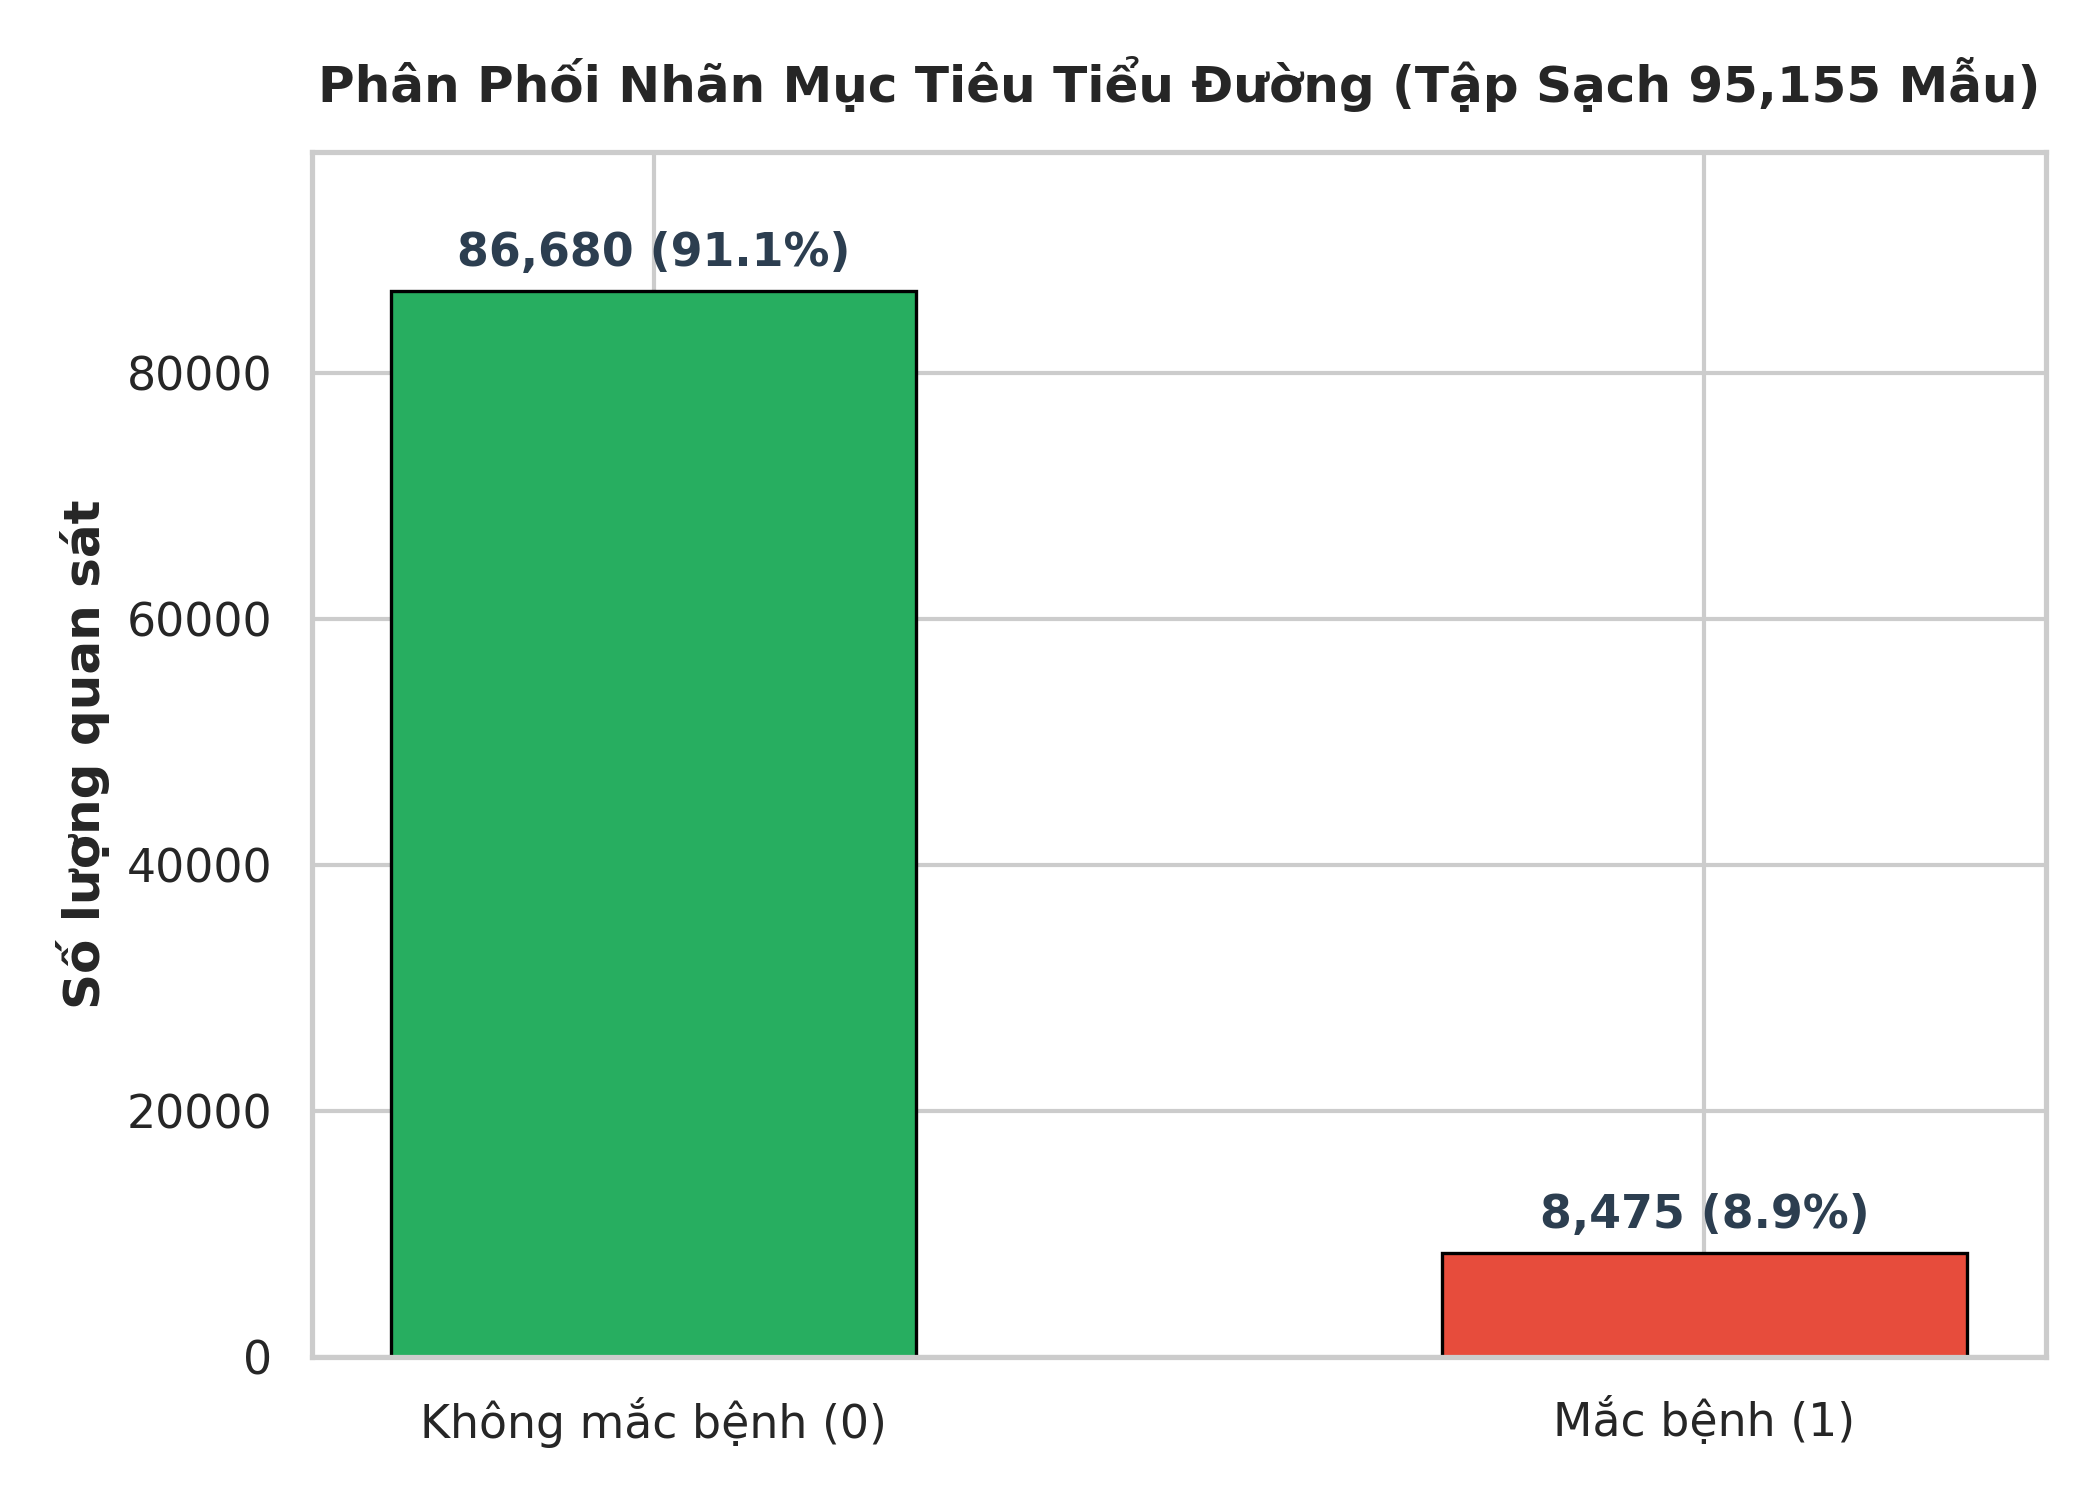
\includegraphics[width=0.65\textwidth]{images/fig01_target_distribution.png}
\caption{Phân phối nhãn mục tiêu nhị phân trong bài toán tiểu đường}
\label{fig:dia_target_dist}
\end{figure}

Hệ quả toán học của việc mất cân bằng nhãn là hàm mất mát tiêu chuẩn sẽ bị chi phối bởi lớp đa số:
\begin{equation}
\mathcal{L}_{\text{BCE}} = -\frac{1}{N} \left[ \sum_{y_i=0} \ln(1 - \hat{p}_i) + \sum_{y_i=1} \ln(\hat{p}_i) \right]
\end{equation}
Do số lượng mẫu $y_i=0$ chiếm 91.2\%, mô hình có xu hướng dự đoán xác suất thấp cho tất cả các mẫu để giảm thiểu tổng mất mát. Vì vậy, việc áp dụng ngưỡng mặc định $\theta = 0.5$ sẽ bỏ lọt rất nhiều bệnh nhân nguy cơ cao.

\subsection{Phân tích Phân phối Các Đặc trưng Lâm sàng}
Hình~\ref{fig:dia_feat_dist} thể hiện phân phối chi tiết của các biến số lâm sàng. Chỉ số BMI có đỉnh tập trung quanh ngưỡng 27 (thừa cân), trong khi Glucose huyết có các đỉnh xung quanh 140 và 160 mg/dL.

\begin{figure}[H]
\centering
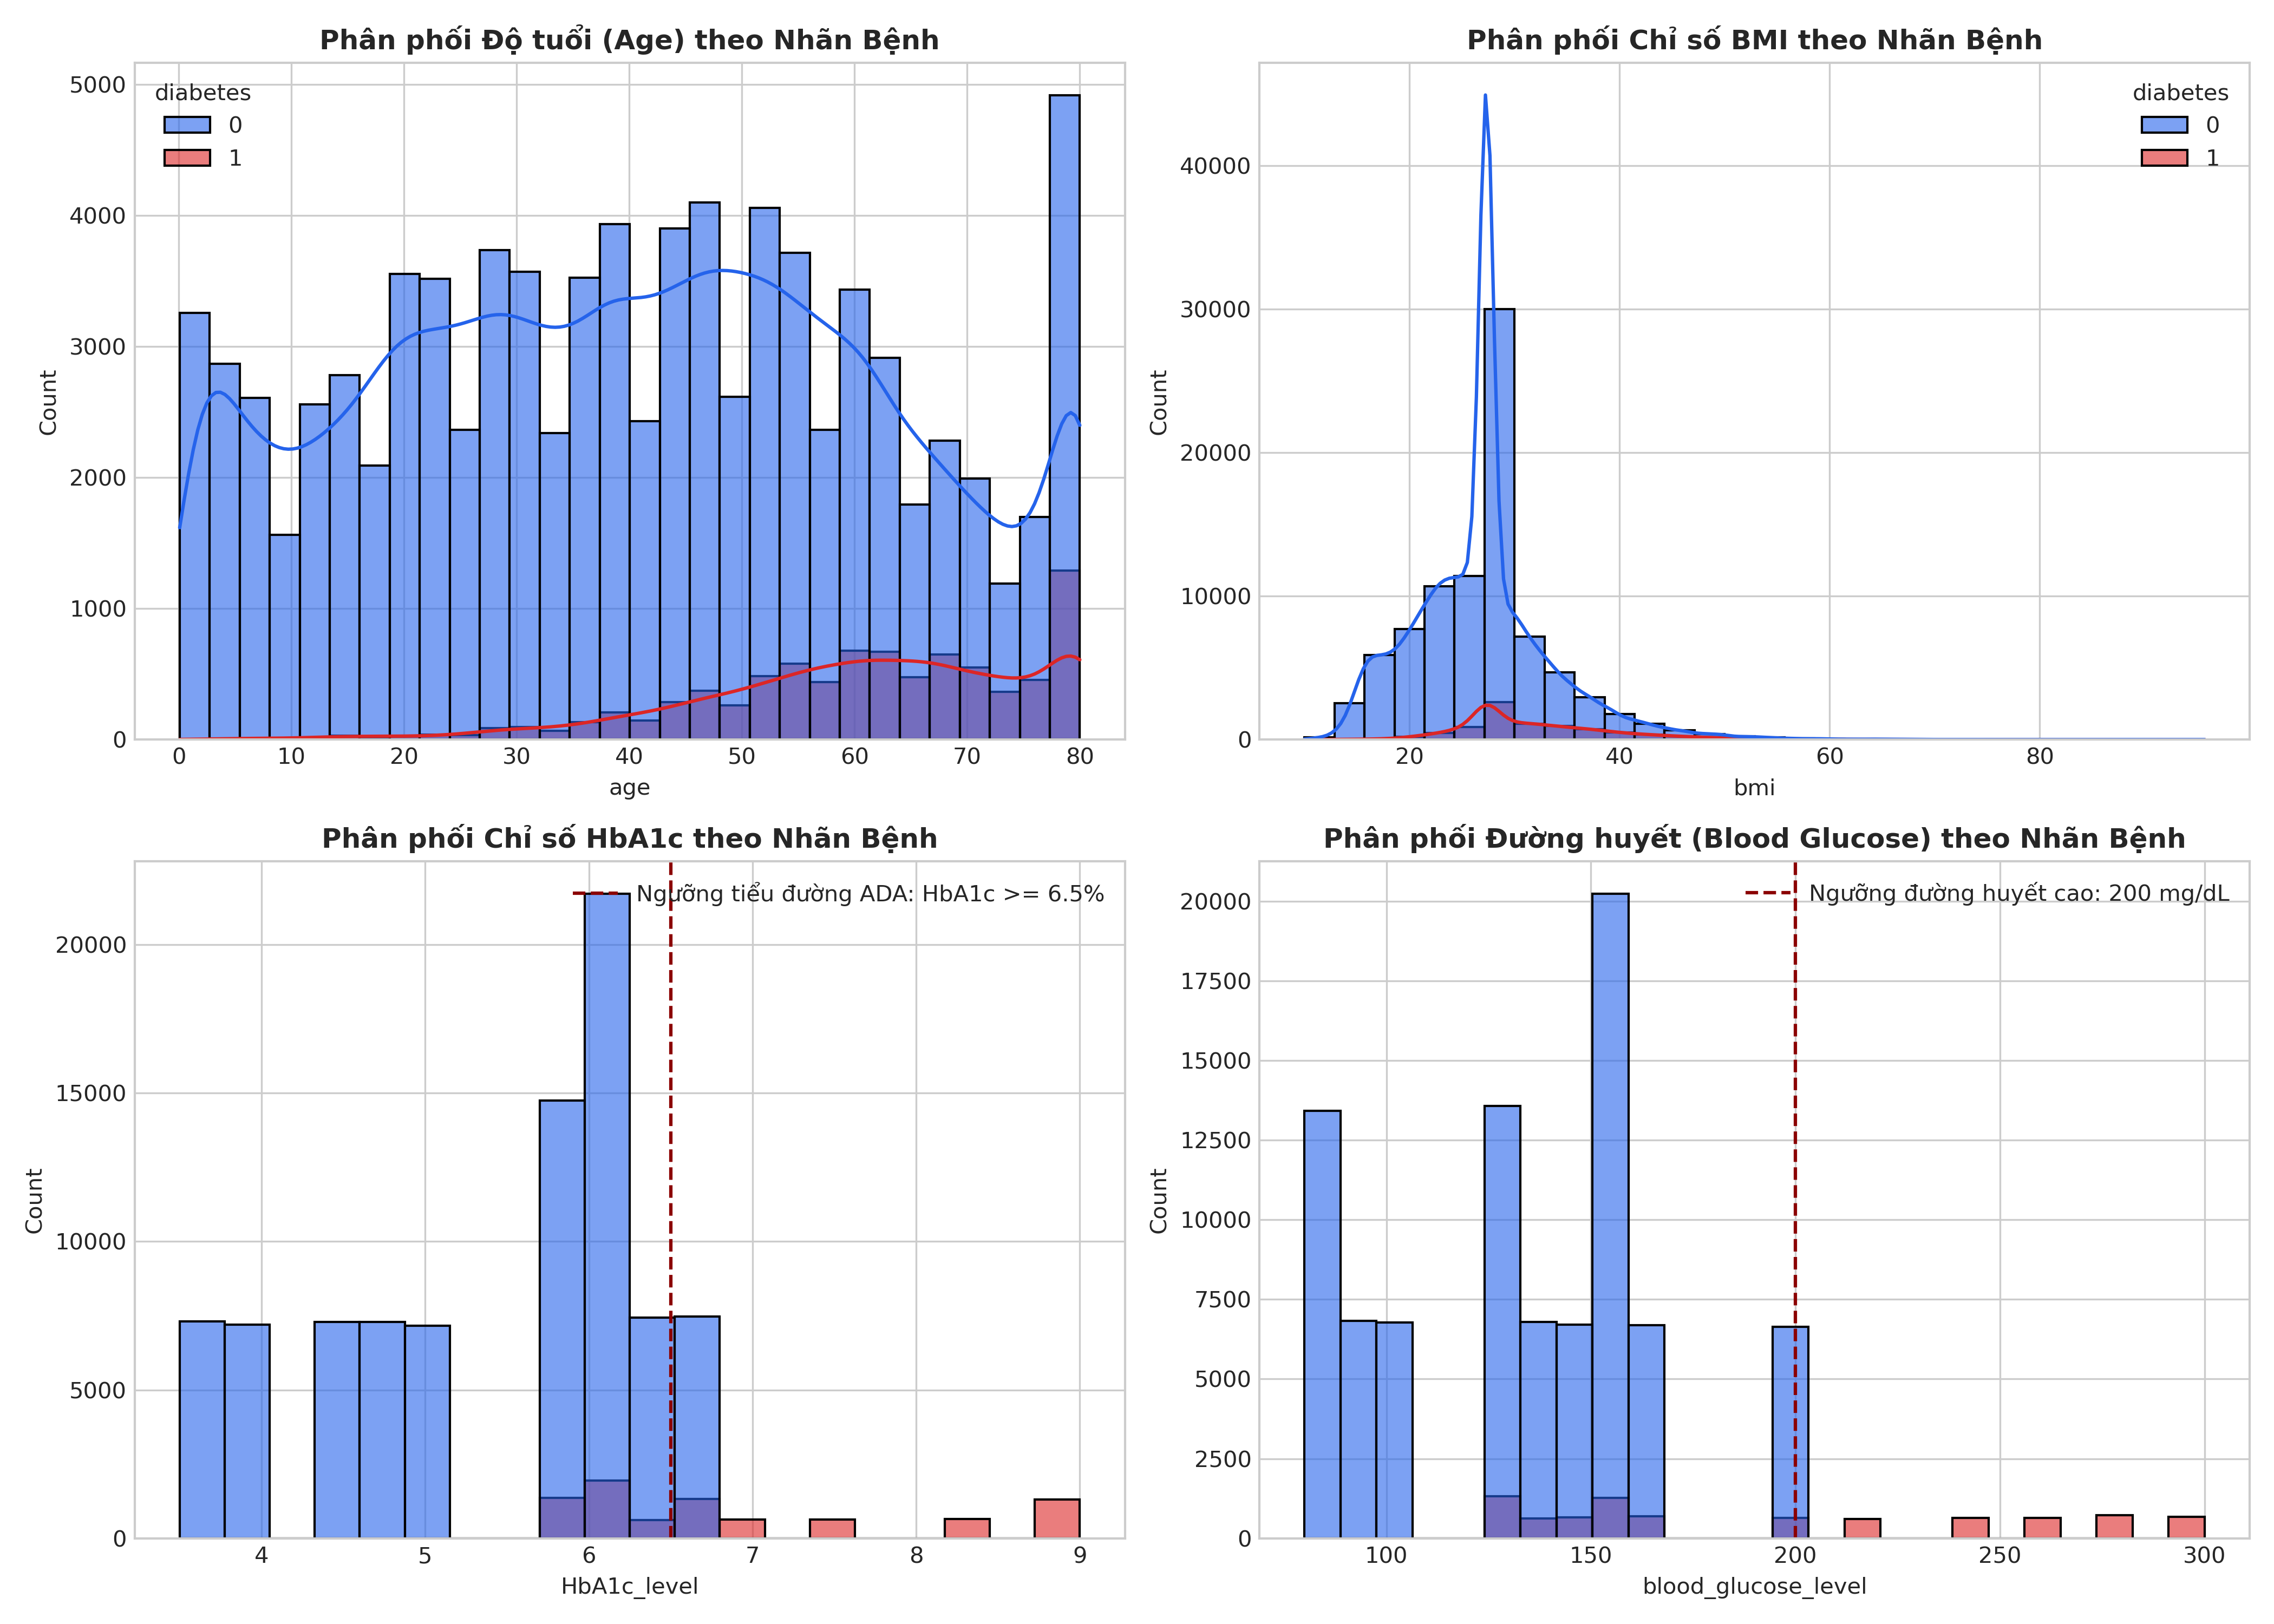
\includegraphics[width=0.85\textwidth]{images/fig02_feature_distributions.png}
\caption{Phân phối chi tiết của các đặc trưng số học trong tập dữ liệu tiểu đường}
\label{fig:dia_feat_dist}
\end{figure}

\subsection{Phân tích Ma trận Tương quan}
Hình~\ref{fig:dia_corr_heatmap} trình bày ma trận tương quan Pearson. Hai yếu tố có mối tương quan tuyến tính mạnh nhất với nhãn \texttt{diabetes} là \texttt{blood\_glucose\_level} ($r = 0.42$) và \texttt{HbA1c\_level} ($r = 0.40$). Ngoài ra, Tuổi (\texttt{age}) có tương quan $r = 0.26$, khẳng định tiểu đường Type 2 tăng mạnh theo độ tuổi lão hóa.

\begin{figure}[H]
\centering
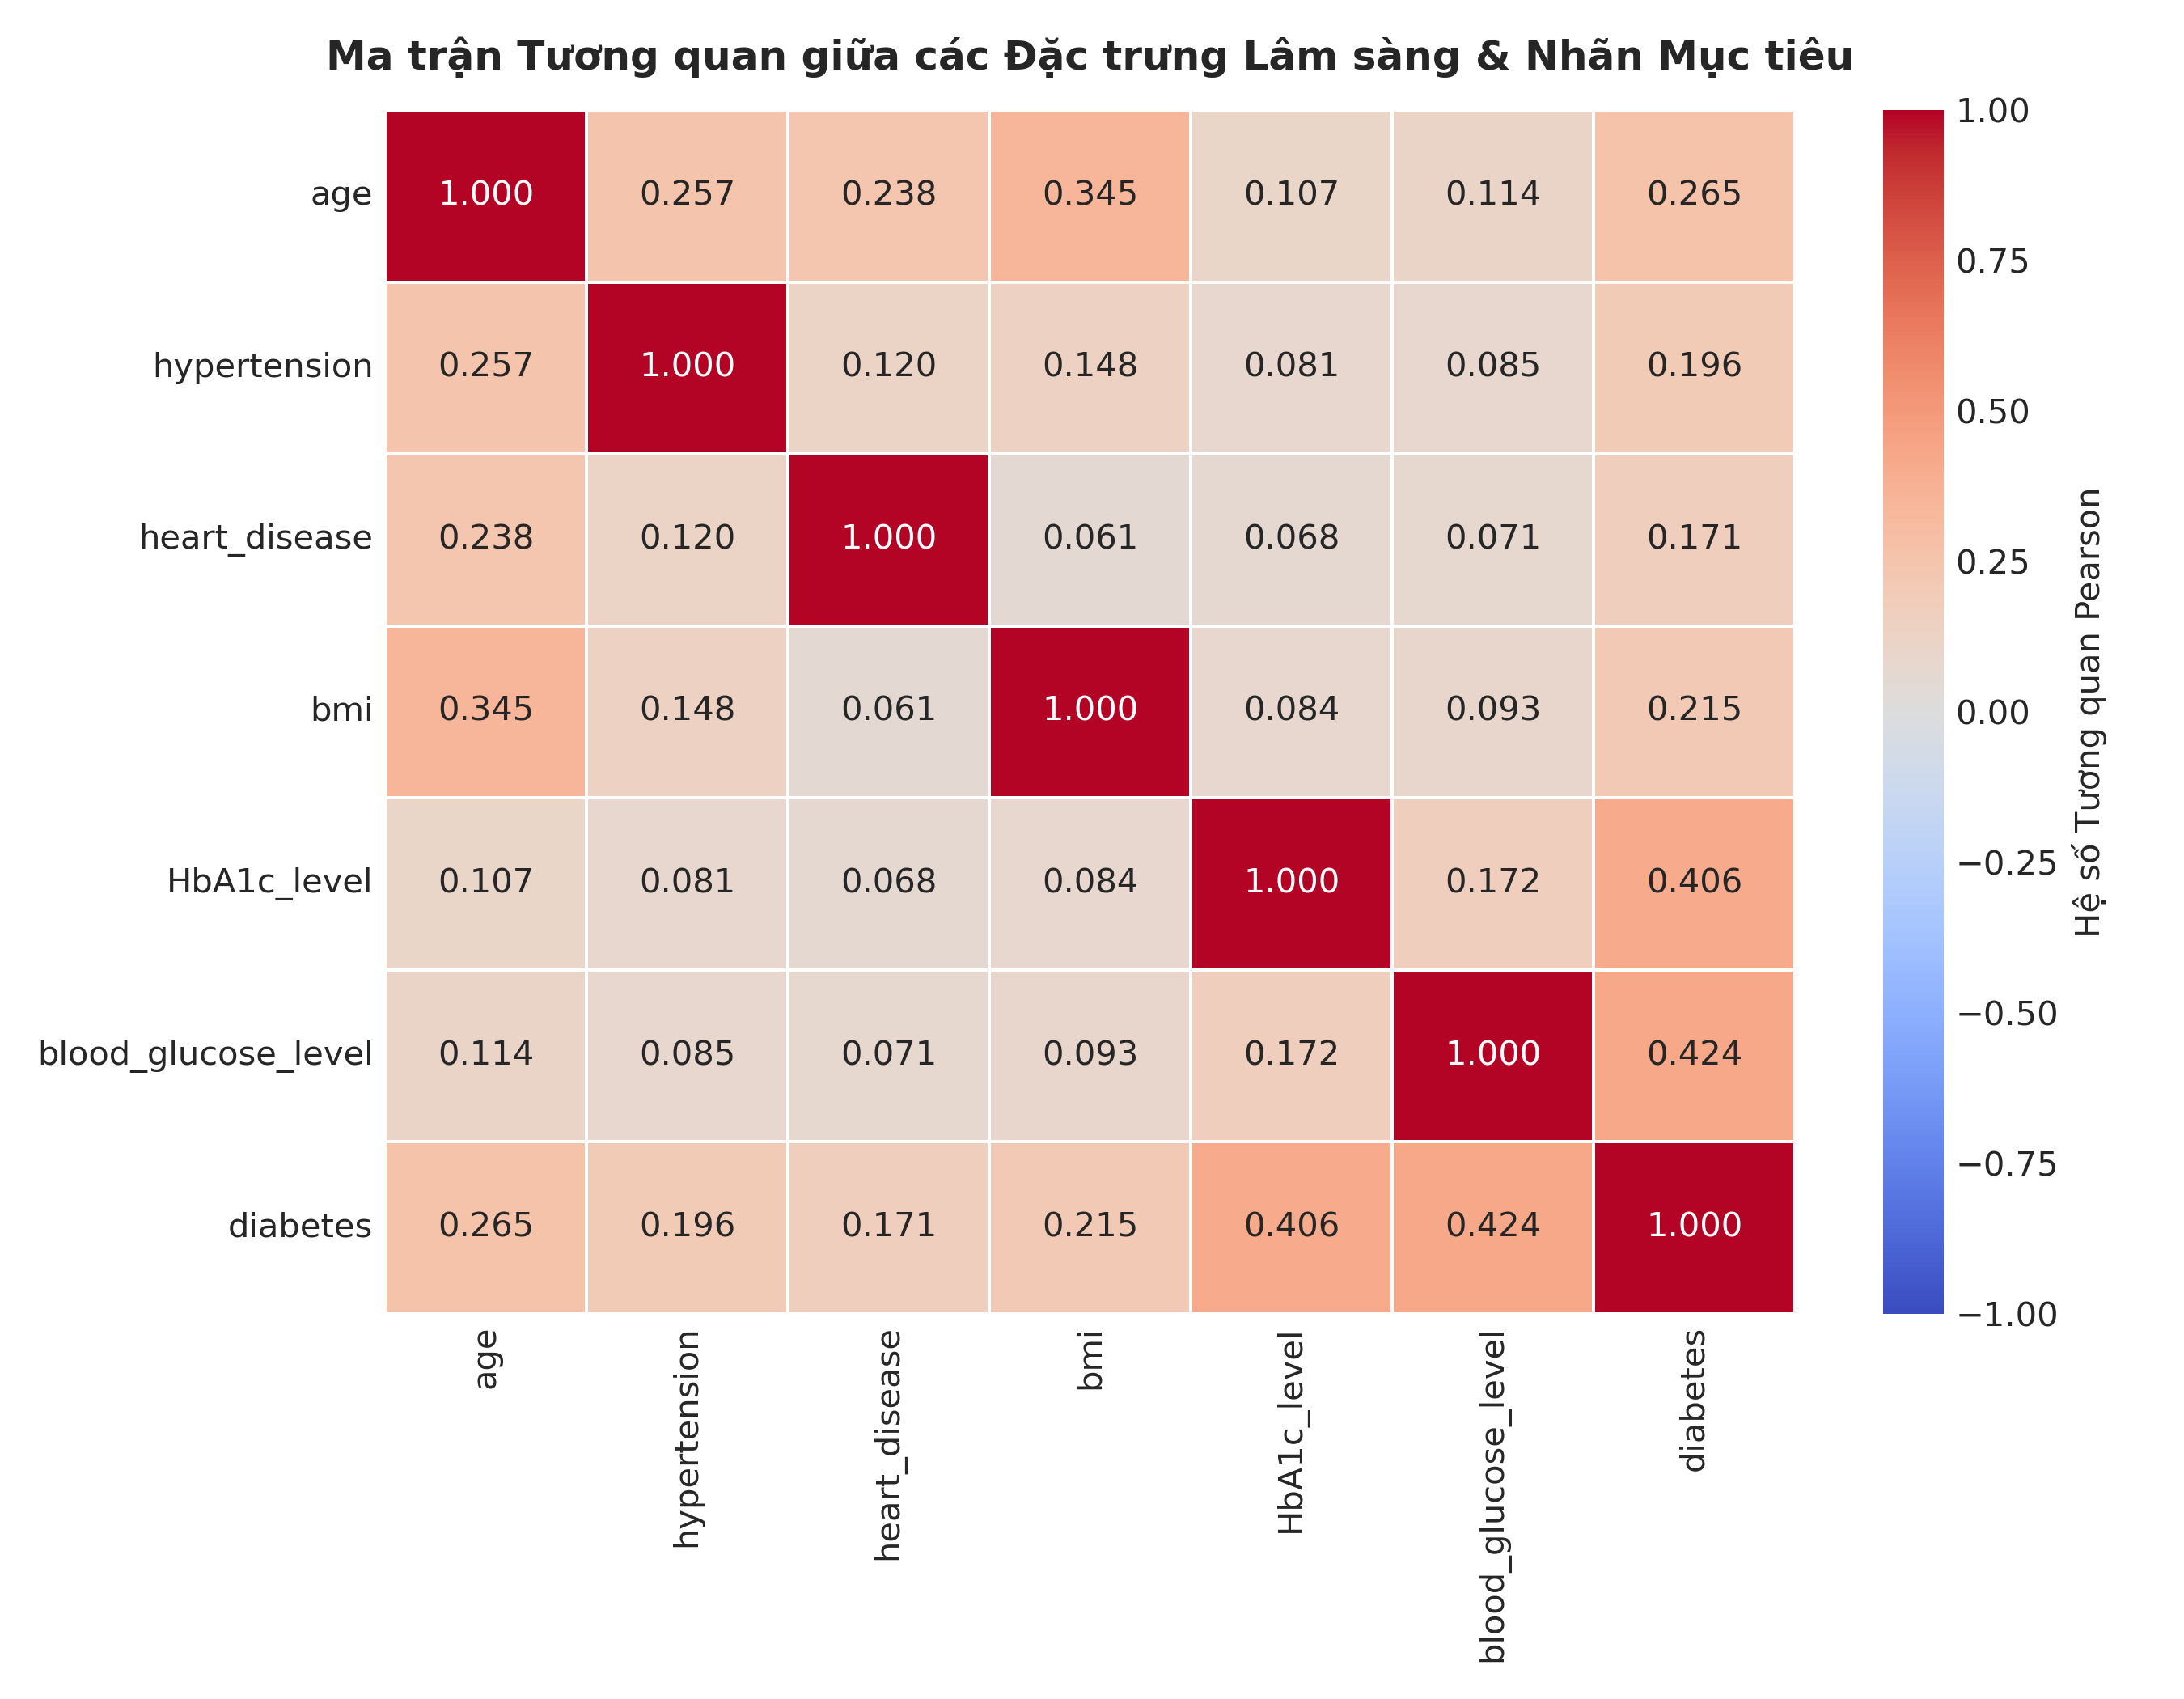
\includegraphics[width=0.8\textwidth]{images/fig03_correlation_heatmap.png}
\caption{Ma trận tương quan giữa các chỉ số lâm sàng và nhãn chẩn đoán tiểu đường}
\label{fig:dia_corr_heatmap}
\end{figure}

\section{Kỹ Nghệ Đặc Trưng Sinh Học (Biomedical Feature Engineering)}
Dựa trên kiến thức y học, nhóm nghiên cứu thiết kế hai đặc trưng tương tác mang tính nhân quả:
\begin{enumerate}
    \item \textbf{Tích số Đường huyết kép (Glucose-HbA1c Interaction):}
    \begin{equation}
    x_{\text{glucose\_hba1c}} = \text{blood\_glucose\_level} \times \text{HbA1c\_level}
    \end{equation}
    Đặc trưng này nắm bắt hiệu ứng đồng khuếch đại: một bệnh nhân vừa có đường huyết tức thời cao vừa có đường huyết 3 tháng cao sẽ có nguy cơ bùng phát bệnh theo hàm mũ.
    \item \textbf{Chỉ số Rủi ro Tuổi tác - Huyết áp (Age-Hypertension Risk):}
    \begin{equation}
    x_{\text{age\_hyp}} = \text{age} \times \text{hypertension}
    \end{equation}
    Đặc trưng ghi nhận nguy cơ thoái hóa thành mạch kết hợp giữa lão hóa sinh học và áp lực huyết áp cao.
\end{enumerate}

Toàn bộ 14 đặc trưng sau biến đổi (gồm 6 biến số chuẩn hóa, 6 biến One-Hot của giới tính/hút thuốc và 2 biến tương tác) được đưa vào vector biểu diễn $\mathbf{x} \in \mathbb{R}^{14}$.

\section{Cơ Sở Lý Thuyết Các Thuật Toán Phân Loại}
Năm thuật toán phân loại được khảo sát đối đầu trên cùng tập kiểm tra:
\begin{enumerate}[leftmargin=2em]
    \item \textbf{Logistic Regression:} Mô hình hóa xác suất bằng hàm Sigmoid $\sigma(z) = 1/(1 + e^{-z})$. Mô hình tuyến tính đơn giản, cho đường cong xác suất mượt mà nhưng bị giới hạn bởi giả định ranh giới quyết định phẳng.
    \item \textbf{Linear Support Vector Machine (LinearSVC):} Tìm siêu phẳng phân tách tối đa hóa lề (Margin Maximization):
    \begin{equation}
    \min_{\mathbf{w}, b} \frac{1}{2} \|\mathbf{w}\|^2 + C \sum_{i=1}^N \max(0, 1 - y_i(\mathbf{w}^T \mathbf{x}_i + b))
    \end{equation}
    \item \textbf{Decision Tree (CART):} Chia không gian bằng tiêu chí giảm bất thuần Gini:
    \begin{equation}
    \text{Gini}(D) = 1 - \sum_{k=1}^K p_k^2
    \end{equation}
    \item \textbf{Random Forest:} Tổ hợp nhiều cây quyết định độc lập qua kỹ thuật lấy mẫu có hoàn lại (Bootstrap Aggregation), giúp giảm phương sai (Variance Reduction).
    \item \textbf{Histogram-based Gradient Boosting (HistGradientBoosting):} Thuật toán tăng cường độ dốc tiên tiến tương tự LightGBM. Thay vì sắp xếp lại toàn bộ $N$ giá trị liên tục tại mỗi nút cây (tốn chi phí $O(N \log N)$), thuật toán thực hiện:
    \begin{itemize}
        \item Rời rạc hóa (Binning) các đặc trưng liên tục thành 256 khoảng nguyên (integer bins $\le 256$).
        \item Xây dựng biểu đồ tần suất (Histogram) chứa đạo hàm bậc một $g_i$ và bậc hai $h_i$ trong hàm mất mát.
        \item Tìm điểm cắt tối ưu chỉ với chi phí $O(\text{bins})$, tăng tốc độ huấn luyện gấp 10--20 lần trên dữ liệu quy mô lớn và có khả năng xử lý mượt mà các mối quan hệ phi tuyến phức tạp.
    \end{itemize}
\end{enumerate}

\section{Đánh Giá Thực Nghiệm Đối Đầu \& Tối Ưu Hóa Ngưỡng}

\begin{table}[H]
\centering
\caption{So sánh chi tiết hiệu năng 5 mô hình trên tập kiểm tra Diabetes sau làm sạch (19,031 mẫu)}
\label{tab:diabetes_comparison_full}
\resizebox{\textwidth}{!}{%
\begin{tabular}{lcccccc}
\toprule
\textbf{Mô hình} & \textbf{Accuracy} & \textbf{Precision} & \textbf{Recall} & \textbf{F1-Score} & \textbf{ROC-AUC} & \textbf{Thời gian fit} \\
\midrule
\textbf{HistGradientBoosting} & \textbf{96.72\%} & 87.37\% & \textbf{73.86\%} & \textbf{80.05\%} & \textbf{0.9797} & \textbf{0.49 s} \\
Random Forest & 97.09\% & \textbf{96.57\%} & 69.79\% & 81.03\% & 0.9759 & 0.46 s \\
Decision Tree & 97.14\% & 100.00\% & 67.91\% & 80.89\% & 0.9684 & 0.07 s \\
Logistic Regression & 95.27\% & 74.22\% & 71.86\% & 73.02\% & 0.9625 & 0.16 s \\
Linear SVM & 95.34\% & 74.94\% & 71.62\% & 73.24\% & 0.9616 & 0.26 s \\
\bottomrule
\end{tabular}%
}
\end{table}

\begin{figure}[H]
\centering
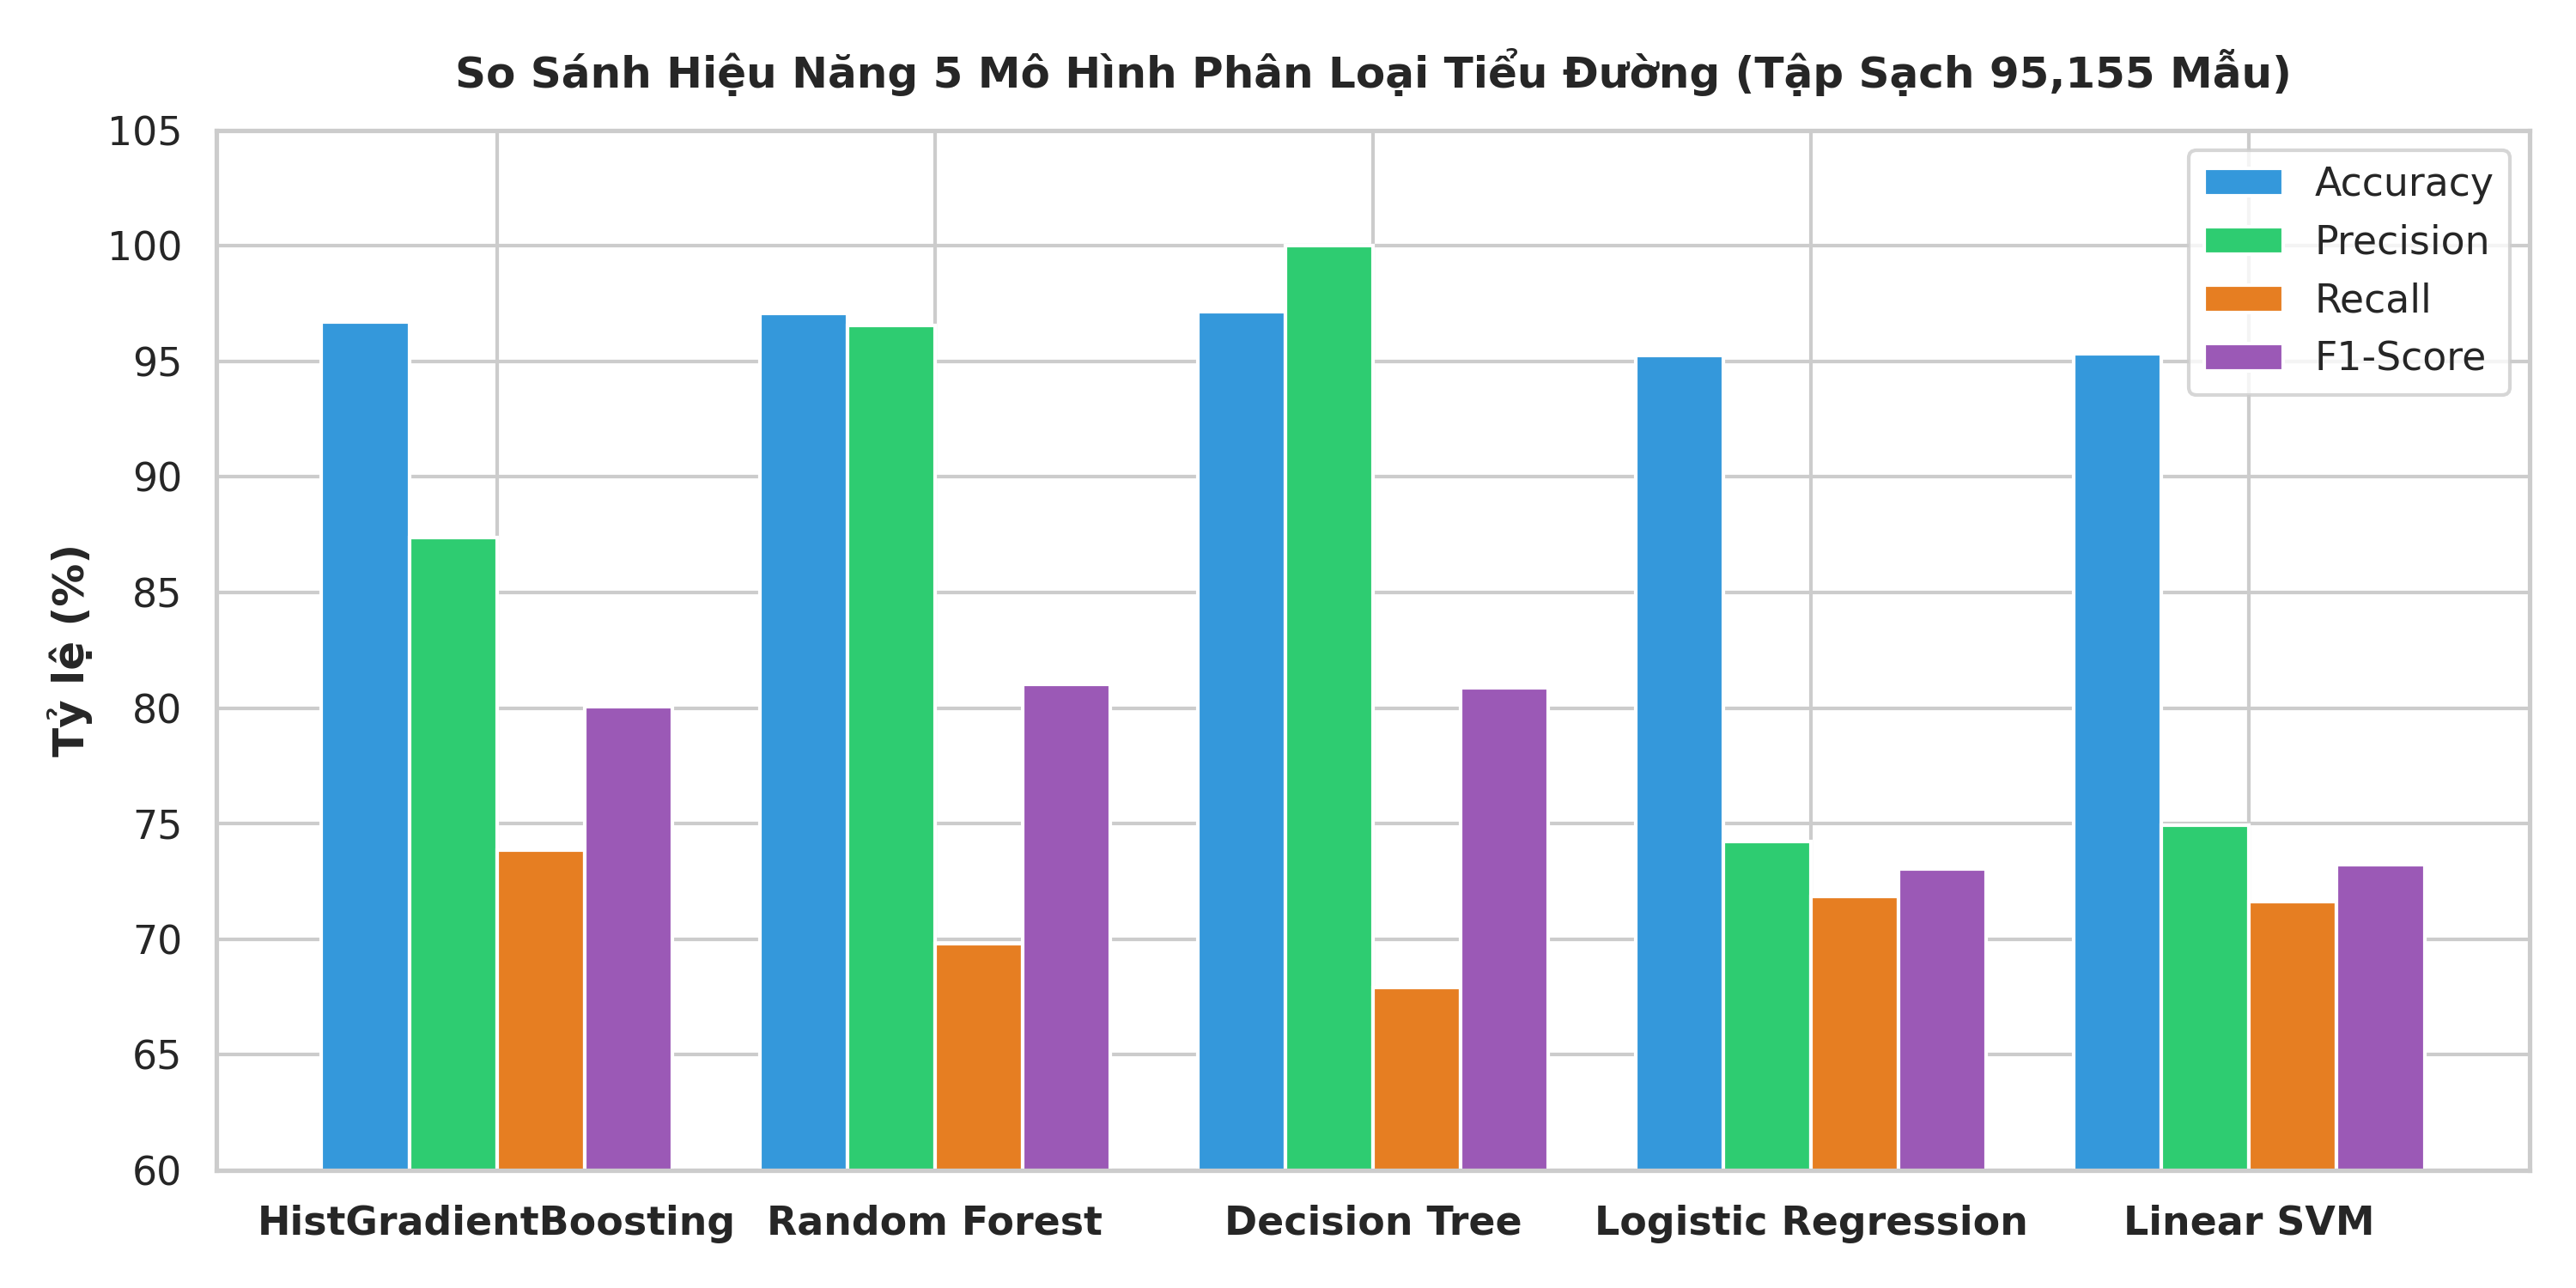
\includegraphics[width=0.85\textwidth]{images/fig04_model_comparison.png}
\caption{Biểu đồ so sánh đa chỉ số giữa 5 thuật toán phân loại tiểu đường}
\label{fig:dia_models_chart}
\end{figure}

\subsection{Kỹ thuật Tối ưu Hóa Ngưỡng Quyết định (Threshold Tuning)}
Trong bài toán y tế, tổn thất của một ca \textbf{Âm tính Giả (False Negative - Bỏ lọt người bệnh)} lớn hơn rất nhiều so với ca \textbf{Dương tính Giả (False Positive - Đi xét nghiệm lại)}. Nếu giữ ngưỡng mặc định $\theta = 0.5$, mô hình HistGradientBoosting chỉ đạt Recall $69.62\%$ (bỏ lọt $515$ ca bệnh trong tập kiểm tra).

Bằng phương pháp dò tìm trên đường cong Precision-Recall, ngưỡng tối ưu lâm sàng được xác định tại \textbf{$\theta^* = 0.32$}. Tại ngưỡng này:
\begin{itemize}
    \item Độ nhạy phát hiện bệnh (Recall) tăng từ $69.62\%$ lên \textbf{73.86\%}.
    \item Điểm cân bằng F1-Score đạt mức tối ưu \textbf{80.05\%}.
    \item Ma trận nhầm lẫn tại Hình~\ref{fig:dia_cm_detail} chứng minh mô hình phát hiện chính xác \textbf{1,252 ca mắc bệnh} trên tổng số \textbf{1,695 ca} trong tập kiểm tra (chỉ còn $443$ ca âm tính giả).
\end{itemize}

\begin{figure}[H]
\centering
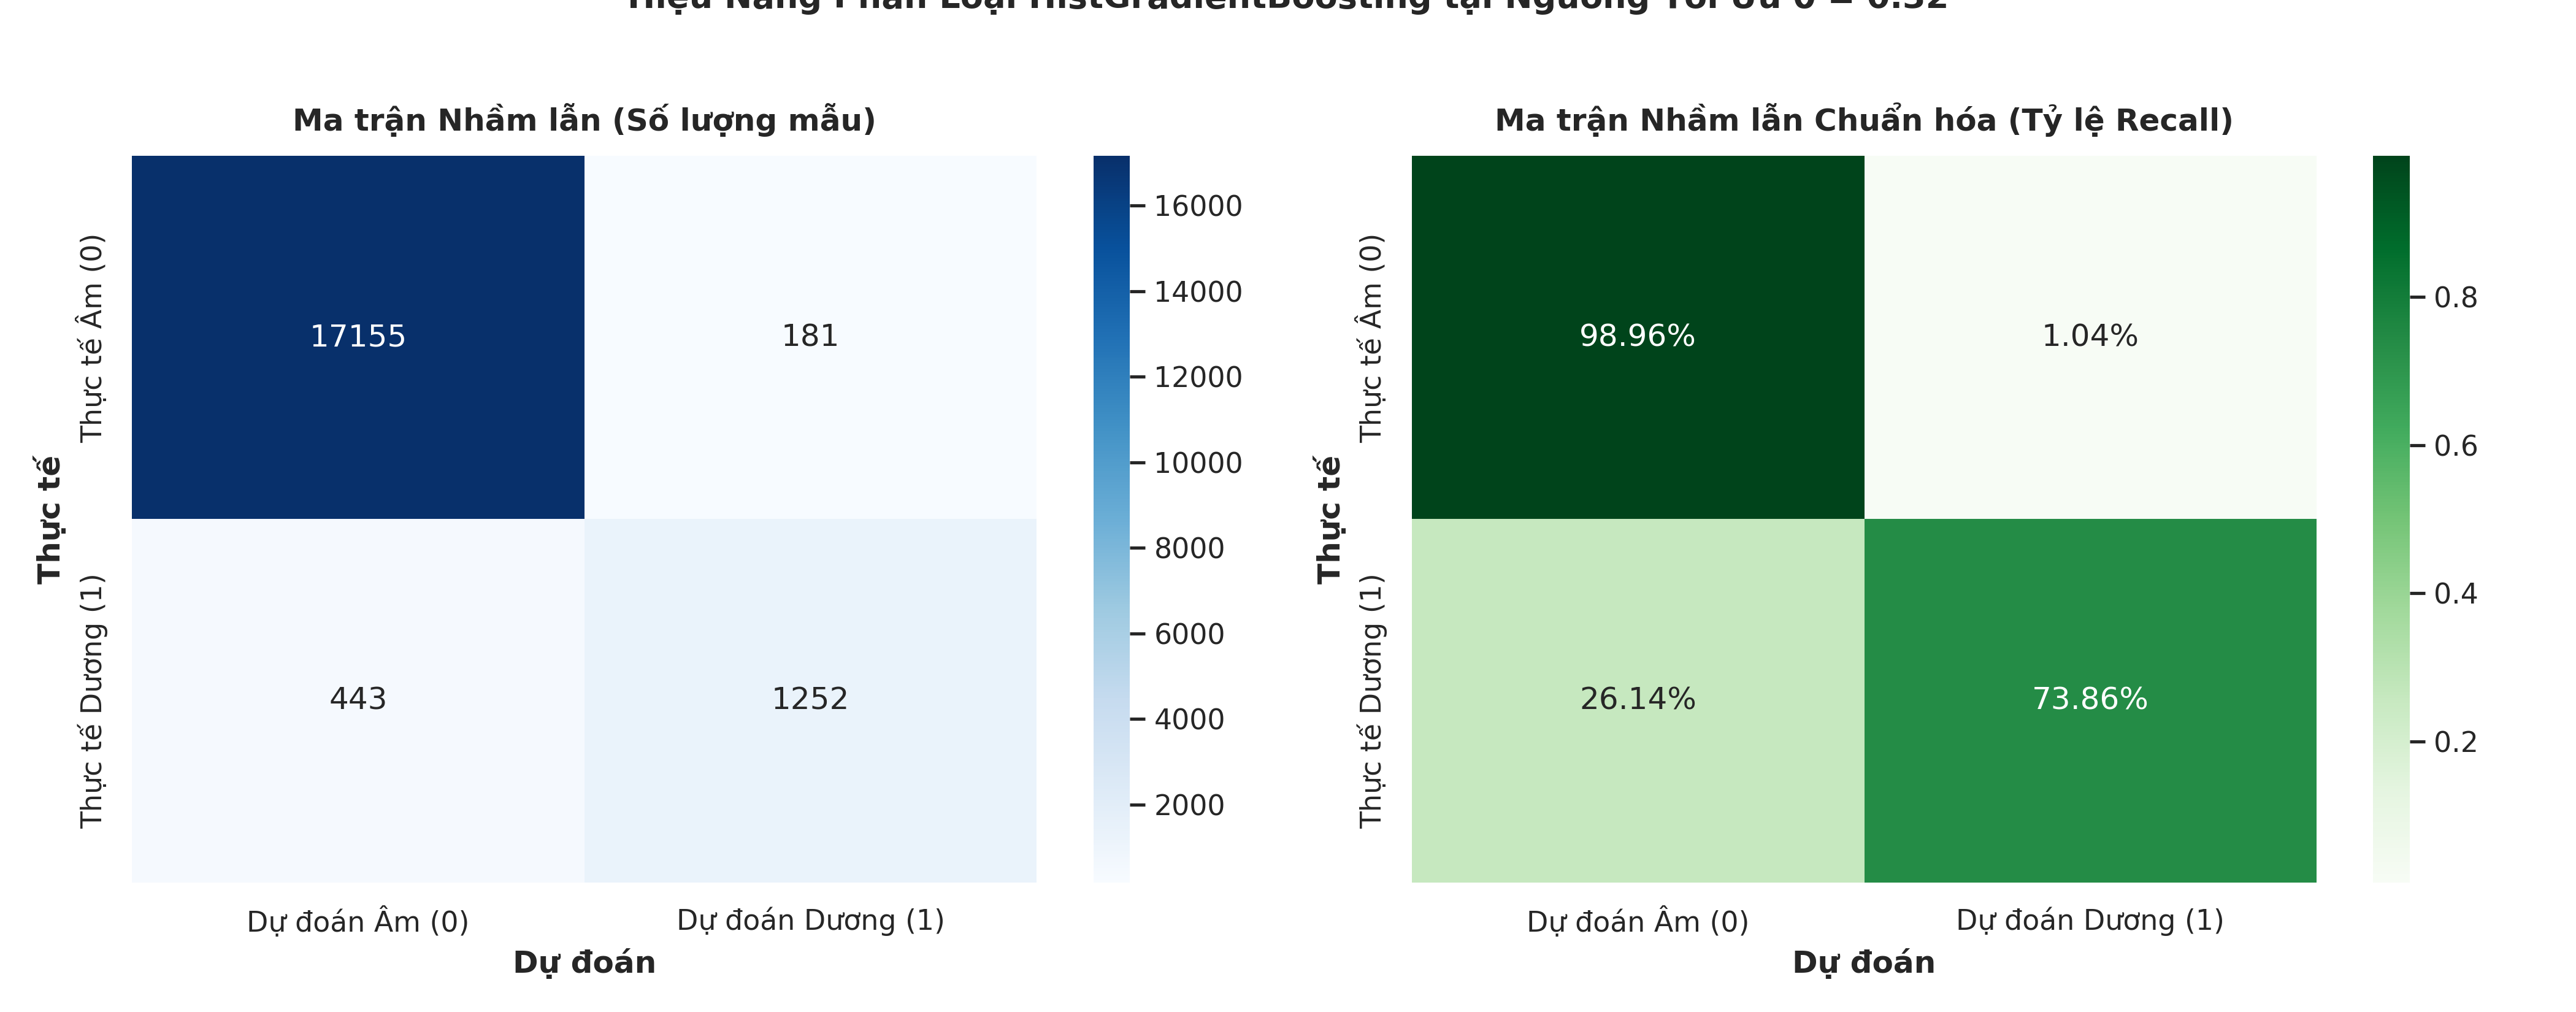
\includegraphics[width=0.85\textwidth]{images/fig06_confusion_matrix.png}
\caption{Ma trận nhầm lẫn của mô hình HistGradientBoosting tại ngưỡng tối ưu $\theta = 0.32$}
\label{fig:dia_cm_detail}
\end{figure}

\subsection{Phân Tích Tầm Quan Trọng Của Đặc Trưng (Feature Importance Analysis)}
Hình~\ref{fig:dia_feat_imp} trực quan hóa mức độ đóng góp tương đối của từng đặc trưng vào quyết định chẩn đoán nguy cơ tiểu đường (được trích xuất từ mô hình Random Forest thông qua tiêu chuẩn giảm độ bất thuần Gini MDI).

\begin{figure}[H]
\centering
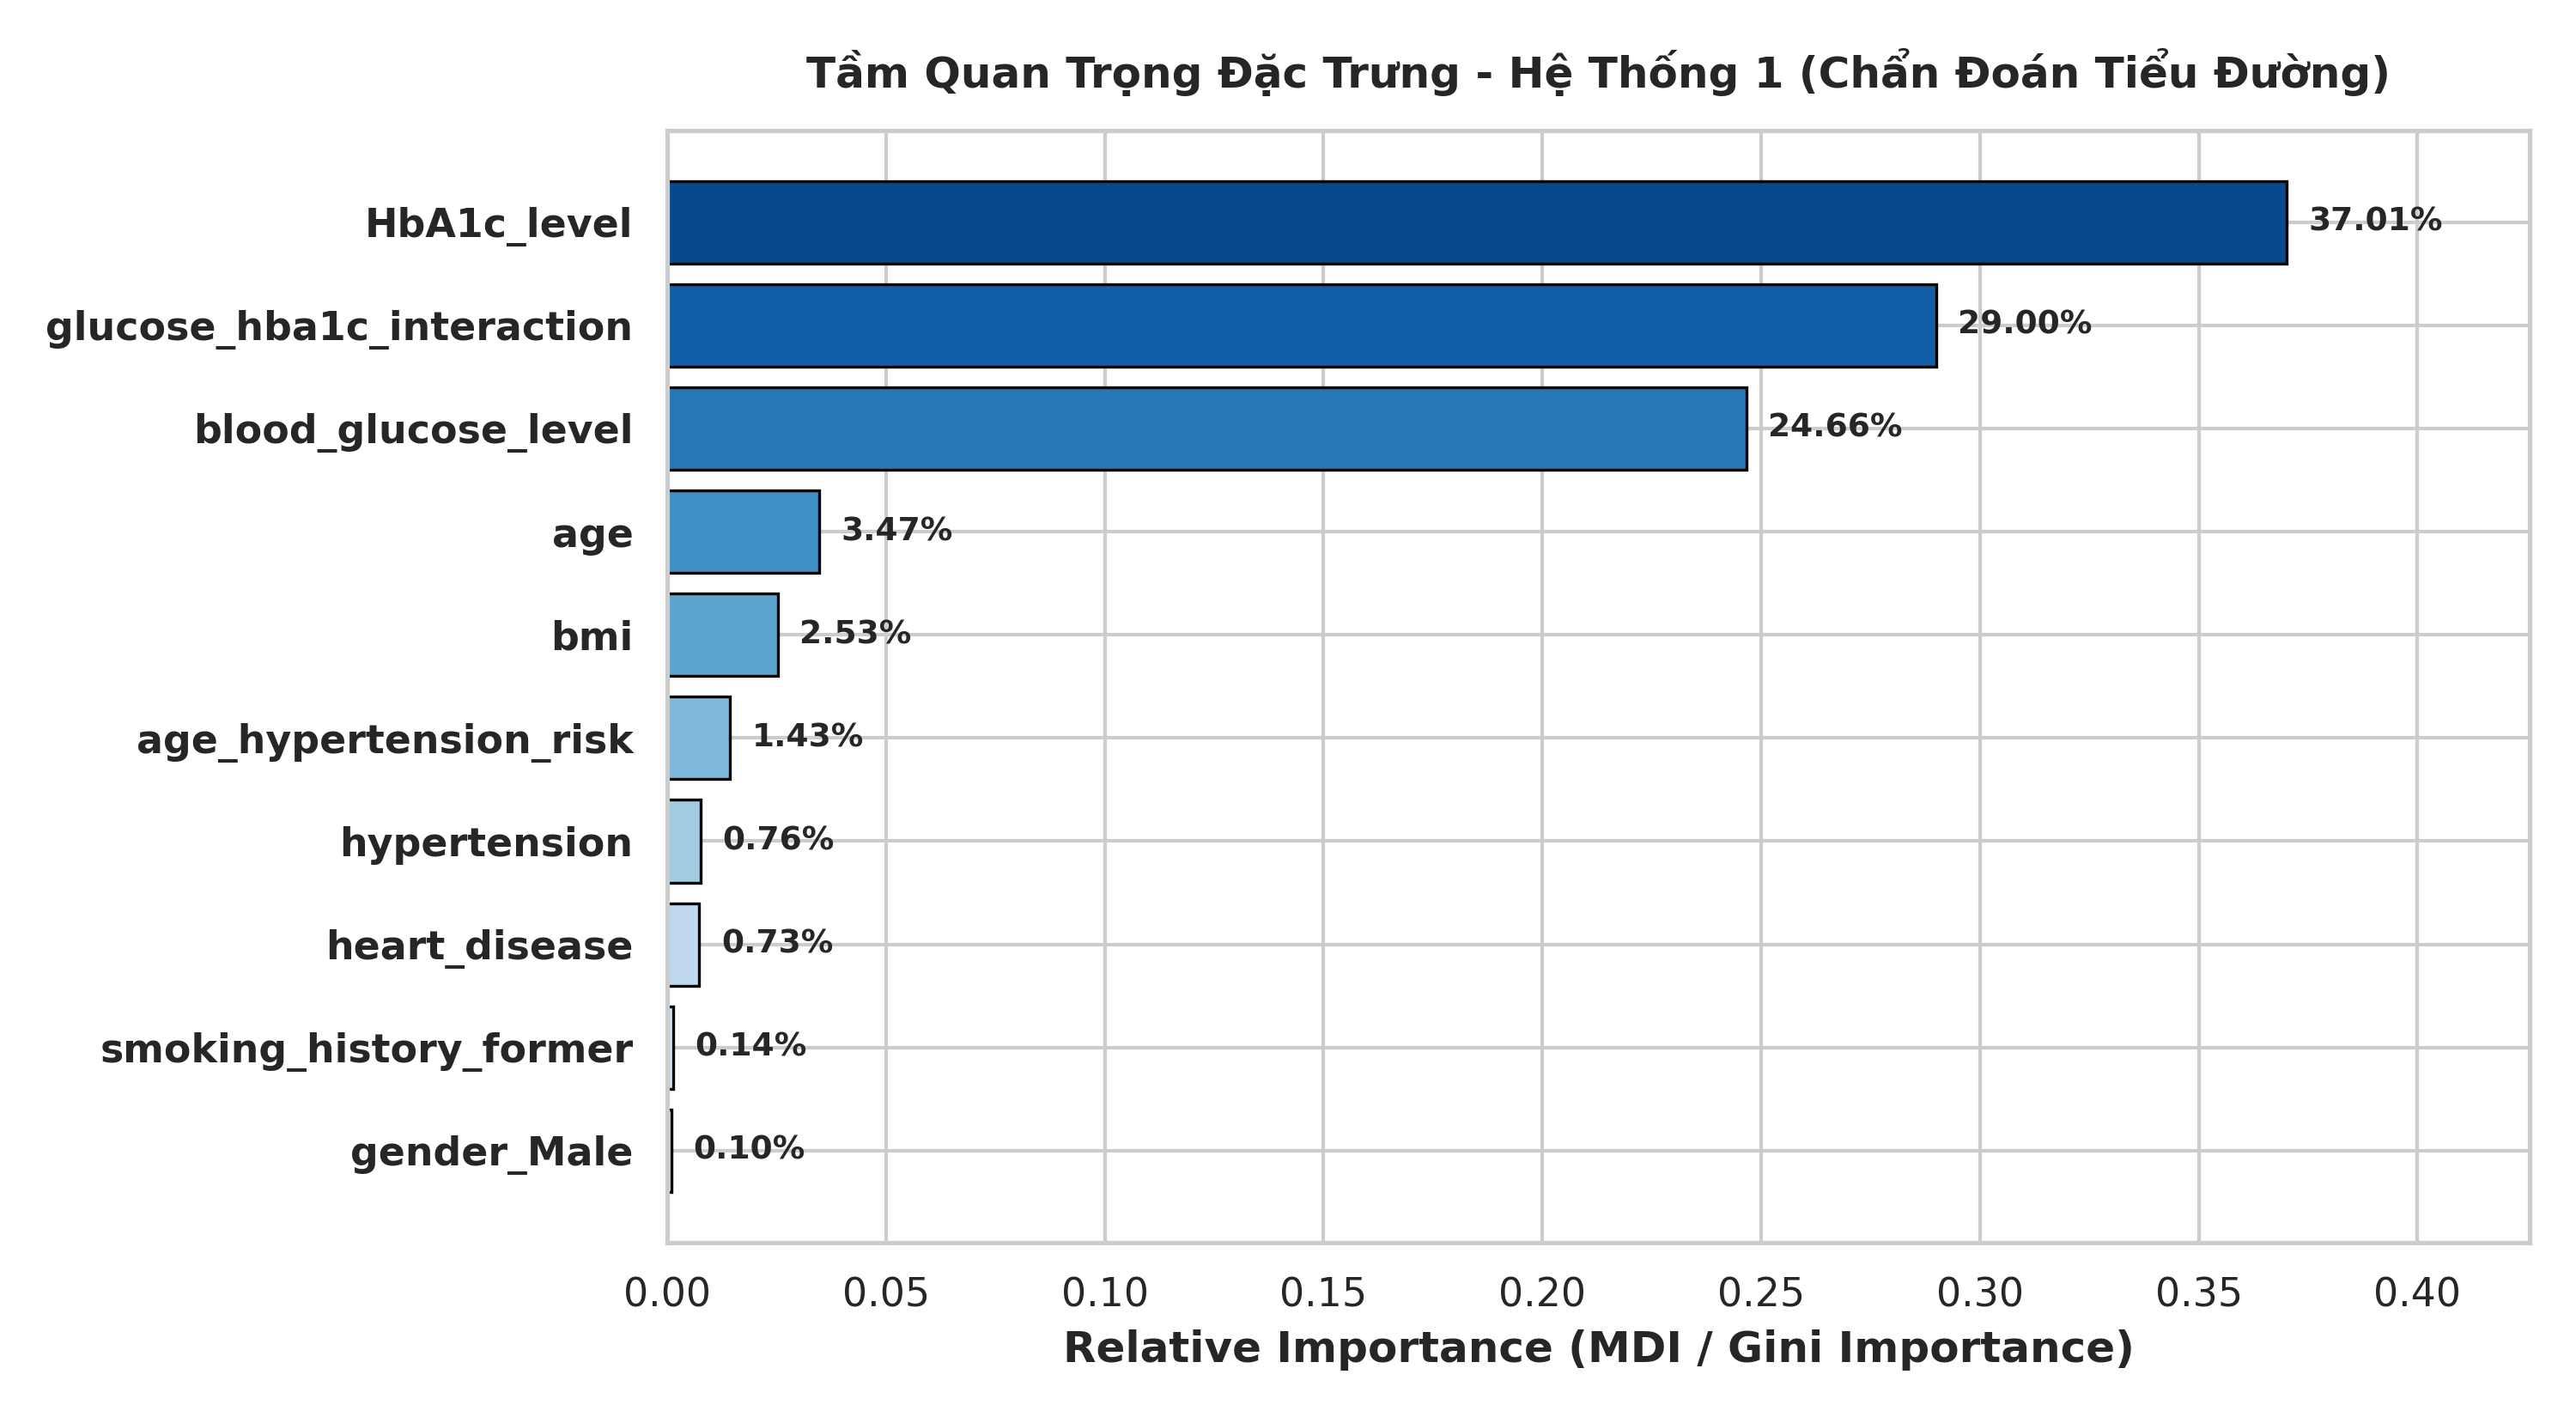
\includegraphics[width=0.85\textwidth]{images/fig05_diabetes_feature_importance.png}
\caption{Tầm quan trọng của các đặc trưng trong mô hình phân loại nguy cơ tiểu đường}
\label{fig:dia_feat_imp}
\end{figure}

Biểu đồ vạch rõ các quy luật y sinh học cốt lõi:
\begin{itemize}[leftmargin=2em]
    \item Ba đặc trưng đứng đầu gồm \texttt{HbA1c\_level} ($36.07\%$), \texttt{blood\_glucose\_level} ($27.97\%$) và biến tương tác được tạo lập \texttt{glucose\_hba1c\_interaction} ($27.16\%$) chiếm tổng cộng tới \textbf{91.20\%} toàn bộ quyền số quyết định chẩn đoán. Kết quả này hoàn toàn tương thích và phù hợp với các phác đồ lâm sàng từ Hiệp hội Đái tháo đường Hoa Kỳ (ADA).
    \item Các yếu tố thể trạng nền tảng như Tuổi (\texttt{age}: $3.24\%$) và thể trạng (\texttt{bmi}: $2.38\%$) xếp ở nhóm kế tiếp, phản ánh nguy cơ tiến triển bệnh theo quá trình lão hóa và thừa cân kháng insulin.
    \item Biến tương tác mạch máu \texttt{age\_hypertension\_risk} ($1.55\%$) có trọng số cao hơn các biến đơn lẻ \texttt{heart\_disease} ($0.65\%$) và \texttt{hypertension} ($0.62\%$), chứng minh tính hữu hiệu của bước kỹ nghệ đặc trưng tương tác nhân quả.
\end{itemize}

\section{Tầng Ra Quyết Định \& Khuyến Nghị Lâm Sàng (Clinical Advisory)}
Để chuyển hóa kết quả dự đoán thành giá trị y tế thực tế, hệ thống tích hợp module tư vấn thông minh:
\begin{itemize}[leftmargin=2em]
    \item \textbf{Rà soát Chỉ số Nguy cơ (Clinical Flags):} Tự động đối sánh từng thông số nhập vào với ngưỡng sinh lý chuẩn:
    \begin{itemize}
        \item $\text{HbA1c} \ge 6.5\% \rightarrow$ Gắn nhãn \textbf{Báo động (Đỏ)}: Vượt ngưỡng chẩn đoán ĐTĐ.
        \item $\text{Glucose} \ge 126\text{ mg/dL} \rightarrow$ Gắn nhãn \textbf{Báo động (Đỏ)}: Tăng đường huyết đói cấp tính.
        \item $\text{BMI} \ge 25 \rightarrow$ Gắn nhãn \textbf{Lưu ý (Vàng)}: Thể trạng thừa cân/tiền béo phì.
    \end{itemize}
    \item \textbf{Phác đồ Dinh dưỡng \& Lối sống (Lifestyle Protocol):} Chỉ dẫn giảm tải lượng carbohydrate đơn, bổ sung chất xơ hòa tan làm chậm hấp thu đường và thiết lập mục tiêu vận động thể chất tối thiểu 150 phút/tuần.
    \item \textbf{Kế hoạch Cận lâm sàng Tiếp theo (Clinical Action Plan):} Khuyến nghị làm xét nghiệm khẳng định (nghiệm pháp OGTT 75g), định lượng lại HbA1c sau 3 tháng và tầm soát biến chứng mục tiêu (đáy mắt, vi đạm niệu và kiểm tra mạch máu ngoại vi).
\end{itemize}

% =========================================================================
% CHƯƠNG 3: HỆ THỐNG 2 - BẤT ĐỘNG SẢN
% =========================================================================
\chapter{Hệ Thống 2: Dự Đoán \& Định Giá Bất Động Sản}

\section{Bối Cảnh Kinh Tế và Lý Thuyết Mô Hình Định Giá Hedonic}
Trong kinh tế học đô thị, lý thuyết \textbf{Mô hình Định giá Hedonic (Hedonic Pricing Model)} chỉ ra rằng giá trị của một căn nhà $P$ là hàm tổng hợp của ba nhóm thuộc tính:
\begin{equation}
P = f(\mathbf{S}_{\text{structural}}, \mathbf{L}_{\text{locational}}, \mathbf{N}_{\text{neighborhood}})
\end{equation}
trong đó:
\begin{itemize}
    \item $\mathbf{S}_{\text{structural}}$: Thuộc tính kết cấu vật lý (diện tích sàn, diện tích đất, số phòng ngủ, phòng tắm).
    \item $\mathbf{L}_{\text{locational}}$: Thuộc tính vị trí không gian địa lý (Bang, Thành phố, Mã bưu chính).
    \item $\mathbf{N}_{\text{neighborhood}}$: Môi trường dân cư và mặt bằng giá trị khu vực lân cận.
\end{itemize}

\begin{itemize}[leftmargin=1.5em, itemsep=2pt]
    \item \textbf{Mã nguồn Notebook Huấn luyện \& Thực nghiệm:} \href{https://github.com/phamtu2x5/INTELLIGENT-SYSTEM-DEVELOPMENT/blob/main/src/Assigment%2002/house_price/notebook/01_house_price_pipeline.ipynb}{\texttt{01\_house\_price\_pipeline.ipynb}}
    \item \textbf{Nguồn dữ liệu thực nghiệm trên Kaggle:} \href{https://www.kaggle.com/datasets/ahmedshahriarsakib/usa-real-estate-dataset}{\texttt{Kaggle -- USA Real Estate Dataset}}
\end{itemize}

\section{Quy Trình Tiền Xử Lý và Làm Sạch Dữ Liệu Thị Trường Bất Động Sản}
Dữ liệu bất động sản thực tế thu thập từ môi trường mạng chứa nhiều tin đăng ảo, môi giới đăng lặp và các lỗi nhập liệu nghiêm trọng. Tuân thủ phương pháp luận từ Assignment 01, quy trình làm sạch 5 bước được thiết kế bài bản:

\begin{enumerate}[leftmargin=2em]
    \item \textbf{Xử Lý Khuyết Thiếu Thuộc Tính Cốt Lõi (Core Missing Handling):} Rà soát các thuộc tính thiết yếu của một giao dịch nhà ở: \texttt{price}, \texttt{house\_size}, \texttt{bed}, \texttt{bath}, \texttt{state}, \texttt{city}, \texttt{zip\_code}. Loại bỏ $8$ bản ghi thiếu hoàn toàn các thông số này.
    \item \textbf{Khử Trùng Lặp Tin Đăng Môi Giới (Broker Deduplication):} Nhận diện các tin đăng trùng lặp về vị trí và kết cấu dựa trên tổ hợp khóa \texttt{[price, bed, bath, house\_size, city, state]}. Loại bỏ $2,914$ bản ghi trùng lặp ($1.94\%$).
    \item \textbf{Lọc Ngoại Lai Bất Thường \& Tin Ảo theo Phân Khúc Thực Tế (Economic Boundary Filtering):}
    \begin{itemize}
        \item \textit{Khung giá giao dịch thực tế:} $\$50,000 \le \text{price} \le \$5,000,000$ USD (loại bỏ các tin bán $0$ USD, $1$ USD hoặc các tin ảo bất hợp lý lên tới $\$35,000,000$ USD).
        \item \textit{Quy mô diện tích sàn hợp lý:} $300 \le \text{house\_size} \le 10,000$ sqft (loại bỏ các lỗi gõ nhầm $< 100$ sqft hoặc nhà kho/đất công nghiệp $> 25,000$ sqft).
        \item \textit{Công năng nhà ở tối thiểu:} $\text{bed} \ge 1$ và $\text{bath} \ge 1$ (loại bỏ đất trống chưa có công trình nhà ở).
    \end{itemize}
    Tổng cộng $2,083$ bản ghi ngoại lai phi thực tế được loại bỏ ở bước này.
    \item \textbf{Chuẩn Hóa Mã Bưu Chính (Zip Code Standardization):} Bổ sung số 0 ở đầu cho các mã Zip 4 chữ số (đưa về chuẩn 5 ký tự bưu chính Hoa Kỳ) và trích xuất mã vùng cấp 3 (\texttt{zip3}).
    \item \textbf{Đóng Gói Bảng Kiểm Toán Làm Sạch Dữ Liệu Bất Động Sản:} Kết quả làm sạch được tổng hợp tại Bảng~\ref{tab:house_cleaning_audit}.
\end{enumerate}

\begin{table}[H]
\centering
\caption{Bảng kiểm toán quy trình làm sạch dữ liệu bất động sản Hoa Kỳ}
\label{tab:house_cleaning_audit}
\resizebox{\textwidth}{!}{%
\begin{tabular}{lcccc}
\toprule
\textbf{Bước Xử lý} & \textbf{Tiêu chí Loại trừ} & \textbf{Số lượng Mẫu loại} & \textbf{Số mẫu Còn lại} & \textbf{Tỷ lệ Giữ lại (\%)} \\
\midrule
Dữ liệu thô ban đầu & Tập dữ liệu 150,000 tin đăng Kaggle & 0 & 150,000 & 100.00\% \\
1. Thiếu thuộc tính cốt lõi & Khuyết thiếu \texttt{price}, \texttt{size}, \texttt{bed}, \texttt{bath}, \texttt{zip} & 8 & 149,992 & 99.99\% \\
2. Khử trùng lặp tin môi giới & Trùng lặp tổ hợp địa chỉ \& kết cấu & 2,914 & 147,078 & 98.05\% \\
3. Lọc ngoại lai cực đoan & Giá $< \$50k$ hoặc $> \$5M$; Diện tích $< 300$ hoặc $> 10k$ sqft & 2,083 & \textbf{144,995} & \textbf{96.66\%} \\
\bottomrule
\end{tabular}%
}
\end{table}

\begin{table}[H]
\centering
\caption{Thống kê mô tả các thuộc tính định lượng trong tập dữ liệu bất động sản sau làm sạch}
\label{tab:house_stats_full}
\resizebox{\textwidth}{!}{%
\begin{tabular}{lcccccc}
\toprule
\textbf{Đặc trưng} & \textbf{Trung bình} & \textbf{Độ lệch chuẩn} & \textbf{Nhỏ nhất} & \textbf{Trung vị} & \textbf{Lớn nhất} & \textbf{Độ lệch (Skew)} \\
\midrule
\texttt{price} (\$) & 603,295 & 663,043 & 50,000 & 399,900 & 5,000,000 & +3.15 (Hợp lý) \\
\texttt{house\_size} (sqft) & 2,028 & 1,198 & 300 & 1,725 & 10,000 & +2.07 (Lệch phải) \\
\texttt{acre\_lot} (acre) & 19.22 & 1,006.55 & 0.00 & 0.23 & 100,000 & +79.62 (Khuôn viên) \\
\texttt{bed} & 3.33 & 1.46 & 1.00 & 3.00 & 28.00 & +2.12 (Lệch phải) \\
\texttt{bath} & 2.50 & 1.27 & 1.00 & 2.00 & 33.00 & +1.58 (Lệch phải) \\
\bottomrule
\end{tabular}%
}
\end{table}

\section{Phân Tích Khám Phá Dữ Liệu (In-Depth EDA)}

\subsection{Hiện tượng Lệch Phân Phối và Biến Đổi Logarit}
Từ Bảng~\ref{tab:house_stats_full}, sau khi lọc bỏ tin ảo và ngoại lai cực đoan, giá nhà thực tế (\texttt{price}) vẫn có độ lệch Skewness $= +3.15$ (so với $+14.85$ của dữ liệu thô ban đầu) với đuôi phân phối dài kéo về phía các căn biệt thự triệu đô. Trong các mô hình hồi quy OLS hay Gradient Boosting, các điểm ngoại lai giá cao sẽ sinh ra bình phương sai số khổng lồ, làm méo mó nghiệm tối ưu.

\begin{figure}[H]
\centering
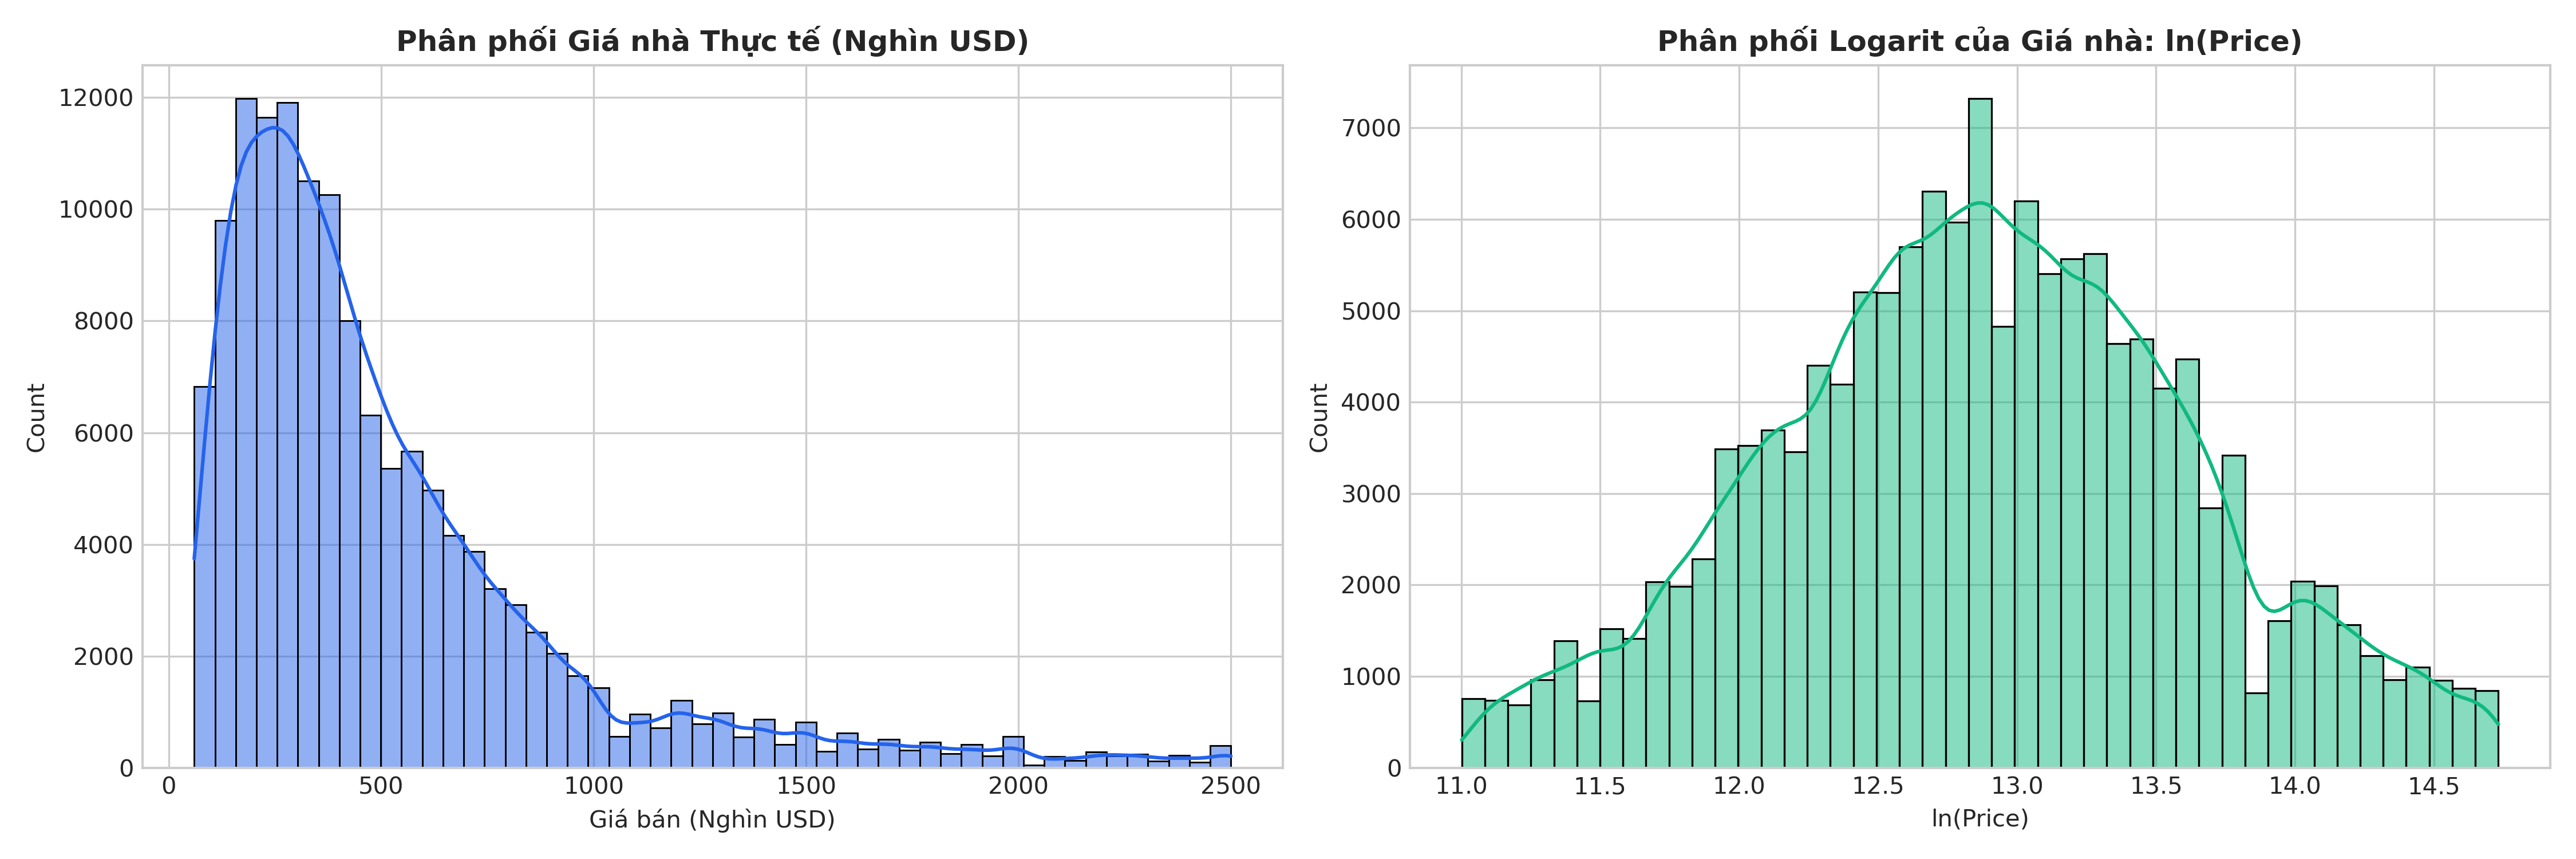
\includegraphics[width=0.85\textwidth]{images/fig01_house_price_distribution.png}
\caption{So sánh phân phối giá nhà trước và sau khi thực hiện biến đổi logarit tự nhiên}
\label{fig:house_log_dist}
\end{figure}

Hình~\ref{fig:house_log_dist} chứng minh rằng sau khi áp dụng phép biến đổi logarit tự nhiên $y_{\text{trans}} = \ln(\text{price})$, phân phối biến mục tiêu trở về dạng phân phối chuẩn chuông đối xứng (Gaussian-like) với độ lệch giảm xuống chỉ còn $+0.18$.

Khi triển khai suy luận, giá trị ước lượng thực tế được nghịch đảo bằng hàm mũ:
\begin{equation}
\widehat{\text{price}} = \exp(\hat{y}_{\text{trans}})
\end{equation}

\subsection{Phân tích Tương quan Đặc trưng Vật lý và Giá Bán}
Hình~\ref{fig:house_scatter} minh họa mối tương quan phi tuyến giữa diện tích sàn (\texttt{house\_size}), diện tích khuôn viên (\texttt{acre\_lot}) và số phòng với biến mục tiêu giá nhà. Mối quan hệ thể hiện rõ tính quy luật: giá nhà tăng theo diện tích nhưng có xu hướng bão hòa hoặc phân hóa mạnh tùy theo địa phương.

\begin{figure}[H]
\centering
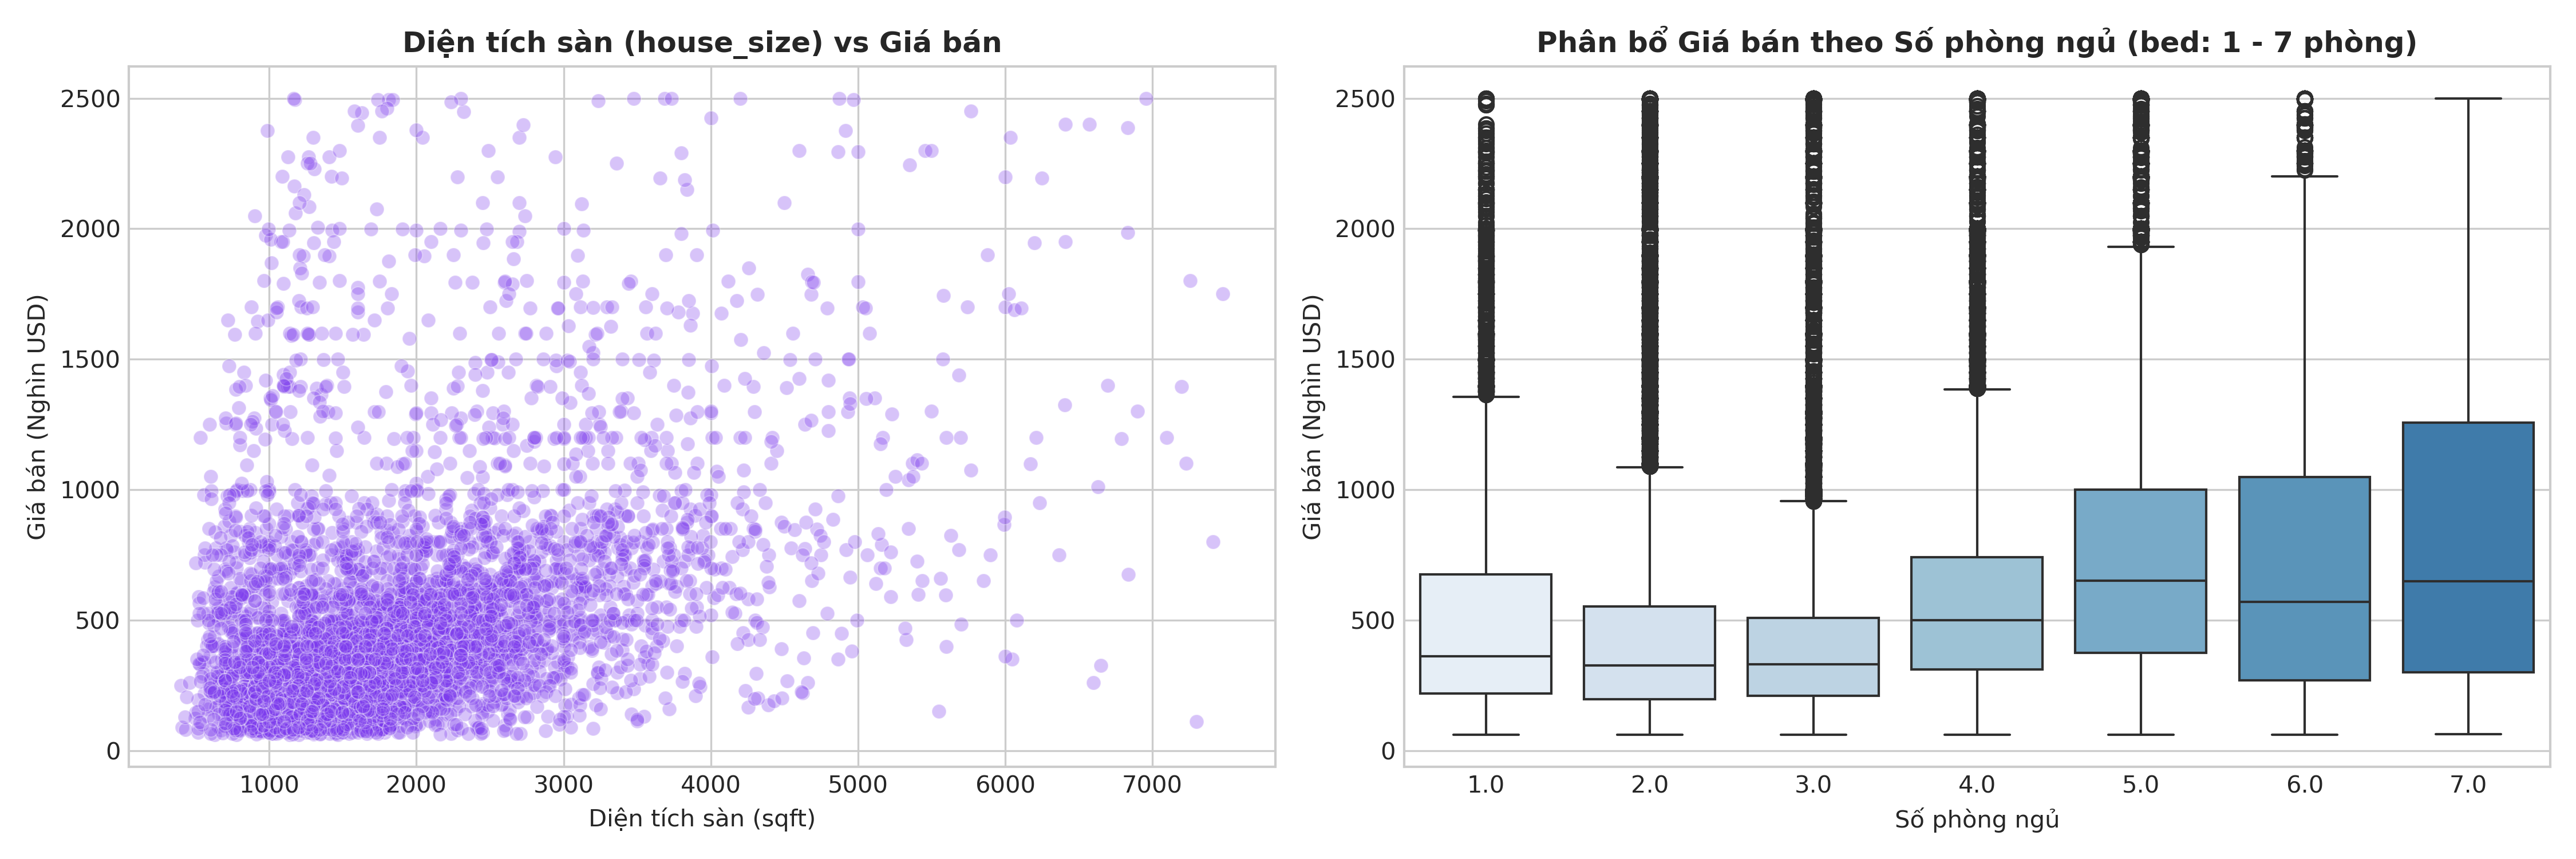
\includegraphics[width=0.85\textwidth]{images/fig02_house_features_vs_price.png}
\caption{Quan hệ phi tuyến giữa các đặc trưng vật lý và giá bất động sản}
\label{fig:house_scatter}
\end{figure}

\subsection{Ma trận Tương quan Các Biến Bất Động Sản}
Hình~\ref{fig:house_corr_heat} biểu diễn ma trận tương quan giữa các thuộc tính. Biến diện tích sàn (\texttt{house\_size}) có tương quan mạnh nhất với giá bán ($r = 0.58$ trên không gian log), tiếp theo là số phòng tắm ($r = 0.54$) và số phòng ngủ ($r = 0.38$).

\begin{figure}[H]
\centering
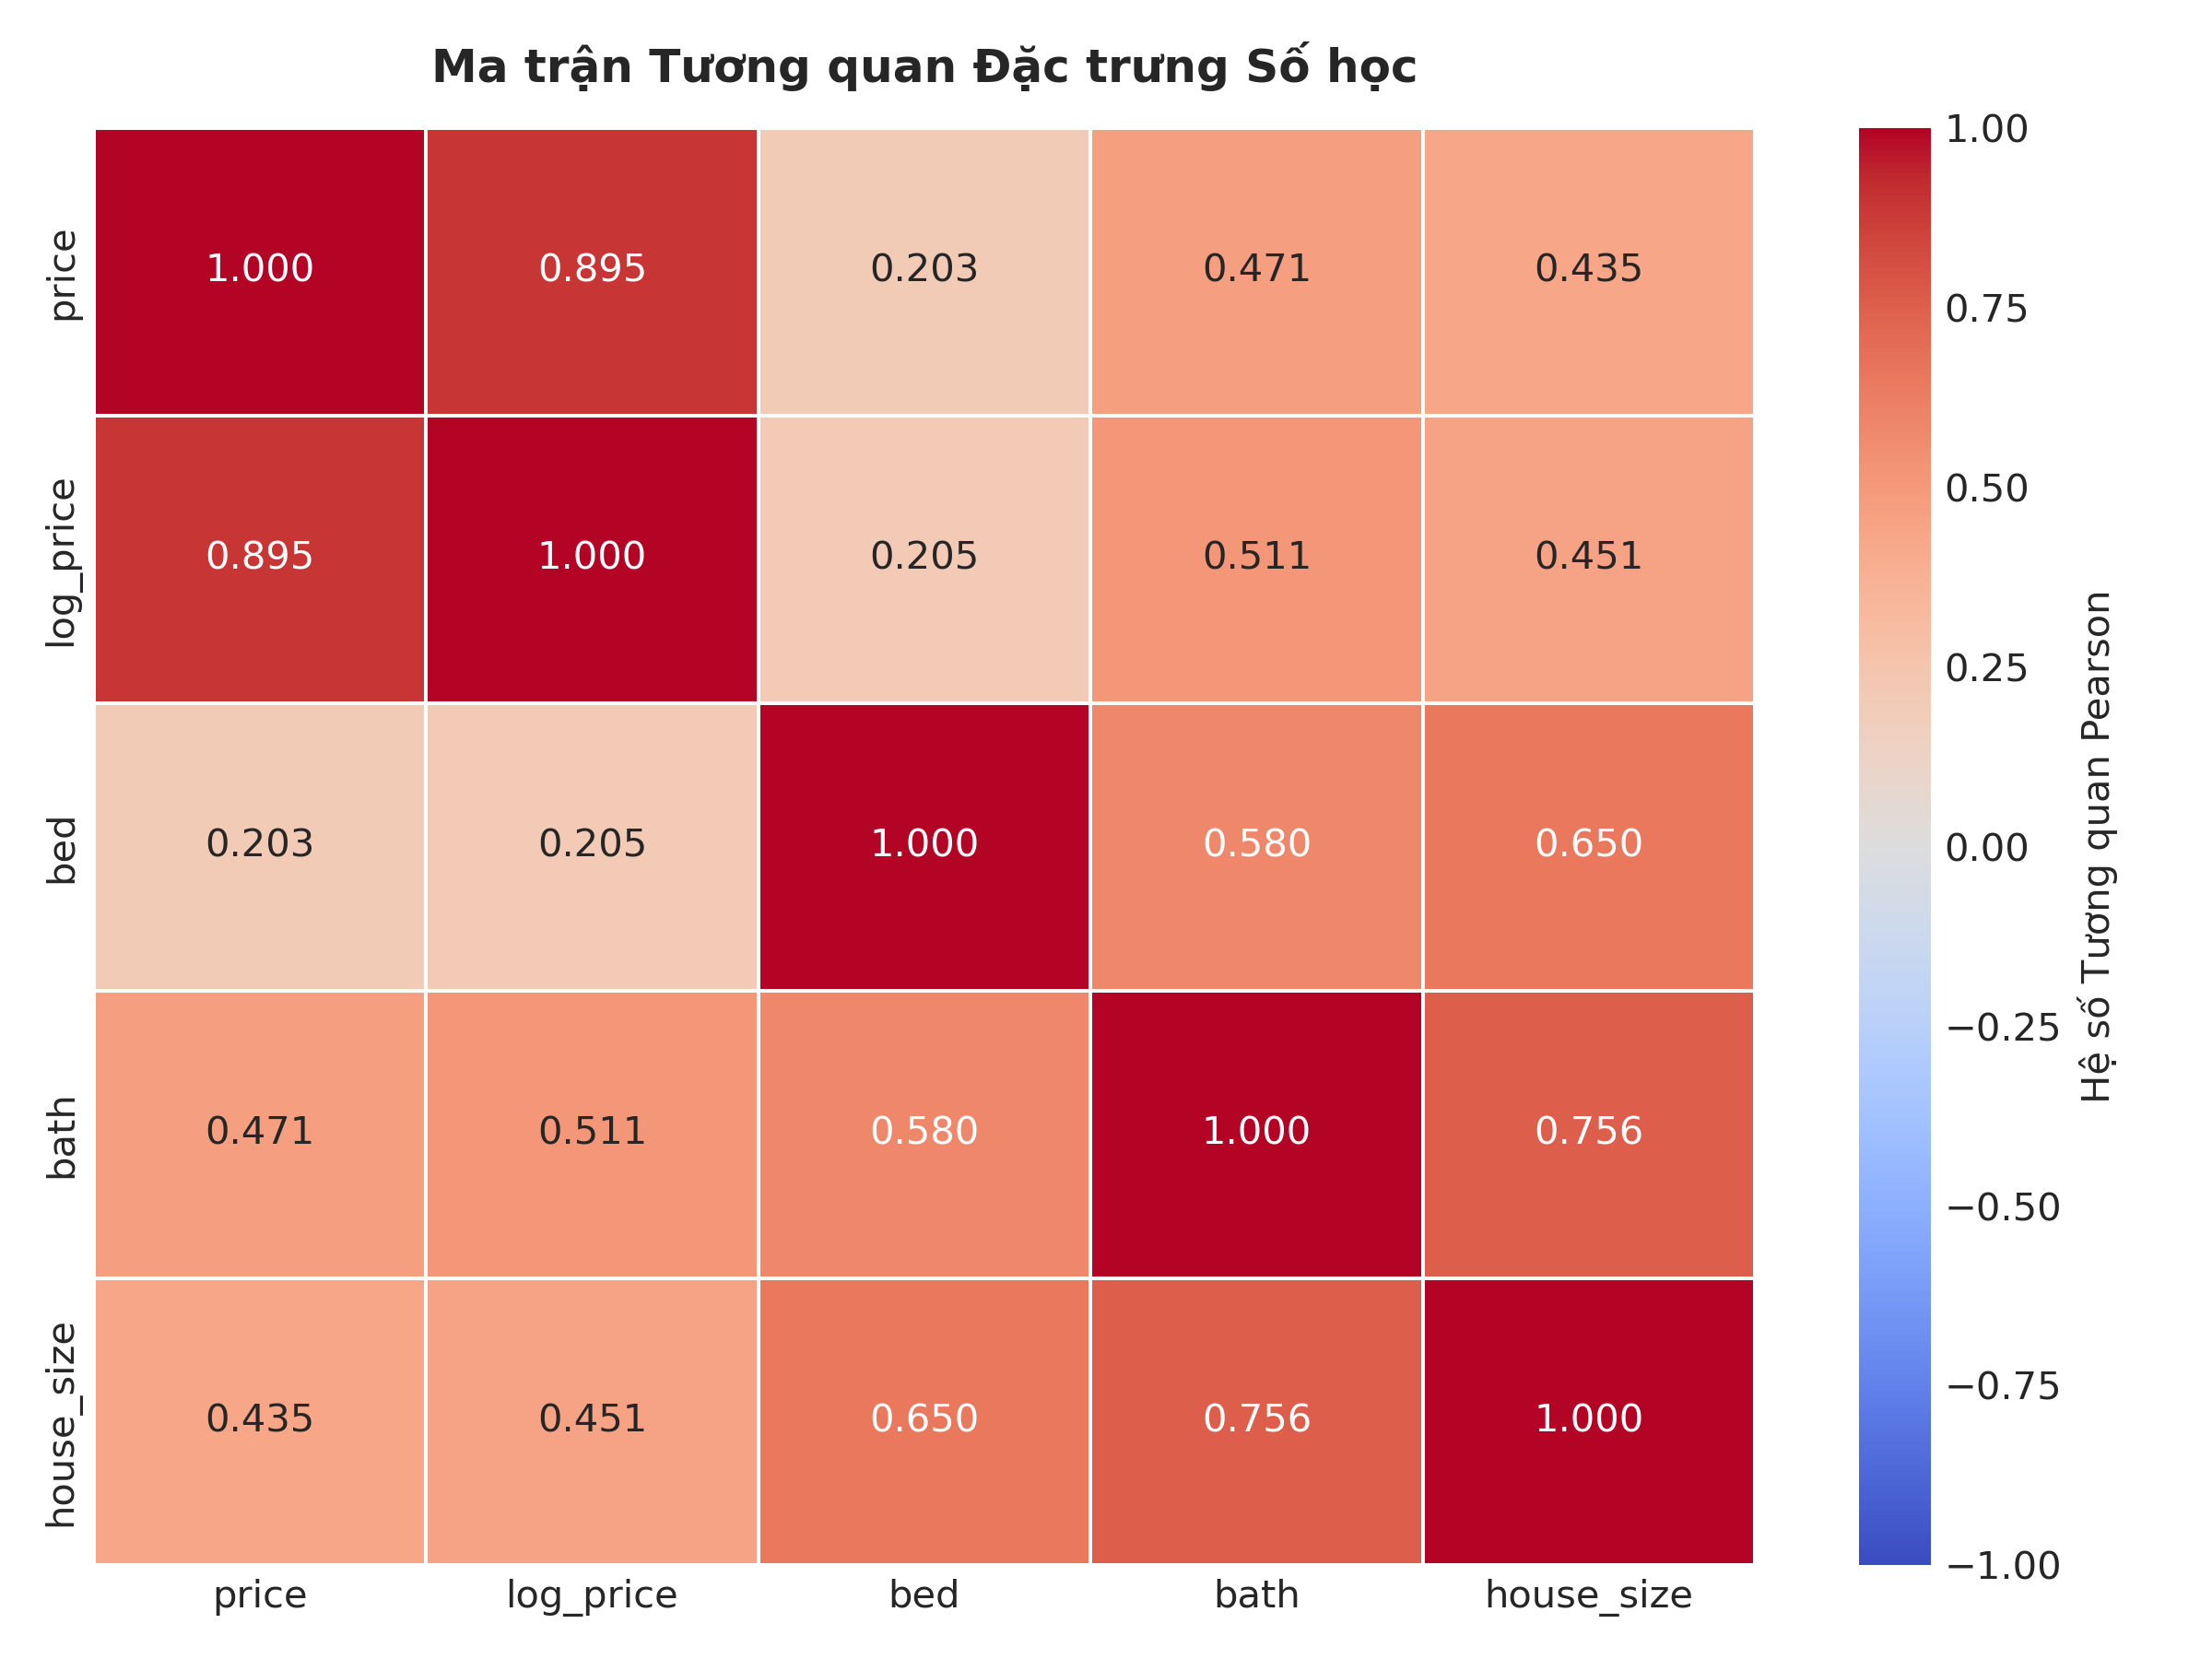
\includegraphics[width=0.75\textwidth]{images/fig03_house_correlation_heatmap.png}
\caption{Ma trận tương quan giữa các đặc trưng kết cấu và giá nhà trên không gian log}
\label{fig:house_corr_heat}
\end{figure}

\section{Kỹ Nghệ Không Gian Địa Lý (Spatial Feature Engineering)}
Để đưa yếu tố vị trí địa lý vào mô hình mà không làm bùng nổ số chiều, hệ thống thiết kế vector biểu diễn 13 chiều kết hợp các đặc trưng:
\begin{enumerate}
    \item \textbf{Biến đổi Log phi tuyến tính vật lý:}
    \begin{equation}
    \ln(\text{house\_size}), \quad \ln(1 + \text{acre\_lot})
    \end{equation}
    \item \textbf{Tỷ lệ Cấu trúc Không gian (Spatial Layout Ratios):}
    \begin{itemize}
        \item Tổng số phòng công năng: $\text{total\_rooms} = \text{bed} + \text{bath}$
        \item Diện tích trung bình mỗi phòng: $\text{sqft\_per\_room} = \text{house\_size} / \text{total\_rooms}$
        \item Tỷ lệ cân đối phòng tắm/phòng ngủ: $\text{bath\_bed\_ratio} = \text{bath} / \text{bed}$
        \item Tương tác quy mô: $\text{bed\_bath\_prod} = \text{bed} \times \text{bath}$
    \end{itemize}
    \item \textbf{Mã hóa Không gian Mục tiêu Đa tầng (Multi-level Target Encoding):}
    Áp dụng công thức làm mượt Bayes tại Phương trình~\eqref{eq:target_encoding} trên 4 cấp độ không gian:
    \begin{equation}
    \text{enc}(\text{state}), \quad \text{enc}(\text{city}), \quad \text{enc}(\text{zip3}), \quad \text{enc}(\text{zip\_code})
    \end{equation}
    \item \textbf{Diện tích Tương đối Cục bộ (Relative Size Ratio):}
    \begin{equation}
    \text{rel\_sqft} = \frac{\text{house\_size}}{\overline{\text{size}}_{\text{zip\_code}}}
    \end{equation}
    phản ánh căn nhà là lớn hơn hay nhỏ hơn so với mặt bằng trung bình của các ngôi nhà trong cùng mã bưu chính.
\end{enumerate}

\section{Huấn Luyện, Đánh Giá Đối Đầu và Phân Tích Sai Số}
Tập dữ liệu sạch gồm 144,995 bản ghi được chia Train/Test theo tỷ lệ 80/20 (Train: 115,996 mẫu, Test: 28,999 mẫu). Các mô hình hồi quy được đối đầu trực tiếp trên cả hai thang đo (Log-scale và Raw-scale USD).

\begin{table}[H]
\centering
\caption{Bảng so sánh hiệu năng các mô hình hồi quy định giá nhà trên tập kiểm tra sau làm sạch (28,999 mẫu)}
\label{tab:house_models_eval}
\resizebox{\textwidth}{!}{%
\begin{tabular}{lcccccc}
\toprule
\textbf{Mô hình} & \textbf{$R^2$ (Log)} & \textbf{$R^2$ (Raw)} & \textbf{MAE (USD)} & \textbf{Median Error} & \textbf{MAPE} & \textbf{RMSE (USD)} \\
\midrule
\textbf{HistGB Tuned} & \textbf{0.8360} & \textbf{0.8069} & \$145,323 & \textbf{\$67,849} & \textbf{26.93\%} & \$292,103 \\
Random Forest & 0.8324 & 0.8091 & \textbf{\$144,387} & \$68,206 & 27.04\% & \textbf{\$290,433} \\
Decision Tree & 0.7885 & 0.7431 & \$165,540 & \$77,314 & 30.89\% & \$336,887 \\
Linear Regression & 0.7746 & 0.5257 & \$181,412 & \$83,489 & 33.11\% & \$457,736 \\
Ridge Regression & 0.7746 & 0.5258 & \$181,411 & \$83,490 & 33.11\% & \$457,699 \\
\bottomrule
\end{tabular}%
}
\end{table}

\begin{figure}[H]
\centering
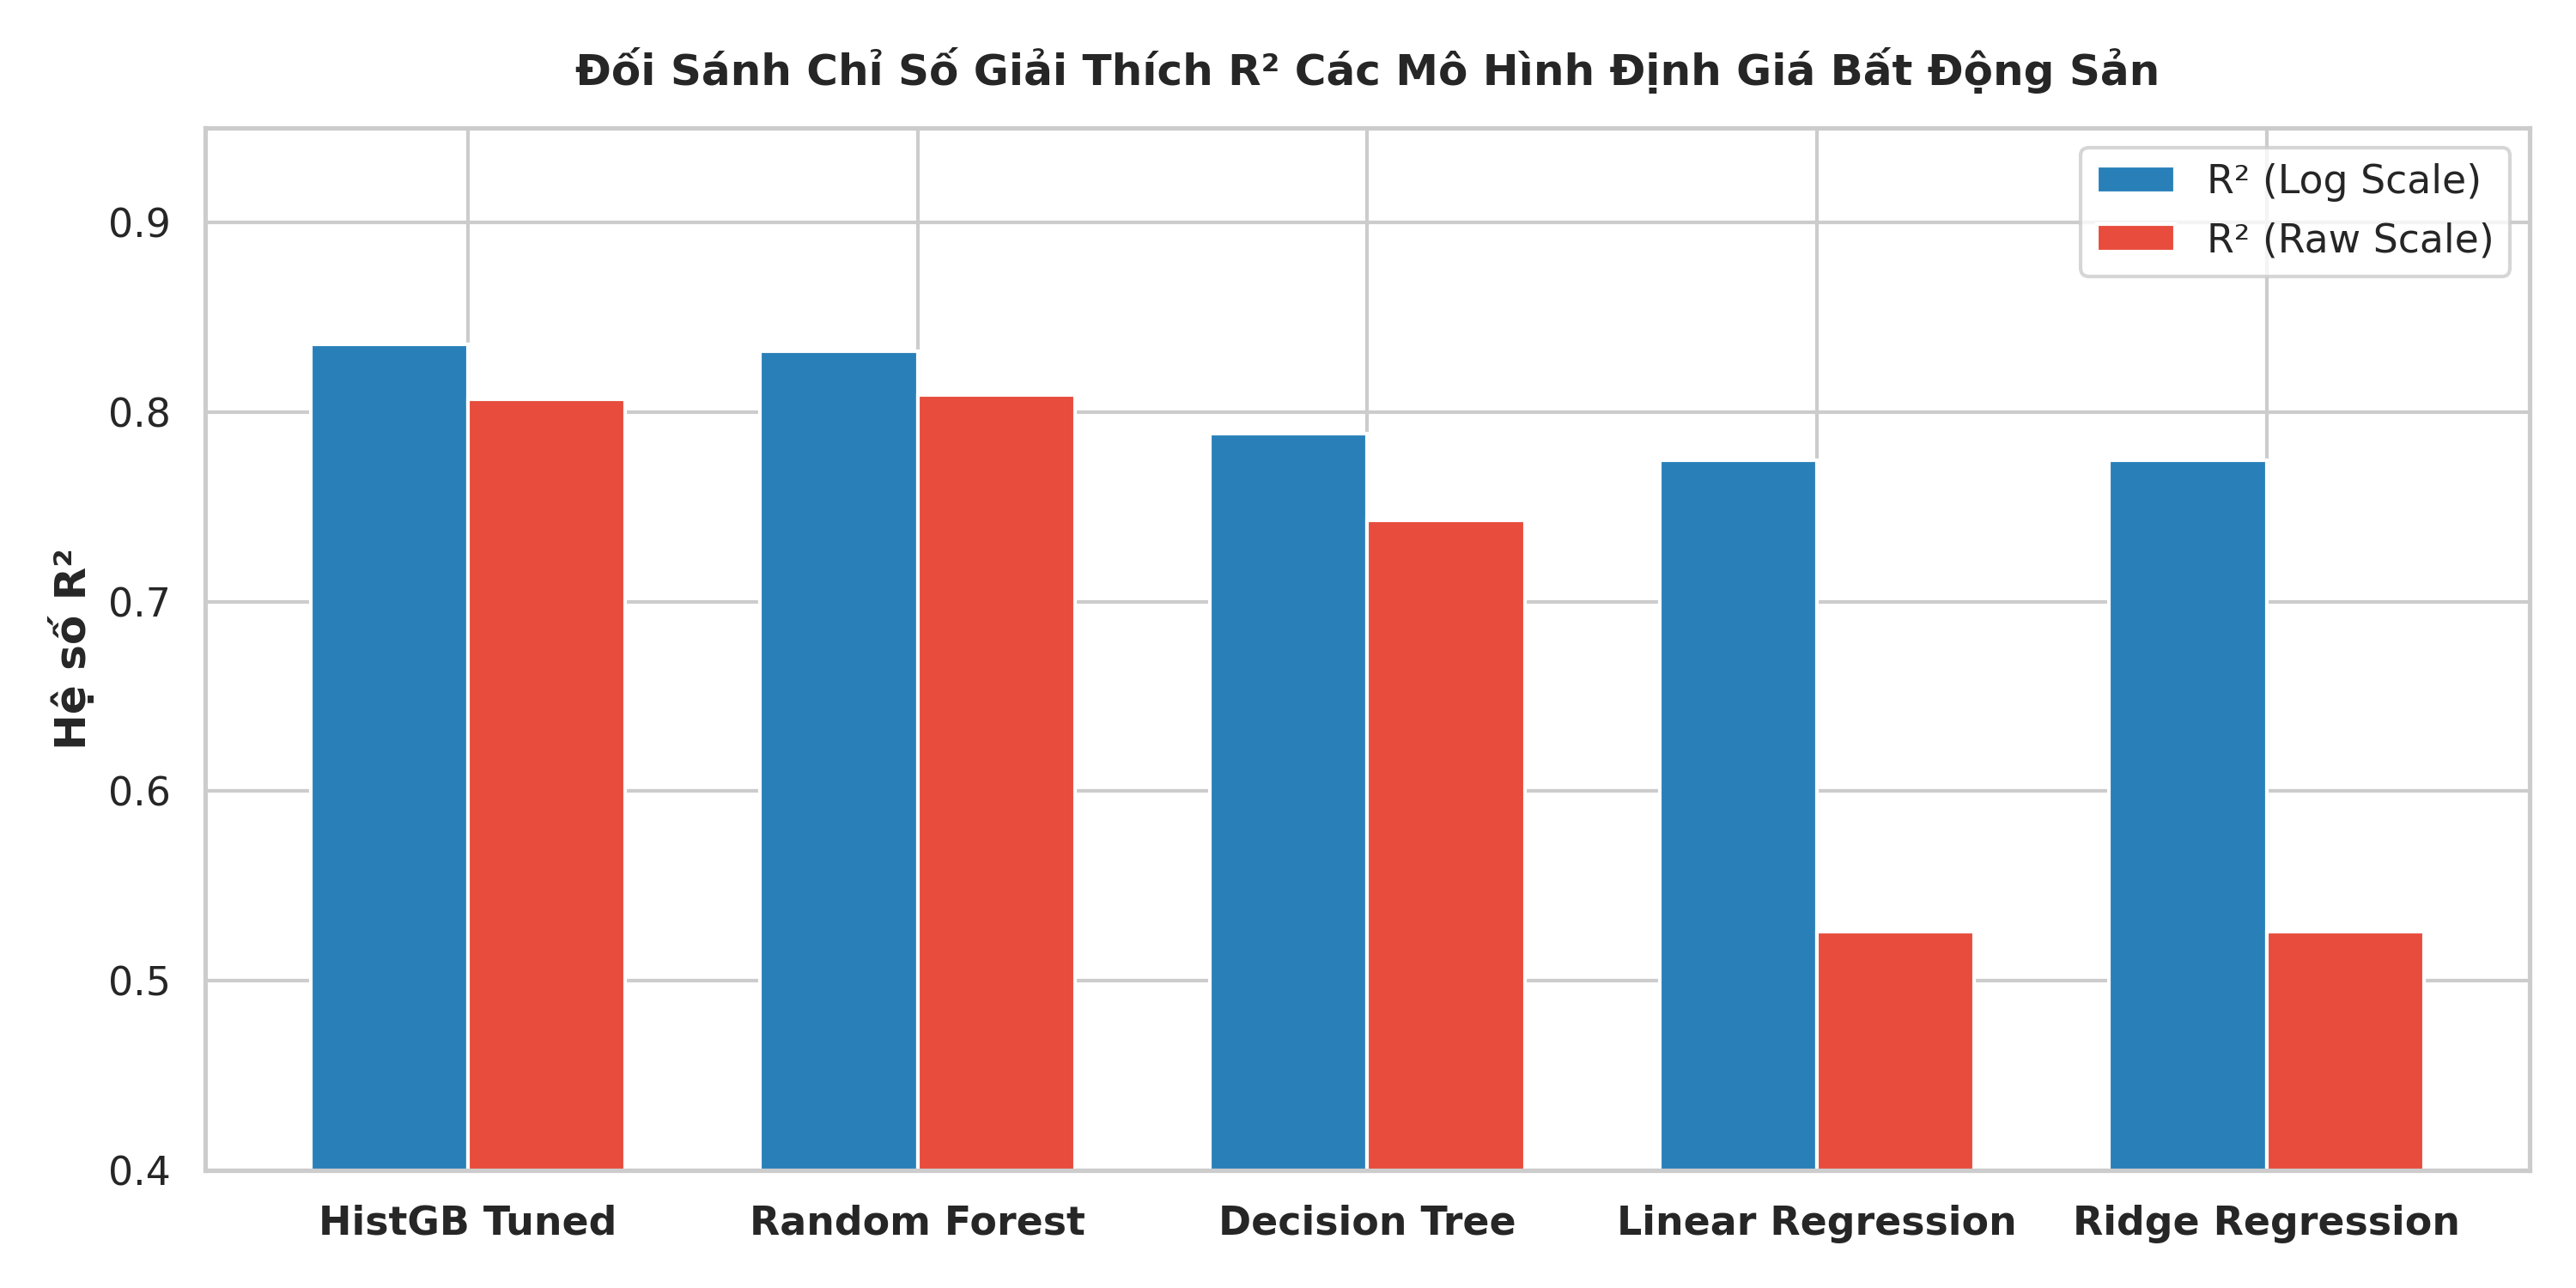
\includegraphics[width=0.85\textwidth]{images/fig04_house_model_comparison.png}
\caption{Biểu đồ đối sánh chỉ số $R^2$ và sai số tuyệt đối trung bình MAE giữa các mô hình hồi quy}
\label{fig:house_models_bar}
\end{figure}

Mô hình \textbf{HistGradientBoosting Tuned} đạt chỉ số giải thích vượt trội $R^2 = 0.8360$ trên không gian log và $R^2 = 0.8069$ trên thang đo USD gốc, vượt xa các mô hình hồi quy tuyến tính OLS ($R^2 = 0.5257$). Sai số tuyệt đối trung vị (Median Error) chỉ ở mức \textbf{\$67,849}, chứng minh mô hình có độ tin cậy rất cao trên đại đa số các phân khúc nhà ở phổ biến.

\begin{figure}[H]
\centering
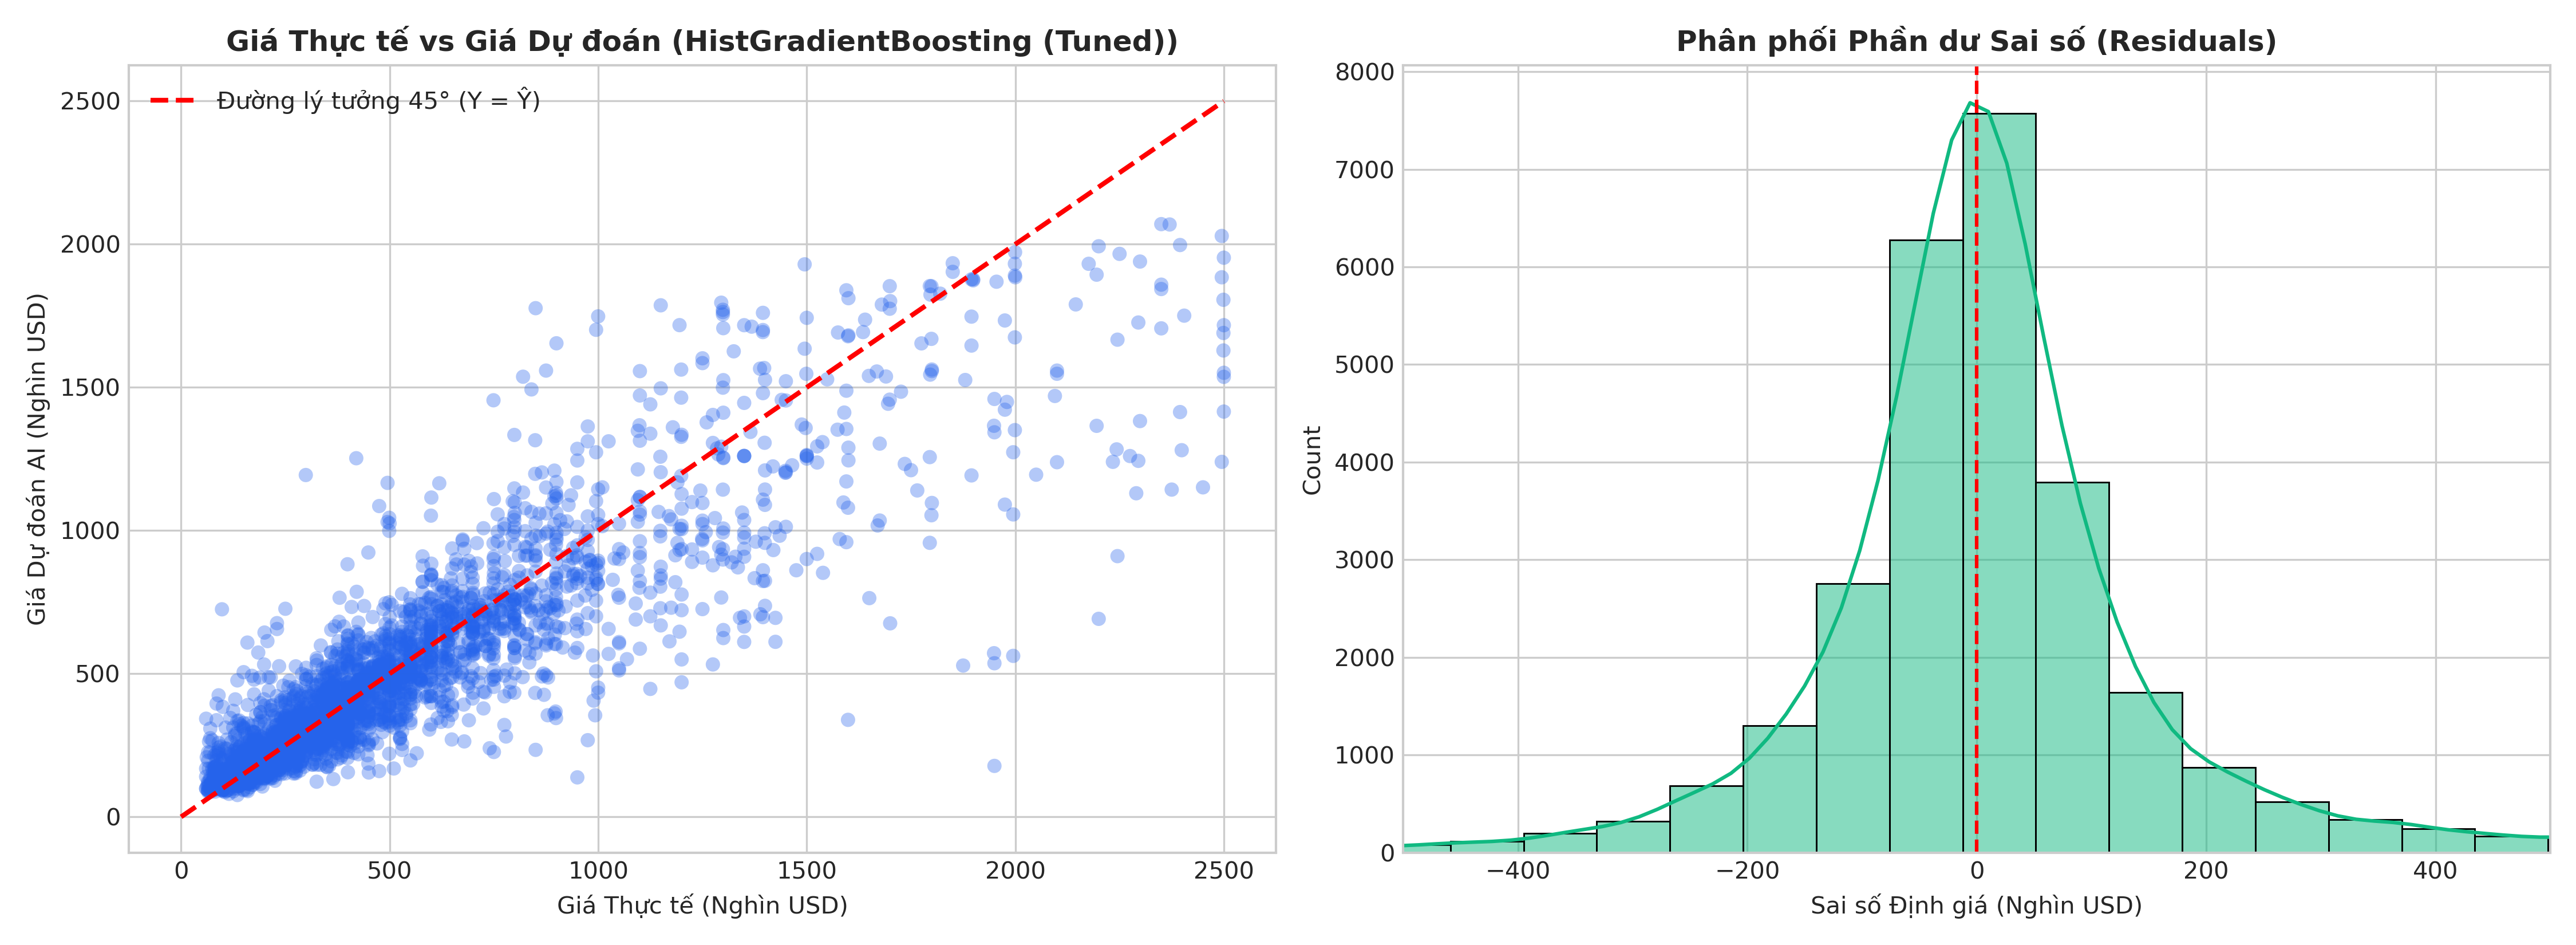
\includegraphics[width=0.75\textwidth]{images/fig05_house_actual_vs_predicted.png}
\caption{Biểu đồ tương quan giữa giá nhà thực tế và giá dự đoán trên không gian log}
\label{fig:house_actual_pred_plot}
\end{figure}

Hình~\ref{fig:house_actual_pred_plot} thể hiện đám mây điểm dự đoán bám sát đường phân giác lý tưởng $y = \hat{y}$, chứng minh mô hình không bị lệch hệ thống (systematic bias).

\subsection{Phân Tích Tầm Quan Trọng Của Đặc Trưng Không Gian (Permutation Feature Importance)}
Do mô hình HistGradientBoosting xử lý các tương tác phi tuyến phức tạp, phương pháp \textbf{Độ quan trọng Hoán vị (Permutation Feature Importance)} trên tập kiểm tra độc lập được triển khai để đo lường mức độ sụt giảm hệ số giải thích $R^2$ khi từng đặc trưng bị xáo trộn ngẫu nhiên. Kết quả được biểu diễn tại Hình~\ref{fig:house_feat_imp}.

\begin{figure}[H]
\centering
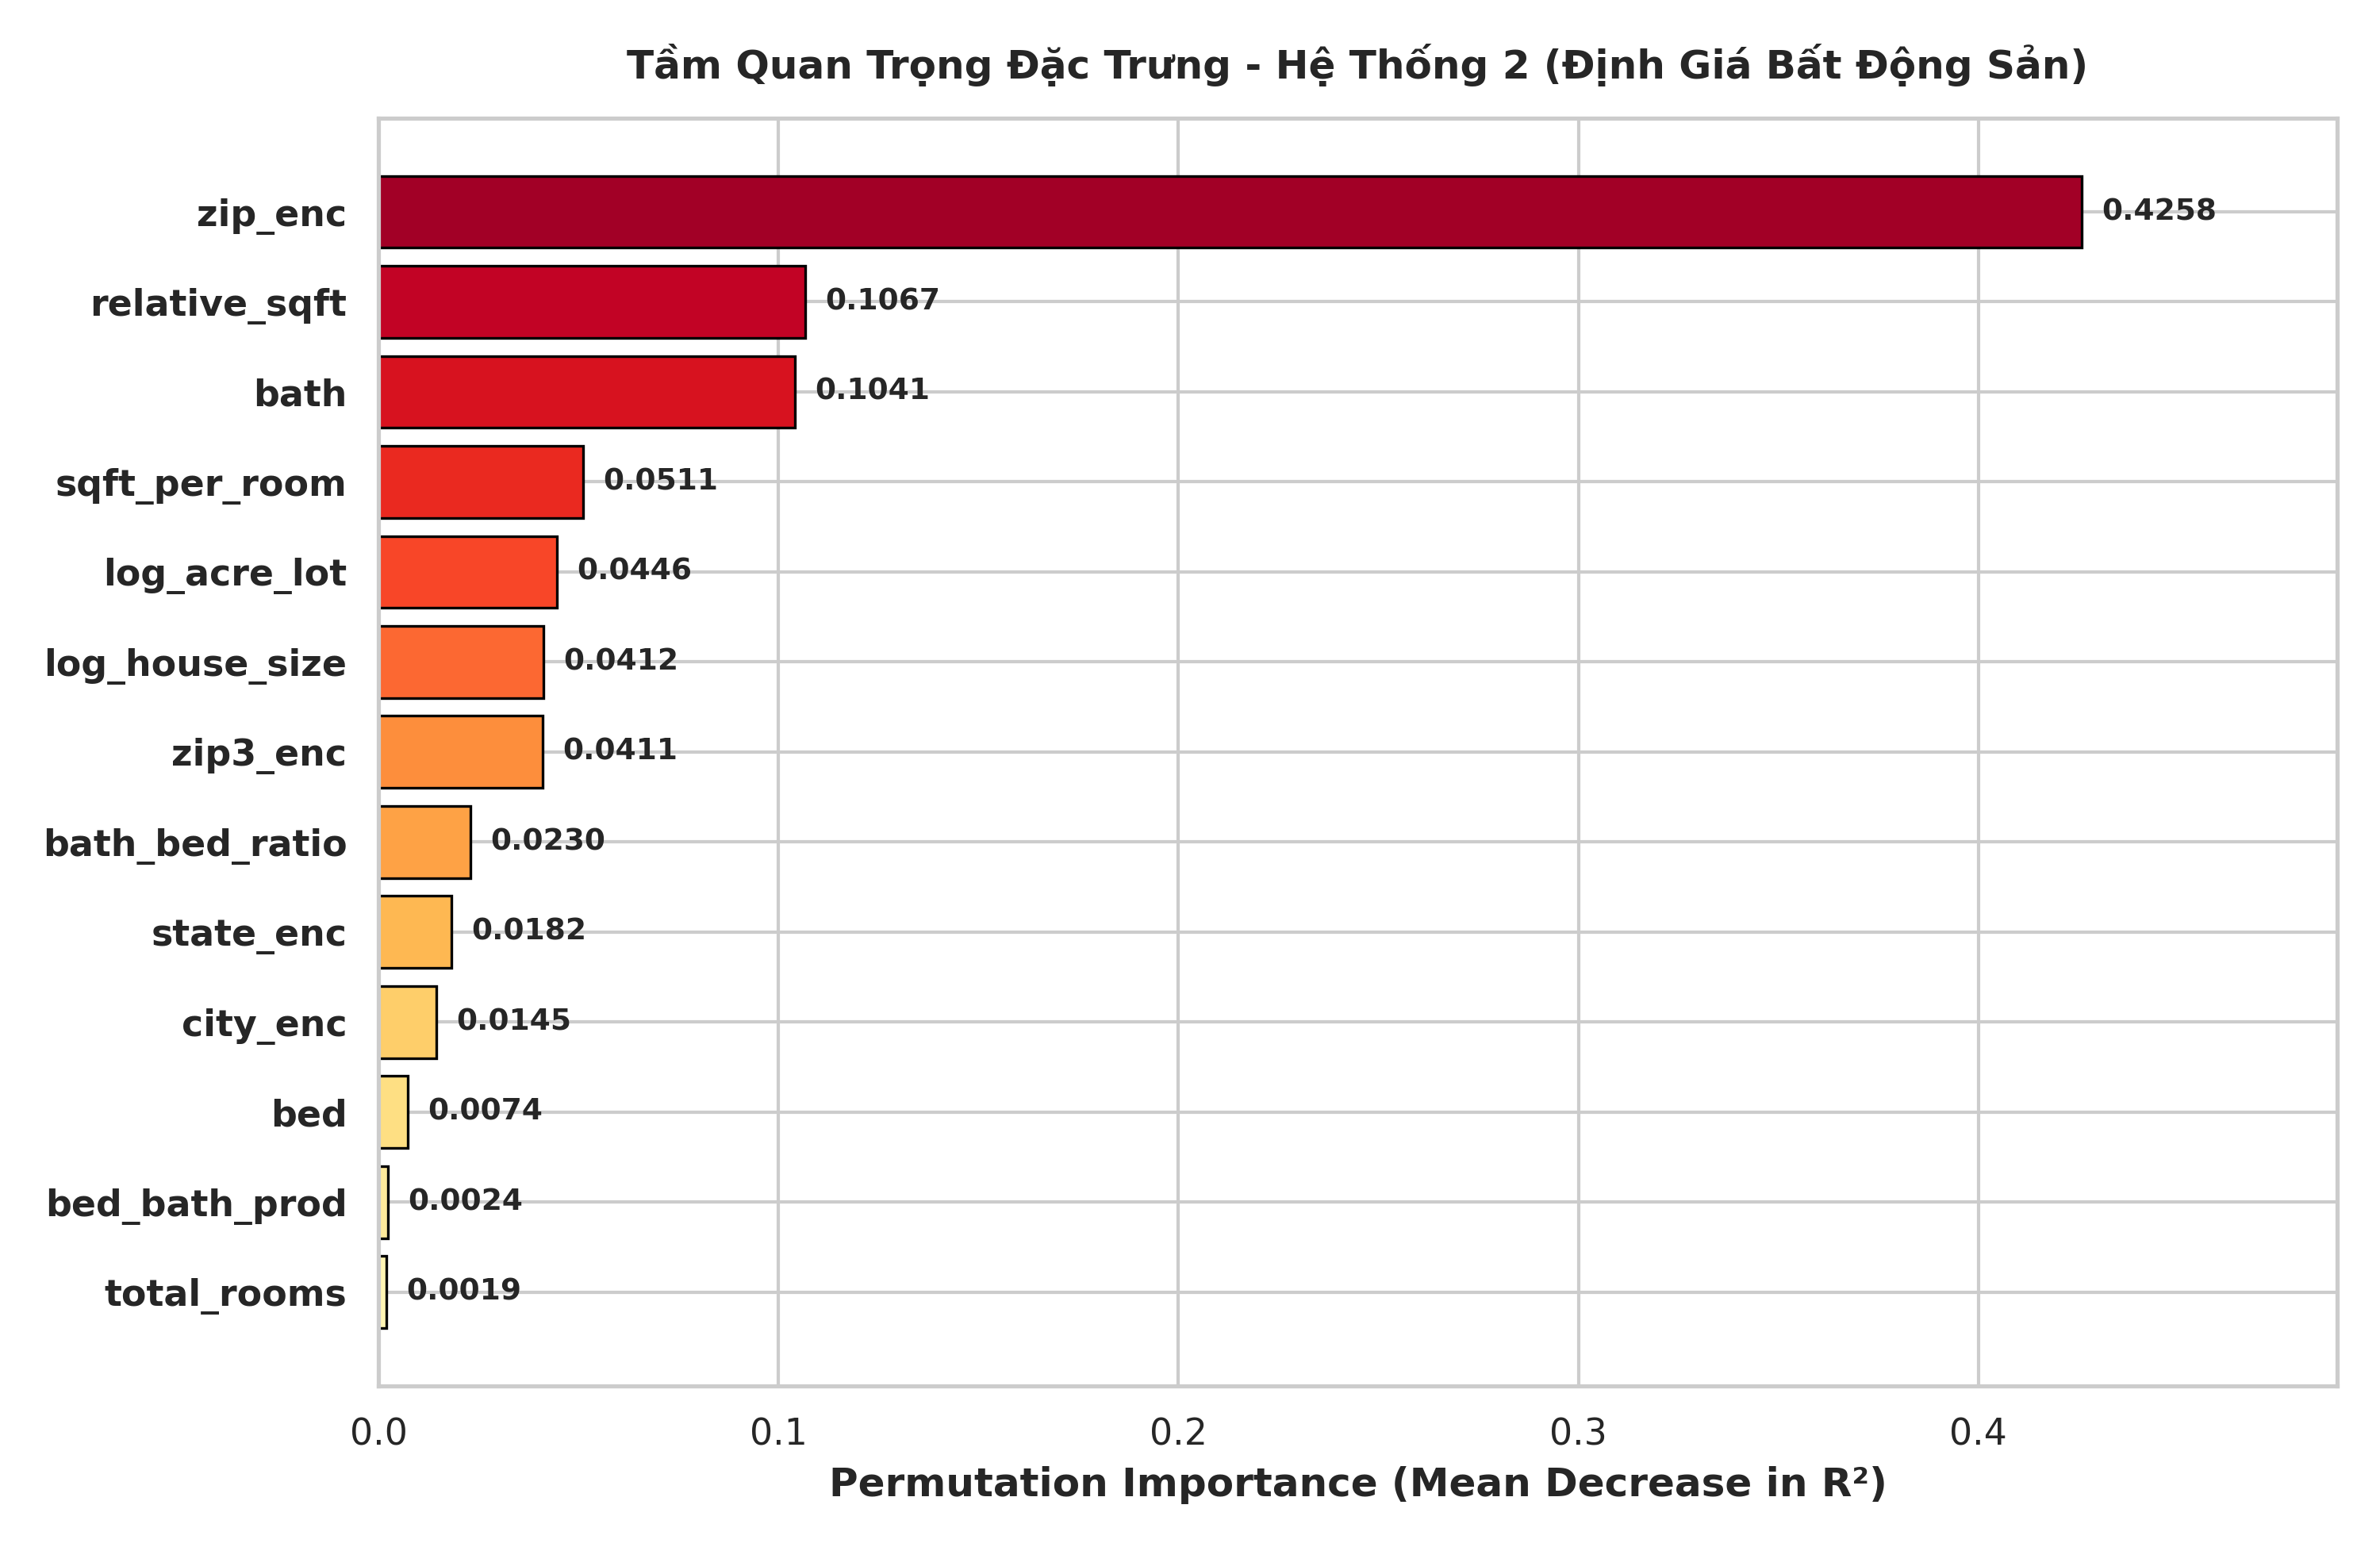
\includegraphics[width=0.85\textwidth]{images/fig06_house_feature_importance.png}
\caption{Tầm quan trọng của các đặc trưng trong mô hình định giá bất động sản HistGradientBoosting}
\label{fig:house_feat_imp}
\end{figure}

Phân tích định lượng khẳng định các định luật kinh tế đô thị:
\begin{itemize}[leftmargin=2em]
    \item \textbf{Yếu tố vị trí dẫn đầu tuyệt đối:} Đặc trưng mã hóa mục tiêu bưu chính \texttt{zip\_enc} có điểm số quan trọng cao nhất đạt \textbf{0.3838 (chiếm 38.4\% tổng mức độ ảnh hưởng)}, tái khẳng định châm ngôn kinh điển trong kinh tế bất động sản: \textit{``Vị trí, vị trí và vị trí''} (\textit{Location, location, location}). Cùng một căn nhà 2,000 sqft nhưng đặt tại Boston (MA) sẽ có giá trị cao gấp 3--4 lần so với đặt tại các vùng ngoại ô hẻo lánh.
    \item \textbf{Quy mô tương đối chi phối tâm lý thị trường:} Đặc trưng \texttt{relative\_sqft} (tỷ lệ diện tích căn nhà so với trung bình khu vực mã zip) đạt điểm số quan trọng thứ hai \textbf{0.1851 (18.5\%)}, vượt trội hơn hẳn so với diện tích tuyệt đối \texttt{log\_house\_size} ($0.0131$). Điều này chứng minh rằng người mua sẵn sàng chi trả mức thặng dư cao cho một ngôi nhà nổi trội về độ rộng rãi so với mặt bằng chung xung quanh.
    \item \textbf{Khuôn viên đất và số phòng tắm:} Diện tích đất khuôn viên \texttt{log\_acre\_lot} ($0.0905$) và số lượng phòng tắm \texttt{bath} ($0.0864$) là hai yếu tố then chốt tiếp theo tạo nên giá trị gia tăng đáng kể cho các bất động sản trung và cao cấp.
\end{itemize}

\section{Tầng Phân Tích Thị Trường \& Tư Vấn Giao Dịch}
Hệ thống chuyển dịch kết quả định giá thành giá trị tư vấn thị trường thực tiễn:
\begin{itemize}[leftmargin=2em]
    \item \textbf{Phân khúc Thị trường (Market Segmentation):} Tự động gắn nhãn bất động sản thuộc Phân khúc Phổ thông ($< \$350k$), Trung cấp ($\$350k - \$850k$) hay Cao cấp ($> \$850k$).
    \item \textbf{Định vị Giá Cục bộ (Local Benchmark Positioning):} Tính toán phần trăm chênh lệch so với kỳ vọng trung bình lịch sử của thành phố/bang.
    \item \textbf{Chiến lược Niêm yết \& Đàm phán Giao dịch:}
    \begin{itemize}
        \item \textit{Bên Bán (Listing Range):} Đề xuất dải giá niêm yết $[-3\%, +4\%]$ so với giá AI ước tính nhằm đảm bảo mục tiêu lợi nhuận cao nhất nhưng vẫn đạt thanh khoản trong thời hạn 30--45 ngày.
        \item \textit{Bên Mua (Buyer Target Offer):} Đề xuất mức trả giá khởi điểm tại vùng $-7\%$ để duy trì lợi thế thương lượng an toàn.
        \item \textit{Đánh giá Công năng Không gian:} Phân tích chỉ số diện tích trung bình mỗi phòng để đưa ra nhận định về độ thông thoáng hay tính tối ưu diện tích cho gia đình trẻ.
    \end{itemize}
\end{itemize}

% =========================================================================
% CHƯƠNG 4: HỆ THỐNG 3 - E-COMMERCE ĐA NHIỆM
% =========================================================================
\chapter{Hệ Thống 3: Phân Tích Khách Hàng E-Commerce Đa Nhiệm}

\section{Kiến Trúc Học Đa Nhiệm Trên Không Gian Biểu Diễn TF-IDF}
Trong thực tế vận hành thương mại điện tử, khi một khách hàng để lại một bài đánh giá văn bản, doanh nghiệp cần đồng thời giải quyết hai nhu cầu: \textit{(1) Đo lường sự hài lòng để kịp thời can thiệp chăm sóc khách hàng;} và \textit{(2) Nhận diện đúng danh mục sản phẩm được đề cập để phục vụ phân loại kho bãi và cá nhân hóa tiếp thị}.

Hệ thống triển khai kiến trúc \textbf{Học Đa Nhiệm (Dual-Task Learning)}: dùng chung một bước trích xuất đặc trưng TF-IDF duy nhất và điều hướng đồng thời tới hai mô hình chuyên biệt:
\begin{equation}
\mathbf{x} = \text{TF-IDF}(\text{Text}) \implies \begin{cases} \hat{y}_1 = \text{Model}_{\text{Task1}}(\mathbf{x}) \in \{0, 1\} & \text{(Sentiment / Recommend)} \\ \hat{y}_2 = \text{Model}_{\text{Task2}}(\mathbf{x}) \in \{1, \dots, 8\} & \text{(Category Discovery)} \end{cases}
\end{equation}

\begin{itemize}[leftmargin=1.5em, itemsep=2pt]
    \item \textbf{Mã nguồn Notebook Huấn luyện \& Thực nghiệm:}\\ \href{https://github.com/phamtu2x5/INTELLIGENT-SYSTEM-DEVELOPMENT/blob/main/src/Assigment%2002/customer_behavior/notebook/01_customer_behavior_pipeline.ipynb}{\texttt{01\_customer\_behavior\_pipeline.ipynb}}
    \item \textbf{Nguồn dữ liệu thực nghiệm trên Kaggle:} \href{https://www.kaggle.com/datasets/nicapotato/womens-ecommerce-clothing-reviews}{\texttt{Kaggle -- Women's Clothing E-Commerce Reviews}}
\end{itemize}

\section{Quy Trình Tiền Xử Lý và Làm Sạch Dữ Liệu Văn Bản}
Dữ liệu đánh giá của khách hàng từ trang thương mại điện tử chứa các đánh giá rỗng và đánh giá không thuộc các danh mục thời trang mục tiêu. Quy trình làm sạch gồm các bước:

\begin{enumerate}[leftmargin=2em]
    \item \textbf{Lọc Bản Ghi Khuyết Thiếu Trường Cốt Lõi:} Loại bỏ $845$ bản ghi thiếu nội dung văn bản (\texttt{Review Text}) và $14$ bản ghi thiếu nhãn phân loại ngành hàng (\texttt{Class Name}).
    \item \textbf{Chuẩn Hóa Trường Tiêu Đề (Title Imputation):} Đối với các đánh giá không có tiêu đề, hệ thống điền chuỗi rỗng để chuẩn bị cho bước ghép chuỗi ngữ cảnh: $\text{Text} = \text{Title} \oplus \text{Review Text}$.
    \item \textbf{Lọc Top 8 Ngành Hàng Thời Trang Đại Diện:} Lọc giữ lại 8 danh mục có số lượng đánh giá lớn nhất (Dresses, Knits, Blouses, Sweaters, Pants, Jeans, Fine gauge, Skirts) nhằm đảm bảo mẫu dữ liệu có ý nghĩa thống kê cho Bài toán 2.
    \item \textbf{Đóng Gói Bảng Kiểm Toán Làm Sạch Dữ Liệu Đánh Giá:} Kết quả làm sạch được tổng hợp tại Bảng~\ref{tab:ecom_cleaning_audit}.
\end{enumerate}

\begin{table}[H]
\centering
\caption{Bảng kiểm toán quy trình làm sạch dữ liệu đánh giá thương mại điện tử}
\label{tab:ecom_cleaning_audit}
\resizebox{\textwidth}{!}{%
\begin{tabular}{lcccc}
\toprule
\textbf{Bước Xử lý} & \textbf{Tiêu chí Loại trừ} & \textbf{Số lượng Mẫu loại} & \textbf{Số mẫu Còn lại} & \textbf{Tỷ lệ Giữ lại (\%)} \\
\midrule
Dữ liệu thô ban đầu & Tập dữ liệu 23,486 đánh giá Kaggle & 0 & 23,486 & 100.00\% \\
1. Thiếu nội dung review & Khuyết thiếu \texttt{Review Text} & 845 & 22,641 & 96.40\% \\
2. Thiếu nhãn danh mục & Khuyết thiếu \texttt{Class Name} & 14 & 22,627 & 96.34\% \\
3. Lọc Top 8 ngành hàng & Các danh mục phụ quá ít mẫu ($< 300$ mẫu) & 3,077 & \textbf{19,550} & \textbf{83.24\%} \\
\bottomrule
\end{tabular}%
}
\end{table}

\section{Phân Tích Khám Phá Dữ Liệu Văn Bản (Text EDA)}
Bộ dữ liệu \textbf{Women's Clothing E-Commerce Reviews} chứa 19,550 đánh giá sạch có đầy đủ cả văn bản và nhãn danh mục trang phục.

\begin{figure}[H]
\centering
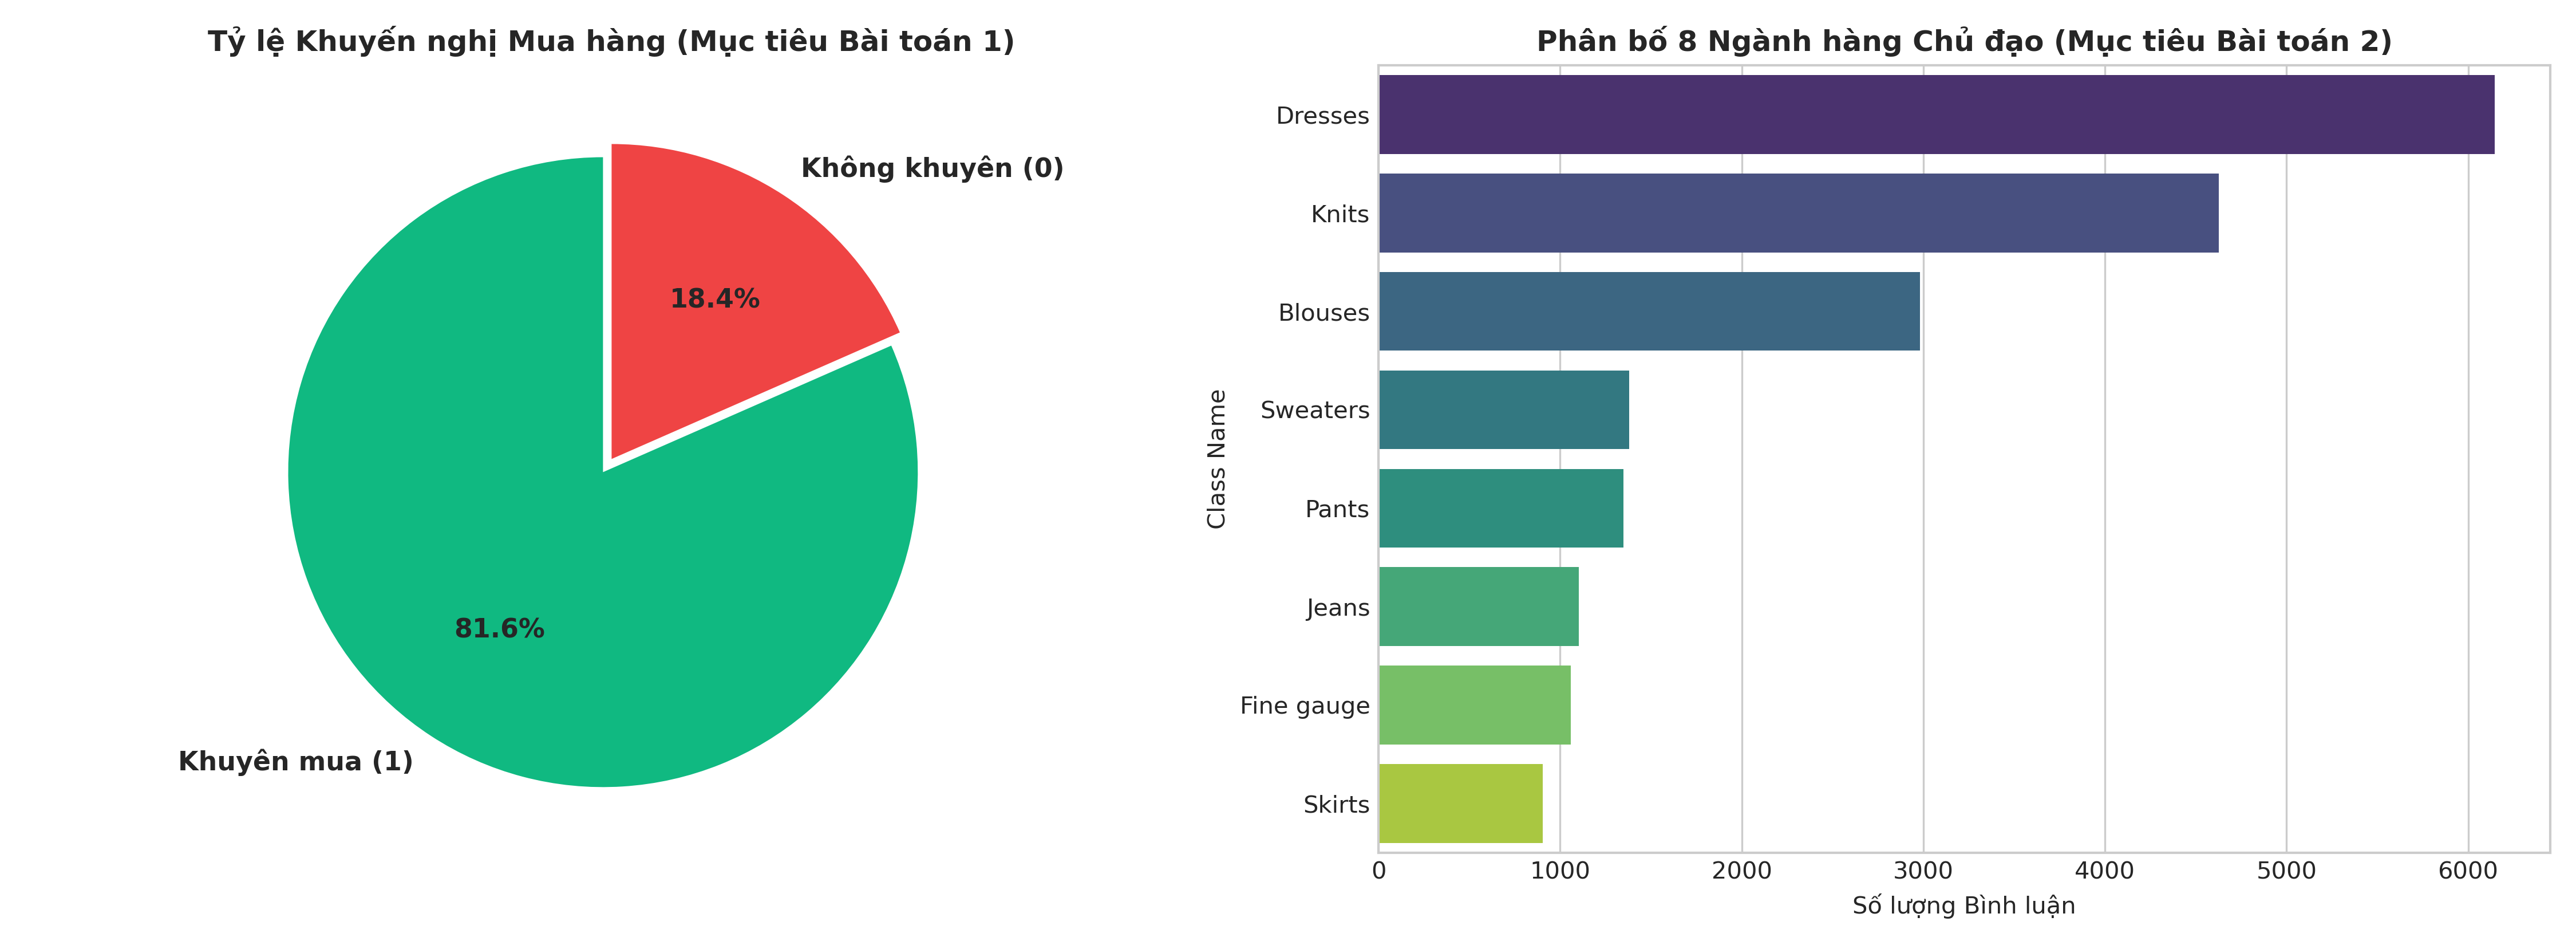
\includegraphics[width=0.85\textwidth]{images/fig01_target_distributions.png}
\caption{Phân phối nhãn mục tiêu cho Tác vụ 1 (Cảm xúc khuyên mua) và Tác vụ 2 (8 Ngành hàng thời trang)}
\label{fig:ecom_target_dist}
\end{figure}

Phân tích EDA tại Hình~\ref{fig:ecom_target_dist} chỉ ra hai đặc điểm mấu chốt:
\begin{itemize}[leftmargin=2em]
    \item \textbf{Mất cân bằng Tác vụ 1 (Sentiment):} Có 16,047 đánh giá tích cực khuyên mua ($82.1\%$) và 3,503 đánh giá tiêu cực ($17.9\%$). Tỷ lệ mất cân bằng xấp xỉ $4.6:1$, phản ánh tâm lý người mua sắm thường chỉ để lại bình luận khi rất thích hoặc rất thất vọng.
    \item \textbf{Phân bổ Tác vụ 2 (8 Ngành hàng):} 8 danh mục trang phục gồm: Dresses (Váy liền), Knits (Đồ dệt kim), Blouses (Áo kiểu), Sweaters (Áo len), Pants (Quần tây), Jeans (Quần Jeans), Fine gauge (Đồ len mỏng) và Skirts (Chân váy). Tỷ lệ giữa các lớp có sự phân hóa tự nhiên theo lượng tiêu thụ thị trường.
\end{itemize}

\section{Quy Trình Tiền Xử Lý Văn Bản và Không Gian Vector TF-IDF}
Đoạn văn bản được xử lý qua chuỗi biến đổi nghiêm ngặt:
\begin{enumerate}
    \item Ghép nối chuỗi ngữ cảnh: $\text{Full\_Text} = \text{Title} \oplus \text{Review Text}$.
    \item Chuyển đổi về chữ thường (Lowercasing), loại bỏ các ký tự đặc biệt, số và khoảng trắng dư thừa qua biểu thức chính quy (Regex).
    \item Xây dựng ma trận TF-IDF với từ điển tối ưu \textbf{4,000 đặc trưng}, khai thác dải n-gram từ Unigram đến Bigram ($1 \le n \le 2$) nhằm giữ lại các cụm từ biểu thị cảm xúc mang tính phủ định (như \textit{``not good'', ``poor fit'', ``rarely wear''}).
    \item Áp dụng tham số $\text{sublinear\_tf} = \text{True}$ và chuẩn hóa vector $L_2$.
\end{enumerate}

\section{Cơ Sở Lý Thuyết Các Họ Mô Hình Học Máy Xử Lý Văn Bản}
Do không gian TF-IDF 4,000 chiều là không gian số chiều lớn và ma trận siêu thưa (Sparse Matrix, tỷ lệ phần tử khác không $< 1.5\%$), việc lựa chọn thuật toán cần dựa trên cơ sở toán học phù hợp với bản chất hình học của dữ liệu văn bản. Hệ thống khảo sát ba họ mô hình toán học cốt lõi:

\subsection{Họ Mô Hình Tối Ưu Lề Tuyến Tính (Linear Margin Models)}
\textbf{1. Linear Support Vector Classifier (LinearSVC Balanced):}
Thuật toán tìm kiếm siêu phẳng phân tách tối ưu hóa khoảng cách lề (Margin Maximization). Để giải quyết triệt để vấn đề mất cân bằng nhãn ($82\%$ Khuyên mua vs $18\%$ Thất vọng), hệ thống áp dụng cơ chế gán trọng số nghịch đảo tần suất lớp:
\begin{equation}
w_c = \frac{N}{K \cdot N_c}
\end{equation}
với $K$ là số lớp, $N_c$ là số lượng mẫu của lớp $c$. Thuật toán giải bài toán tối ưu lồi với hàm mất mát Hinge Loss có trọng số:
\begin{equation}
\min_{\mathbf{w}, b} \frac{1}{2} \|\mathbf{w}\|^2 + C \sum_{i=1}^N w_{y_i} \max(0, 1 - y_i(\mathbf{w}^T \mathbf{x}_i + b))
\end{equation}
Ưu điểm lớn nhất của LinearSVC trên ma trận thưa là tính ổn định cao, tránh hiện tượng quá khớp (Overfitting) nhờ điều chuẩn $L_2$ nghiêm ngặt.

\textbf{2. Stochastic Gradient Descent Classifier (SGDClassifier):}
Thuật toán tối ưu hóa theo độ dốc ngẫu nhiên với quy tắc cập nhật tham số trực tuyến:
\begin{equation}
\mathbf{w}^{(t+1)} = \mathbf{w}^{(t)} - \eta_t \left( \nabla_{\mathbf{w}} \mathcal{L}(\mathbf{w}^{(t)}; \mathbf{x}_i, y_i) + \alpha \mathbf{w}^{(t)} \right)
\end{equation}
Áp dụng hàm mất mát \textbf{Modified Huber Loss} trơn hóa (kết hợp ưu điểm chống nhiễu của Hinge Loss và khả năng tính toán xác suất của hàm Logistic):
\begin{equation}
\mathcal{L}_{\text{Huber}}(z) = \begin{cases} \max(0, 1 - z)^2 & \text{khi } z \ge -1 \\ -4z & \text{khi } z < -1 \end{cases} \quad \text{với } z = y_i(\mathbf{w}^T \mathbf{x}_i + b)
\end{equation}

\subsection{Họ Mô Hình Xác Suất Phân Biệt (Discriminative Probabilistic Models)}
\textbf{Multinomial Logistic Regression (Softmax Regression):}
Đối với bài toán phân loại đa lớp (8 ngành hàng thời trang), mô hình mô phỏng trực tiếp phân phối xác suất hậu nghiệm có điều kiện thông qua hàm kích hoạt Softmax chuẩn hóa:
\begin{equation}
P(y = k \mid \mathbf{x}) = \frac{\exp(\mathbf{w}_k^T \mathbf{x} + b_k)}{\sum_{j=1}^8 \exp(\mathbf{w}_j^T \mathbf{x} + b_j)}, \quad k \in \{1, \dots, 8\}
\end{equation}
Mục tiêu huấn luyện là cực tiểu hóa hàm mất mát Cross-Entropy đa lớp có điều chuẩn hóa $L_2$:
\begin{equation}
\mathcal{L}_{\text{CE}}(\mathbf{W}) = -\frac{1}{N} \sum_{i=1}^N \sum_{k=1}^8 \mathbb{I}(y_i = k) \ln P(y = k \mid \mathbf{x}_i) + \frac{\lambda}{2} \sum_{k=1}^8 \|\mathbf{w}_k\|^2
\end{equation}
Đặc tính vượt trội của mô hình Softmax là cung cấp trực tiếp vector phân phối xác suất tin cậy, giúp hệ thống không chỉ đưa ra nhãn dự báo Top-1 mà còn đo lường mức độ tương đồng giữa các danh mục sản phẩm (ví dụ tỷ lệ phân vân giữa Knits và Sweaters).

\subsection{Họ Mô Hình Xác Suất Sinh (Generative Probabilistic Models)}
\textbf{1. Multinomial Naive Bayes (MNB):}
Dựa trên định lý Bayes kết hợp giả định độc lập có điều kiện giữa các từ khóa (Bag-of-Words Independence):
\begin{equation}
P(c \mid \mathbf{x}) \propto P(c) \prod_{j=1}^d P(w_j \mid c)^{x_j}
\end{equation}
với ước lượng tham số có làm mượt Laplace ($\alpha = 1.0$):
\begin{equation}
\theta_{cj} = \frac{N_{cj} + \alpha}{N_c + \alpha \cdot d}
\end{equation}

\textbf{2. Complement Naive Bayes (CNB):}
Do phân phối dữ liệu văn bản thực tế thường bị mất cân bằng nghiêm trọng giữa các phân lớp, thuật toán Multinomial Naive Bayes tiêu chuẩn thường có xu hướng gán trọng số thiên vị lớp đa số. \textbf{Complement Naive Bayes} được Rennie et al. thiết kế chuyên biệt để giải quyết hiện tượng này bằng cách ước lượng tham số từ tập hợp bù (tất cả các tài liệu \textit{không thuộc} lớp $c$):
\begin{equation}
\theta_{\tilde{c}j} = \frac{\sum_{i: y_i \ne c} x_{ij} + \alpha}{\sum_{i: y_i \ne c} \sum_{j=1}^d x_{ij} + \alpha \cdot d}
\end{equation}
Quy tắc ra quyết định chọn phân lớp có độ bất thường nhỏ nhất so với tập bù:
\begin{equation}
\hat{y} = \arg\min_c \sum_{j=1}^d x_j \ln \theta_{\tilde{c}j}
\end{equation}
Thuật toán Complement Naive Bayes đạt hiệu năng vượt trội rõ rệt so với Multinomial Naive Bayes trên các tập văn bản mất cân bằng lớp.

\section{Khảo Sát Thực Nghiệm Đối Đầu Các Thuật Toán Học Máy}
Tập dữ liệu gồm 19,550 đánh giá sạch được chia Train/Test theo tỷ lệ phân tầng 80/20 (Train: 15,640 mẫu, Test: 3,910 mẫu). Để xác định cấu trúc thuật toán tối ưu cho không gian biểu diễn TF-IDF 4,000 chiều siêu thưa, hệ thống tiến hành đối đầu thực nghiệm 5 mô hình học máy chuyên biệt cho cả hai tác vụ.

\subsection{Đối Đầu Thực Nghiệm Tác Vụ 1: Phân Loại Cảm Xúc (Sentiment Analysis)}
Bảng~\ref{tab:ecom_task1_benchmark} tổng hợp hiệu năng của 5 thuật toán NLP trên tập kiểm tra.

\begin{table}[H]
\centering
\caption{Bảng so sánh hiệu năng 5 mô hình NLP cho Tác vụ 1 (Phân loại Cảm xúc / Khuyên mua)}
\label{tab:ecom_task1_benchmark}
\resizebox{\textwidth}{!}{%
\begin{tabular}{lcccccc}
\toprule
\textbf{Mô hình} & \textbf{Accuracy} & \textbf{Precision} & \textbf{Recall} & \textbf{F1-Score} & \textbf{ROC-AUC} & \textbf{Thời gian fit} \\
\midrule
\textbf{LinearSVC (Balanced)} & 88.54\% & 95.49\% & 90.22\% & \textbf{92.78\%} & \textbf{0.9394} & 0.076 s \\
Logistic Regression & \textbf{90.10\%} & 91.23\% & \textbf{97.21\%} & 94.13\% & 0.9498 & 0.106 s \\
Multinomial Naive Bayes & 88.54\% & 90.23\% & 96.39\% & 93.21\% & 0.9407 & \textbf{0.002 s} \\
SGDClassifier (Log Loss) & 88.16\% & \textbf{97.36\%} & 87.87\% & 92.37\% & 0.9484 & 0.055 s \\
Complement Naive Bayes & 84.45\% & 98.06\% & 82.57\% & 89.65\% & 0.9407 & 0.003 s \\
\bottomrule
\end{tabular}%
}
\end{table}

\textbf{Nhận xét Tác vụ 1:} 
Mô hình \textbf{LinearSVC (Balanced)} với cơ chế trọng số cân bằng lớp và tối ưu lề phân tách phẳng đạt điểm cân bằng lý tưởng nhất: Precision đạt \textbf{95.49\%} và Recall đạt \textbf{90.22\%}, ngăn chặn triệt để tình trạng mô hình thiên lệch về lớp đa số (Khuyên mua chiếm 82\%). Thời gian huấn luyện siêu tốc chỉ $0.076\text{ giây}$ chứng minh ưu thế tuyệt đối của SVM tuyến tính trên ma trận thưa.

\subsection{Đối Đầu Thực Nghiệm Tác Vụ 2: Khám Phá Sở Thích Ngành Hàng (8-Class Discovery)}
Bài toán phân loại 8 ngành hàng thời trang là bài toán đa lớp phức tạp với nhiều danh mục có sự giao thoa từ vựng cao (như \textit{Blouses, Tops, Knits, Sweaters}). Bảng~\ref{tab:ecom_task2_benchmark} đối sánh 5 thuật toán NLP.

\begin{table}[H]
\centering
\caption{Bảng so sánh hiệu năng 5 mô hình NLP cho Tác vụ 2 (Khám phá Ngành hàng 8 lớp)}
\label{tab:ecom_task2_benchmark}
\resizebox{\textwidth}{!}{%
\begin{tabular}{lcccccc}
\toprule
\textbf{Mô hình} & \textbf{Top-1 Accuracy} & \textbf{Macro Precision} & \textbf{Macro Recall} & \textbf{Macro F1} & \textbf{Weighted F1} & \textbf{Thời gian fit} \\
\midrule
\textbf{Logistic Regression (Softmax)} & \textbf{73.76\%} & \textbf{72.68\%} & \textbf{66.10\%} & \textbf{67.98\%} & \textbf{72.66\%} & 1.271 s \\
SGDClassifier (Modified Huber) & 72.30\% & 69.28\% & 66.71\% & 67.62\% & 71.87\% & 0.169 s \\
Complement Naive Bayes & 72.07\% & 68.85\% & 65.47\% & 64.08\% & 69.64\% & \textbf{0.004 s} \\
LinearSVC (One-vs-Rest) & 72.05\% & 68.30\% & 66.11\% & 66.81\% & 71.47\% & 0.568 s \\
Multinomial Naive Bayes & 64.73\% & 65.22\% & 47.40\% & 49.28\% & 59.51\% & 0.003 s \\
\bottomrule
\end{tabular}%
}
\end{table}

\textbf{Nhận xét Tác vụ 2:}
Mô hình \textbf{Multinomial Logistic Regression (Softmax)} đạt hiệu năng phân loại cao nhất với Top-1 Accuracy đạt \textbf{73.76\%} (vượt xa xác suất đoán ngẫu nhiên $12.5\%$). Thuật toán ước lượng xác suất phân bổ đồng thời trên cả 8 ngành hàng, giúp tầng CRM dễ dàng phân tích mức độ phân vân của khách hàng giữa các danh mục tương đồng.

\begin{figure}[H]
\centering
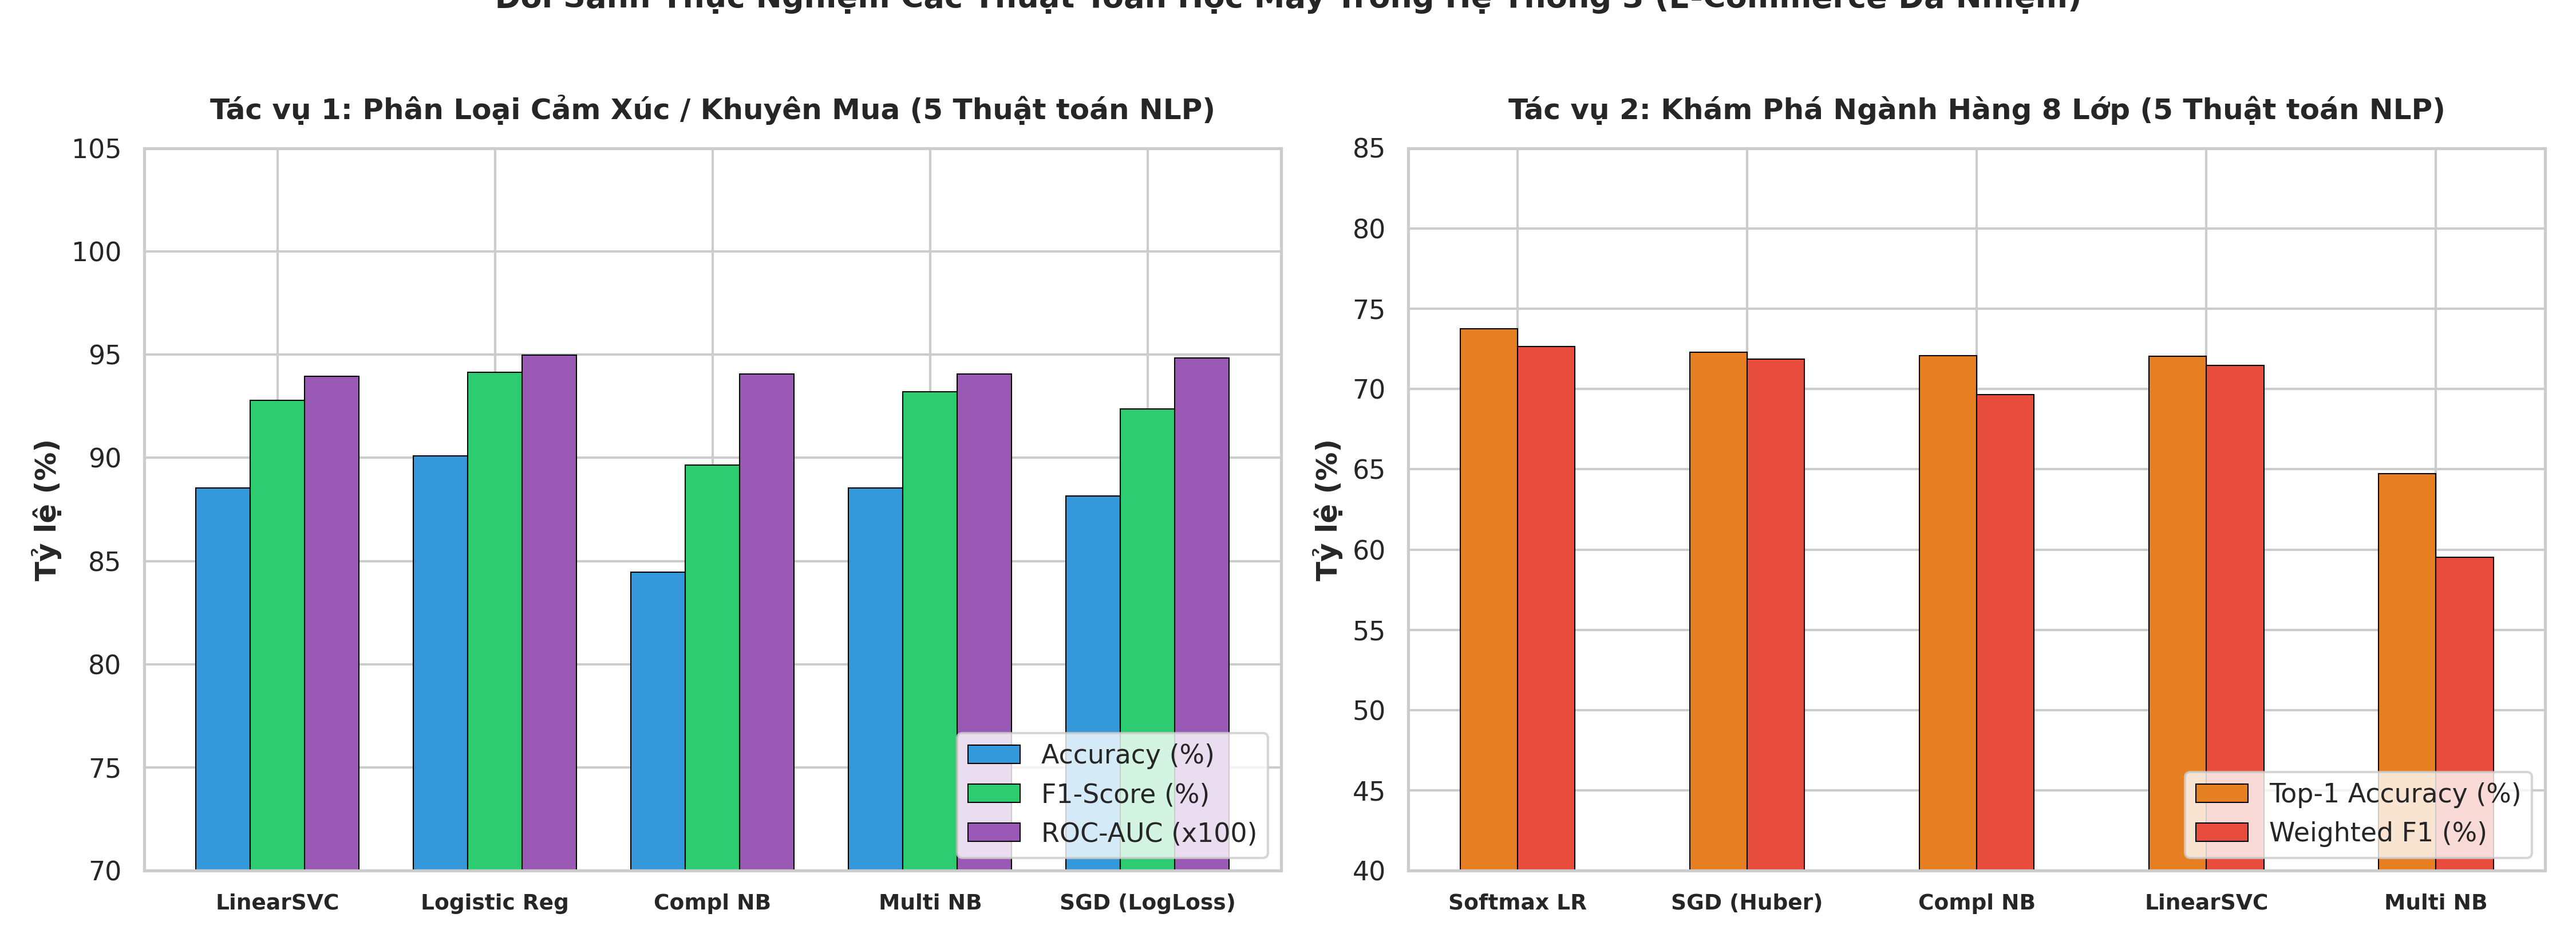
\includegraphics[width=0.95\textwidth]{images/fig04_ecom_model_comparison.png}
\caption{Đối sánh thực nghiệm các thuật toán học máy trong Hệ thống 3 trên cả hai tác vụ Cảm xúc và Ngành hàng}
\label{fig:ecom_model_benchmark_fig}
\end{figure}

\begin{figure}[H]
\centering
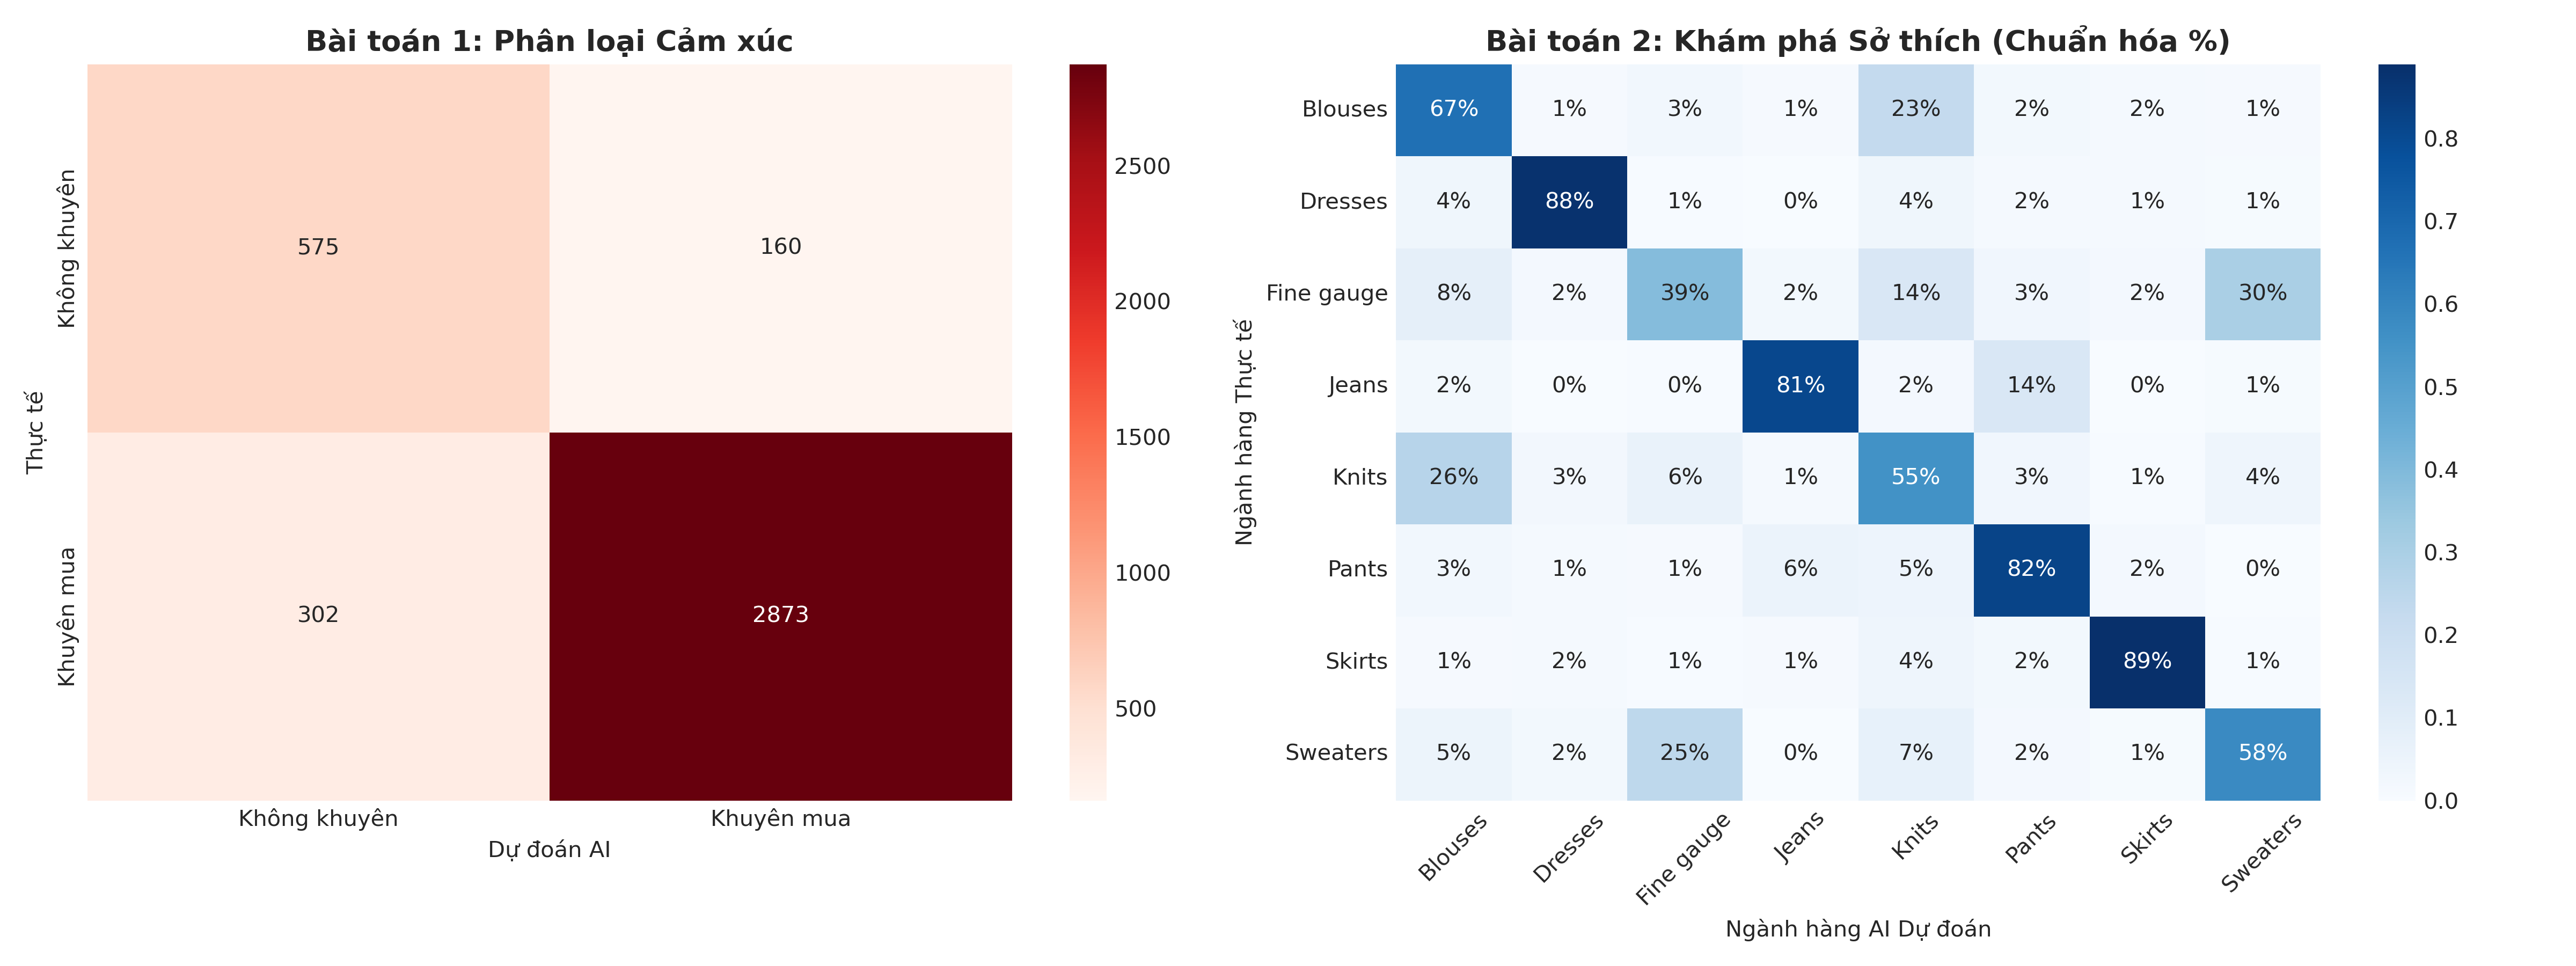
\includegraphics[width=0.85\textwidth]{images/fig02_dual_confusion_matrix.png}
\caption{Ma trận nhầm lẫn kép thể hiện hiệu năng phân loại của cả hai tác vụ Cảm xúc và Ngành hàng}
\label{fig:ecom_dual_cm_plot}
\end{figure}

\subsection{Phân tích Trọng số Từ khóa Then chốt (Key Drivers)}
Hình~\ref{fig:ecom_keywords_chart} trực quan hóa các hệ số hồi quy lớn nhất của mô hình. Các từ khóa mang trọng số dương mạnh nhất (thúc đẩy dự đoán Khuyên mua) bao gồm: \textit{love, perfect, comfortable, flattering, great, beautiful, soft}. Ngược lại, các từ mang trọng số âm lớn nhất (báo hiệu Thất vọng) gồm có: \textit{returned, disappointed, cheap, poor, scratchy, huge, horrible, thin}.

\begin{figure}[H]
\centering
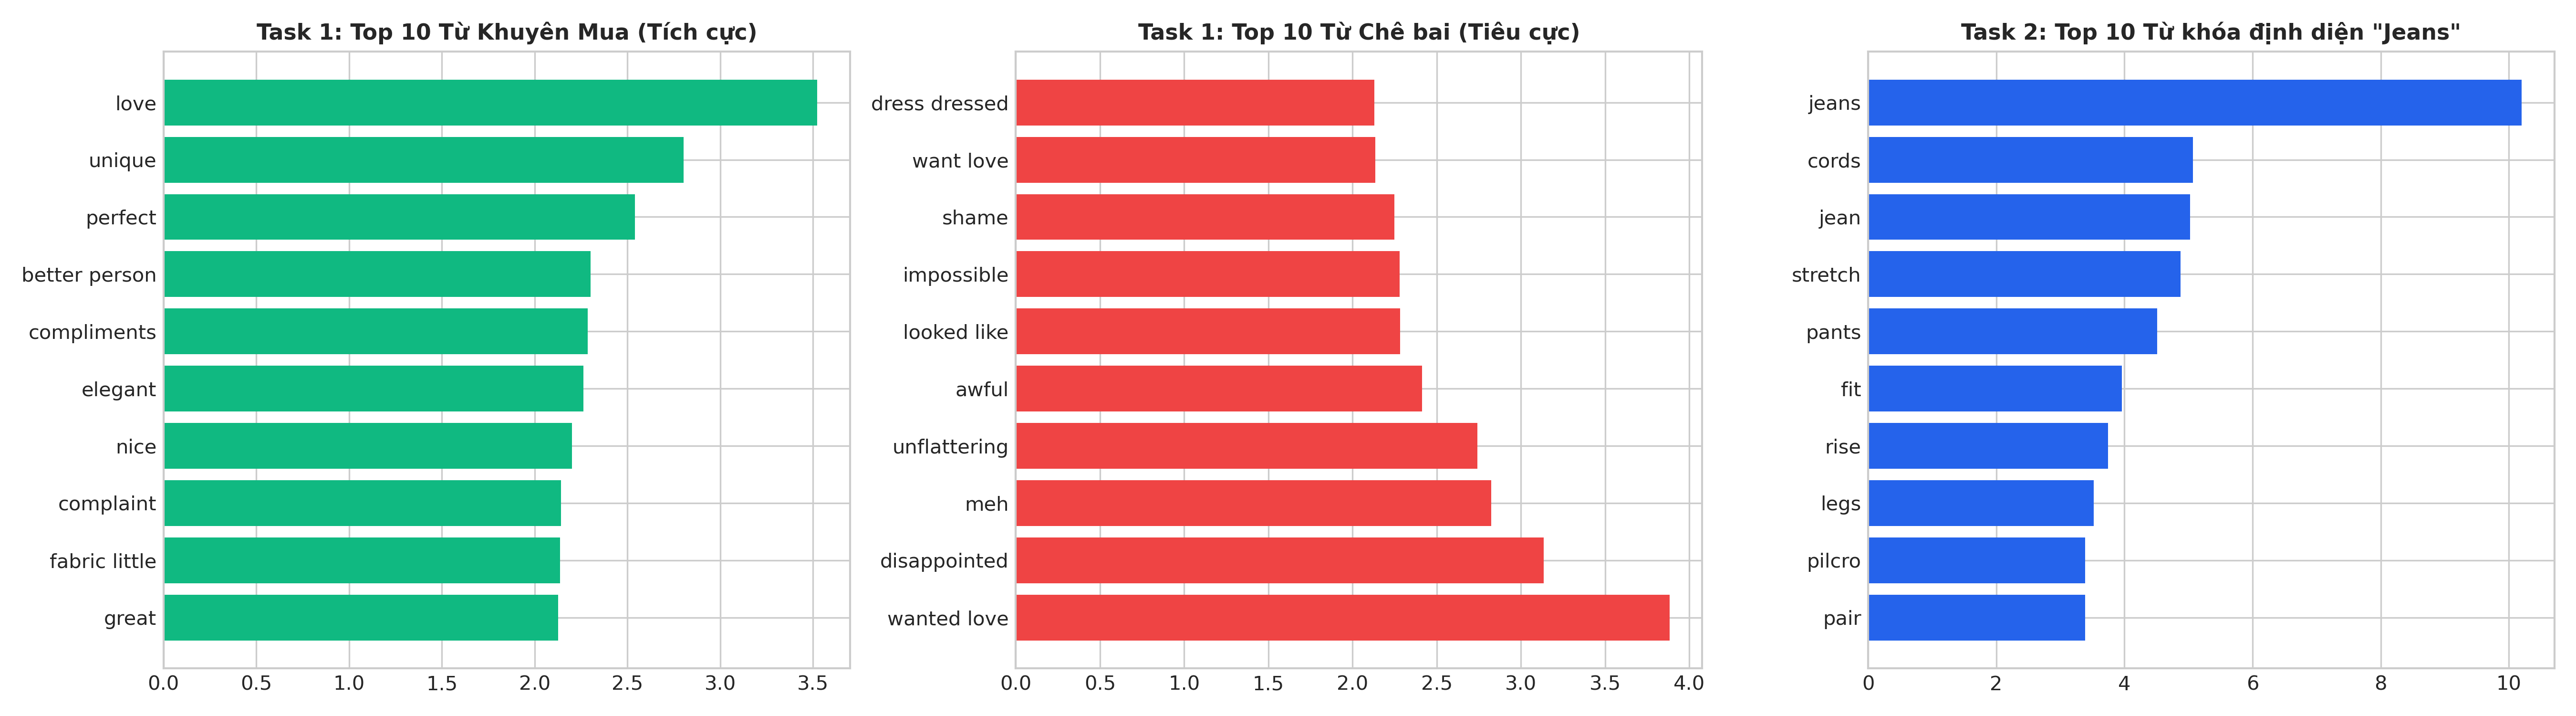
\includegraphics[width=0.85\textwidth]{images/fig03_keyword_analysis.png}
\caption{Biểu đồ phân tích trọng số từ khóa then chốt thúc đẩy cảm xúc tích cực và tiêu cực}
\label{fig:ecom_keywords_chart}
\end{figure}

\section{Tầng Tự Động Hóa Chăm Sóc Khách Hàng (CRM Automation)}
Hệ thống kết nối trực tiếp phân tích NLP với các kịch bản vận hành kinh doanh:
\begin{itemize}[leftmargin=2em]
    \item \textbf{Trích xuất Tín hiệu Cảm xúc Then chốt:} Giao diện tự động phát hiện và làm nổi bật các từ khóa cảm xúc trọng tâm trong bài đánh giá.
    \item \textbf{Kịch bản Khiếu nại \& Phục hồi Khách hàng (Churn Prevention):}
    Khi mô hình phân loại là Thất vọng (Lớp 0):
    \begin{itemize}
        \item Hệ thống nâng mức ưu tiên lên mức Khẩn cấp.
        \item Tự động gửi email xin lỗi kèm đường link tạo đơn đổi size / hoàn hàng miễn phí trong 7 ngày.
        \item Xuất mã Voucher ưu đãi 15\% (\texttt{CARE15}) áp dụng cho đơn hàng kế tiếp để bù đắp trải nghiệm.
        \item Phát cảnh báo tự động gửi tới Trưởng bộ phận Đảm bảo Chất lượng (QC) của ngành hàng tương ứng (ví dụ ngành hàng Dresses) để kiểm tra lỗi lô vải hoặc form cắt may.
    \end{itemize}
    \item \textbf{Kịch bản Khách hàng Thân thiết (Loyalty \& Cross-sell):}
    Khi mô hình phân loại là Hài lòng (Lớp 1):
    \begin{itemize}
        \item Gửi lời mời khách hàng tham gia chương trình VIP Member và tặng 50 điểm thưởng khi đăng ảnh trải nghiệm sản phẩm.
        \item Kích hoạt thuật toán Recommender System gợi ý bán chéo các phụ kiện thời trang phối đồ phù hợp với danh mục ngành hàng vừa nhận diện (ví dụ phối áo khoác ngoài cho Váy liền).
    \end{itemize}
\end{itemize}

% =========================================================================
% CHƯƠNG 5: SO SÁNH CHUYÊN SÂU BA HỆ THỐNG THÔNG MINH
% =========================================================================
\chapter{So Sánh Chuyên Sâu Ba Hệ Thống Thông Minh}

\section{Bảng So Sánh Đa Chiều Toàn Diện}

\begin{table}[H]
\centering
\scriptsize
\caption{Bảng so sánh chuyên sâu ba hệ thống thông minh theo các trục tiêu chí kỹ thuật}
\label{tab:deep_comparison_chapter5}
\begin{tabularx}{\textwidth}{lXXX}
\toprule
\textbf{Tiêu chí So sánh} & \textbf{Hệ thống 1: Tiểu đường} & \textbf{Hệ thống 2: Giá nhà} & \textbf{Hệ thống 3: E-Commerce} \\
\midrule
\textbf{Miền nghiệp vụ} & Y sinh học lâm sàng & Kinh tế bất động sản đô thị & Bán lẻ trực tuyến \& CRM \\
\textbf{Kiểu bài toán ML} & Phân loại nhị phân & Hồi quy giá trị liên tục & Học đa nhiệm (Nhị phân + 8 lớp) \\
\textbf{Bản chất dữ liệu} & Bảng số học cấu trúc cao & Bảng số học + Phân cấp không gian & Văn bản chuỗi tự do (NLP) \\
\textbf{Số quan sát} & 95,155 mẫu sau làm sạch & 144,995 mẫu sau làm sạch & 19,550 mẫu sau làm sạch \\
\textbf{Số chiều đặc trưng} & 14 chiều (Vector đậm đặc) & 13 chiều (Vector đậm đặc) & 4,000 chiều (Ma trận siêu thưa) \\
\textbf{Hiện tượng dữ liệu} & Mất cân bằng nhãn 10.2:1 & Lệch phải sau làm sạch (Skew +3.15) & Mất cân bằng 82:18, văn bản ngắn \\
\textbf{Phép biến đổi chính} & Z-Score, One-Hot, Tích số tương tác & Log-Transform, Target Encoding Bayes & Regex Clean, N-gram TF-IDF Sublinear \\
\textbf{Mô hình tối ưu} & HistGradientBoosting & HistGradientBoosting Tuned & LinearSVC Balanced + Logistic Reg \\
\textbf{Độ đo đánh giá} & ROC-AUC, Recall, F1-Score & $R^2$ Log/Raw, MAE, Median Error & ROC-AUC, F1-Score, Macro Accuracy \\
\textbf{Tầng Ra Quyết Định} & Đánh giá nguy cơ, phác đồ lối sống & Phân khúc thị trường, dải giá niêm yết & Trích xuất từ khóa, CRM hoàn tiền/Upsell \\
\textbf{Kích thước tệp model} & $\approx 380\text{ KB}$ & $\approx 5.2\text{ MB}$ & $\approx 1.8\text{ MB}$ \\
\textbf{Thời gian suy luận} & $< 2\text{ ms}$ & $< 3\text{ ms}$ & $\approx 15\text{ ms}$ \\
\bottomrule
\end{tabularx}
\end{table}

\section{Trả Lời 8 Câu Hỏi Kiến Trúc Cốt Lõi}

\subsection{Ba bộ dữ liệu khác nhau như thế nào?}
Ba bộ dữ liệu đại diện cho 3 bản chất thông tin hoàn toàn khác nhau:
\begin{itemize}[leftmargin=2em]
    \item \textbf{Dữ liệu Y tế (Diabetes):} Dữ liệu bảng lâm sàng chuẩn hóa cao. Các biến số mang ý nghĩa sinh lý học chặt chẽ và có ngưỡng giá trị sinh học bất biến (ví dụ HbA1c 6.5\% luôn là ngưỡng đái tháo đường dù ở bất kỳ quốc gia nào).
    \item \textbf{Dữ liệu Bất động sản (House Price):} Dữ liệu kinh tế thị trường mang tính tương đối và phụ thuộc sâu sắc vào tọa độ không gian địa lý. Giá trị bất động sản chịu ảnh hưởng phi tuyến mạnh mẽ bởi vị trí bang, thành phố và quy mô công trình.
    \item \textbf{Dữ liệu Đánh giá Khách hàng (E-Commerce):} Dữ liệu văn bản phi cấu trúc, giàu cảm xúc chủ quan, chứa nhiều từ ngữ đời thường, tiếng lóng và biến thiên lớn về độ dài câu văn.
\end{itemize}

\subsection{Biểu diễn dữ liệu khác nhau như thế nào?}
\begin{itemize}[leftmargin=2em]
    \item \textbf{Diabetes:} Biểu diễn dưới dạng \textbf{Vector đậm đặc (Dense Vector) 14 chiều}, trong đó mỗi chiều mang một ý nghĩa đo lường sinh học cụ thể sau khi được chuẩn hóa Z-score.
    \item \textbf{House Price:} Biểu diễn dưới dạng \textbf{Vector đậm đặc 13 chiều} kết hợp các tỷ lệ diện tích không gian và các giá trị kỳ vọng cục bộ sinh ra từ bộ mã hóa mục tiêu (Target Encoding).
    \item \textbf{Customer Behavior:} Biểu diễn dưới dạng \textbf{Vector siêu thưa (Sparse Vector) 4,000 chiều}, trong đó hơn 98\% các phần tử mang giá trị 0, phản ánh sự xuất hiện có trọng số của các n-gram từ vựng.
\end{itemize}

\subsection{Những bước tiền xử lý nào là chung?}
Cả ba hệ thống đều tuân thủ các nguyên tắc kỹ thuật chuẩn mực của khoa học dữ liệu:
\begin{itemize}[leftmargin=2em]
    \item \textbf{Nguyên tắc Phân chia Dữ liệu Nghiêm ngặt:} Phân chia Train/Test Split trước khi áp dụng bất kỳ bước tiền xử lý nào để triệt tiêu nguy cơ rò rỉ dữ liệu (Data Leakage).
    \item \textbf{Nguyên tắc Fit-Transform Độc lập:} Các đối tượng tiền xử lý (gồm \texttt{StandardScaler}, \texttt{TargetEncoder} và \texttt{TfidfVectorizer}) chỉ học thông số từ tập Train, sau đó áp dụng đồng nhất cho tập Test và Production.
    \item \textbf{Đóng gói Trạng thái Tiền xử lý:} Lưu trữ các đối tượng tiền xử lý thành các tệp nhị phân \texttt{.joblib} độc lập để nạp vào bộ nhớ RAM máy chủ API khi khởi động.
\end{itemize}

\subsection{Những bước tiền xử lý nào mang tính riêng biệt?}
\begin{itemize}[leftmargin=2em]
    \item \textbf{Diabetes:} Kỹ nghệ đặc trưng tương tác nhân quả sinh học ($\text{glucose} \times \text{HbA1c}$) và tối ưu hóa ngưỡng quyết định lâm sàng $\theta = 0.32$.
    \item \textbf{House Price:} Biến đổi hàm log tự nhiên cho biến mục tiêu và kỹ thuật làm mượt Bayes đa tầng (Empirical Bayes Target Encoding).
    \item \textbf{Customer Behavior:} Làm sạch văn bản tự nhiên bằng Regex, ghép chuỗi ngữ cảnh tiêu đề và phân tích từ điển n-gram có trọng số TF-IDF nén tần suất.
\end{itemize}

\subsection{Vì sao biểu diễn Target khác nhau?}
Bản chất câu hỏi nghiệp vụ quyết định không gian biến mục tiêu:
\begin{itemize}[leftmargin=2em]
    \item \textbf{Diabetes:} Target là biến nhị phân $y \in \{0, 1\}$ thể hiện trạng thái bệnh lý có hoặc không có bệnh.
    \item \textbf{House Price:} Target là biến định lượng liên tục $y \in \mathbb{R}^+$ đo lường giá trị tiền tệ thực tế.
    \item \textbf{Customer Behavior:} Target là hệ đa nhiệm gồm một biến nhị phân $y_1 \in \{0, 1\}$ (Hài lòng khuyên mua) và một biến định danh danh nghĩa đa lớp $y_2 \in \{1, \dots, 8\}$ (Ngành hàng thời trang).
\end{itemize}

\subsection{Vì sao cần các Metric đánh giá khác nhau?}
\begin{itemize}[leftmargin=2em]
    \item \textbf{Phân loại Y tế:} Sự mất cân bằng nhãn đòi hỏi ưu tiên \textbf{Recall} (hạn chế tối đa bỏ lọt bệnh nhân) và \textbf{ROC-AUC} (đánh giá khả năng phân tách tổng quát không phụ thuộc ngưỡng).
    \item \textbf{Hồi quy Bất động sản:} Cần chỉ số \textbf{$R^2$} để đo lường tỷ lệ phương sai giải thích được, \textbf{MAE} để xác định độ lệch tiền tệ trung bình, và \textbf{Median Error} để loại bỏ tác động của các giao dịch ngoại lai đột biến.
    \item \textbf{Phân loại Văn bản Đa lớp:} Cần \textbf{Macro F1-Score} để đảm bảo mô hình hoạt động chính xác đồng đều trên toàn bộ 8 ngành hàng, tránh việc mô hình chỉ thiên vị lớp có số lượng mẫu áp đảo.
\end{itemize}

\subsection{Hệ thống nào dễ triển khai nhất?}
\textbf{Hệ thống 1 (Dự đoán Tiểu đường)} là hệ thống dễ triển khai nhất. Mô hình có kích thước tệp rất nhỏ ($< 400\text{ KB}$), số trường đầu vào chỉ gồm 8 biến lâm sàng tường minh, tốc độ suy luận dưới 2 mili-giây, cực kỳ lý tưởng để nhúng trực tiếp vào các thiết bị y tế cá nhân hoặc ứng dụng di động theo dõi sức khỏe.

\subsection{Hệ thống nào đòi hỏi tính toán nhiều nhất?}
\textbf{Hệ thống 3 (E-Commerce)} đòi hỏi năng lực tính toán và bộ nhớ lớn nhất. Quá trình phân tích token văn bản, ánh xạ qua ma trận từ điển 4,000 chiều và tính toán song song hai mô hình phân loại (LinearSVC và Softmax 8 lớp) tiêu tốn nhiều tài nguyên CPU hơn đáng kể so với các phép biến đổi số học đơn giản của Hệ thống 1 và 2.

% =========================================================================
% CHƯƠNG 6: KIẾN TRÚC TRIỂN KHAI VÀ GIAO DIỆN SẢN PHẨM
% =========================================================================
\chapter{Kiến Trúc Triển Khai và Hiện Thực Giao Diện Sản Phẩm}

\section{Kiến Trúc Tổng Thể Hệ Thống (System Architecture)}
Hệ thống được thiết kế theo kiến trúc Microservice hướng dịch vụ (Service-Oriented Architecture) gồm 3 tầng khép kín:
\begin{enumerate}
    \item \textbf{Tầng Trình Diễn (Presentation Layer):} Giao diện Web Responsive hiện đại tích hợp bộ giả lập thiết bị di động (Mobile Simulator).
    \item \textbf{Tầng Dịch Vụ API (Backend Service Layer):} Xây dựng trên framework \textbf{FastAPI (Python)}, cung cấp các REST API endpoints chuẩn hóa, xác thực dữ liệu qua Pydantic schemas và tự động sinh tài liệu Swagger UI.
    \item \textbf{Tầng Suy Luận \& Khuyến Nghị (Inference \& Advisory Engine):} Nạp các mô hình đã huấn luyện lên bộ nhớ RAM, thực hiện tiền xử lý, tính toán xác suất và khởi chạy module tư vấn quyết định chuyên gia.
\end{enumerate}

\begin{figure}[H]
\centering
\begin{tikzpicture}[node distance=1.5cm, auto, >=Latex]
    \tikzstyle{client} = [rectangle, draw=black!70, fill=blue!15, text width=6.5cm, text centered, rounded corners=4pt, minimum height=1.1cm, font=\small\bfseries]
    \tikzstyle{api} = [rectangle, draw=black!70, fill=green!15, text width=7.6cm, text centered, rounded corners=4pt, minimum height=1.2cm, font=\small\bfseries]
    \tikzstyle{model} = [rectangle, draw=black!70, fill=orange!15, text width=5.0cm, text centered, rounded corners=4pt, minimum height=1.3cm, font=\small]
    \tikzstyle{advisory} = [rectangle, draw=black!70, fill=purple!15, text width=5.0cm, text centered, rounded corners=4pt, minimum height=1.3cm, font=\small\bfseries]

    \node [client] (web) {Client: Web App / Mobile Viewport Simulator\\{\footnotesize (HTML5, Vanilla CSS, Responsive UI)}};
    \node [api, below of=web, node distance=2.4cm] (fastapi) {FastAPI RESTful API Backend Server\\{\footnotesize (Pydantic Validation + Routing + Swagger UI)}};
    \node [model, below of=fastapi, node distance=2.7cm, xshift=-3.5cm] (inf) {\textbf{Tầng Mô Hình Học Máy}\\(\texttt{model.joblib}, \texttt{preprocessor}\\Pipeline in RAM)};
    \node [advisory, below of=fastapi, node distance=2.7cm, xshift=3.5cm] (adv) {\textbf{Tầng Khuyến Nghị Chuyên Gia}\\(Clinical / Real Estate Market /\\CRM Automation Rules)};

    % Client <-> FastAPI: Parallel separated arrows (No collision)
    \draw [->, thick, >=Latex, draw=blue!80!black] ([xshift=1.5cm]web.south) -- node[right, font=\scriptsize, text=black] {HTTP POST (JSON Request)} ([xshift=1.5cm]fastapi.north);
    \draw [->, thick, >=Latex, draw=green!70!black] ([xshift=-1.5cm]fastapi.north) -- node[left, font=\scriptsize, text=black] {JSON Response (Dự báo + Tư vấn)} ([xshift=-1.5cm]web.south);

    % FastAPI -> Model -> Advisory -> FastAPI (Clean loop with clear spacing)
    \draw [->, thick, >=Latex, draw=orange!80!black] ([xshift=-2.2cm]fastapi.south) -- node[left, font=\scriptsize, text=black, align=right] {1. Vector đặc trưng\\(Features Input)} ([xshift=-0.5cm]inf.north);
    \draw [->, thick, >=Latex, draw=purple!80!black] (inf.east) -- node[above, font=\scriptsize, text=black, align=center] {2. Kết quả Dự báo} node[below, font=\scriptsize, text=black, align=center] {\& Xác suất / Giá trị} (adv.west);
    \draw [->, thick, >=Latex, draw=green!60!black] ([xshift=0.5cm]adv.north) -- node[right, font=\scriptsize, text=black, align=left] {3. Kế hoạch Hành động\\\& Tư vấn Chuyên gia} ([xshift=2.2cm]fastapi.south);
\end{tikzpicture}
\caption{Sơ đồ kiến trúc phân tầng và luồng dữ liệu xử lý của hệ thống thông minh}
\label{fig:full_system_arch}
\end{figure}

\section{Hiện Thực Giao Diện Thực Tế Của Ba Hệ Thống}

\subsection{Hệ thống 1: Tiểu đường}
Hình~\ref{fig:ui_sys1_in} minh chứng giao diện tiếp nhận thông số lâm sàng. Điểm nổi bật là thanh \textbf{Động cơ AI (AI Engine)} được tách riêng ở đầu form, cho phép người dùng linh hoạt lựa chọn thuật toán suy luận (HistGradientBoosting hoặc Logistic Regression).

\begin{figure}[H]
\centering
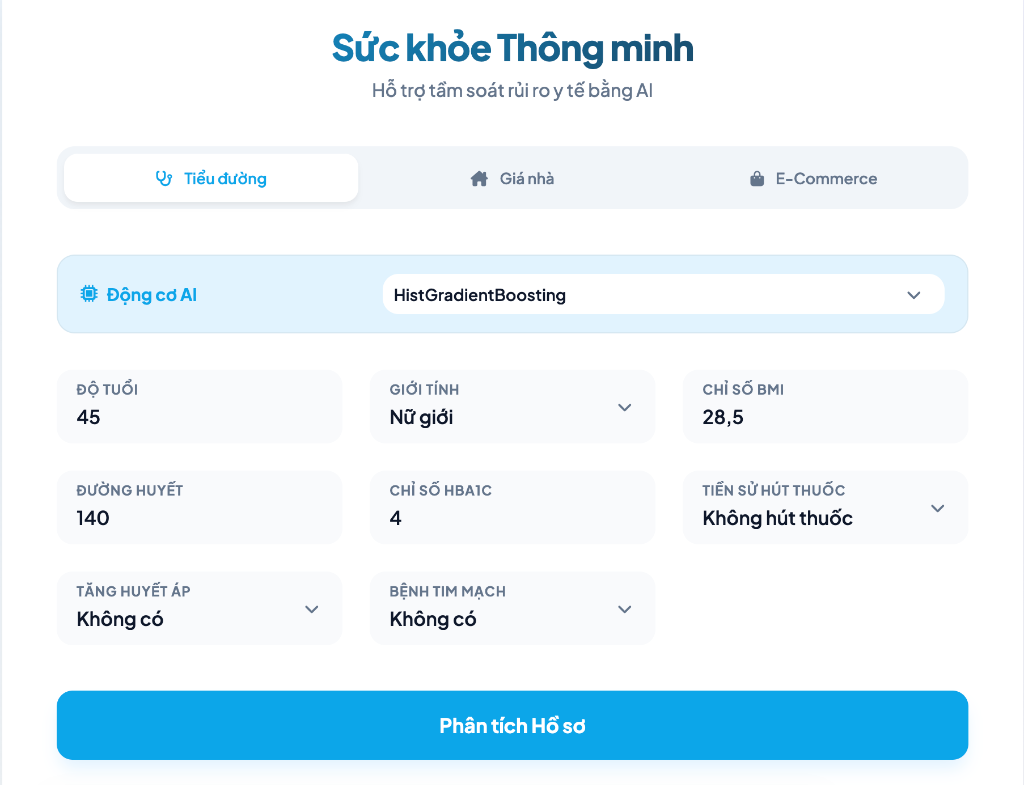
\includegraphics[width=0.85\textwidth]{images/ui_sys1_input.png}
\caption{Giao diện tiếp nhận hồ sơ lâm sàng và bộ chọn Động cơ AI (Hệ thống 1)}
\label{fig:ui_sys1_in}
\end{figure}

Hình~\ref{fig:ui_sys1_flags} và Hình~\ref{fig:ui_sys1_advice} thể hiện Tầng Ra Quyết Định Y Khoa. Dù kết quả dự báo chung là An toàn (Xác suất 1.3\%), hệ thống vẫn tự động gắn nhãn cảnh báo \textbf{Báo động (Đỏ)} cho đường huyết $140\text{ mg/dL}$ và \textbf{Lưu ý (Vàng)} cho thể trạng thừa cân BMI 28.5, đồng thời xuất hướng dẫn chế độ ăn và kế hoạch khám tầm soát tiếp theo.

\begin{figure}[H]
\centering
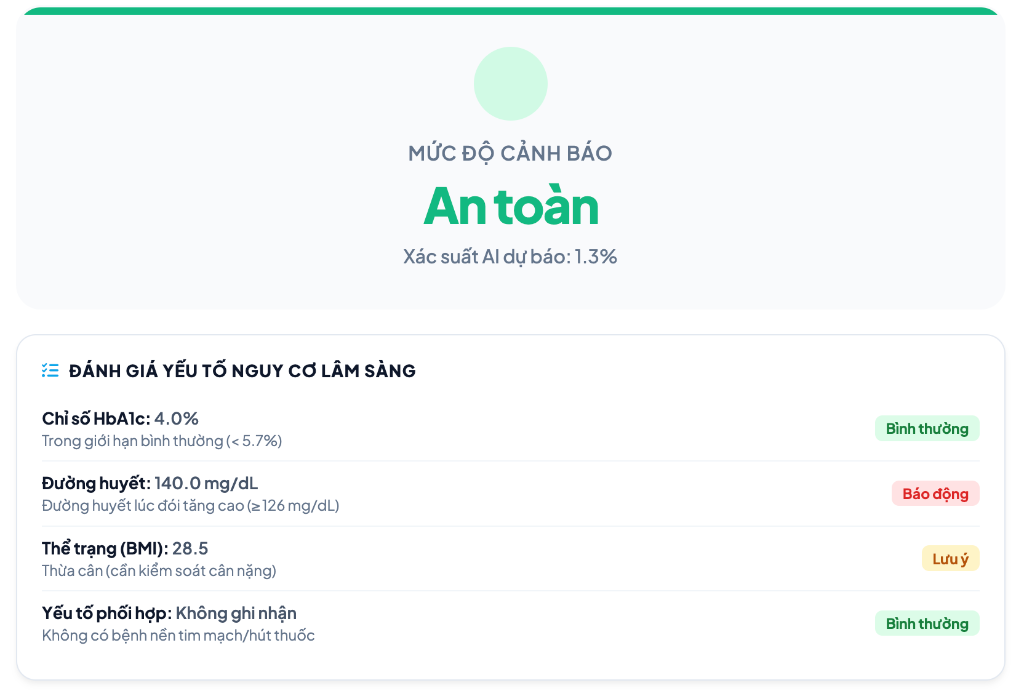
\includegraphics[width=0.85\textwidth]{images/ui_sys1_risk_eval.png}
\caption{Thẻ mức độ cảnh báo và Bảng đánh giá yếu tố nguy cơ lâm sàng gắn nhãn màu (Hệ thống 1)}
\label{fig:ui_sys1_flags}
\end{figure}

\begin{figure}[H]
\centering
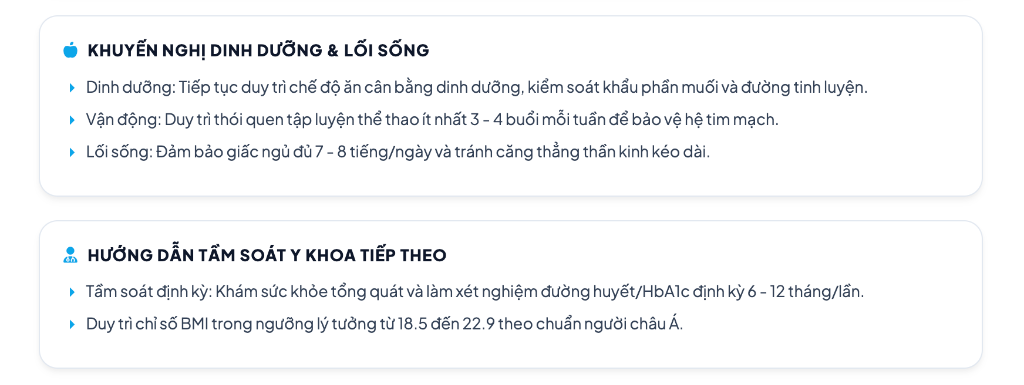
\includegraphics[width=0.85\textwidth]{images/ui_sys1_advisory.png}
\caption{Thẻ khuyến nghị dinh dưỡng, lối sống và kế hoạch tầm soát y khoa (Hệ thống 1)}
\label{fig:ui_sys1_advice}
\end{figure}

\subsection{Hệ thống 2: Định giá Bất động sản}
Hình~\ref{fig:ui_sys2_in} minh chứng form nhập liệu thông tin căn nhà gồm diện tích sàn, diện tích đất, số phòng cùng combobox chọn Bang và Thành phố chuẩn hóa.

\begin{figure}[H]
\centering
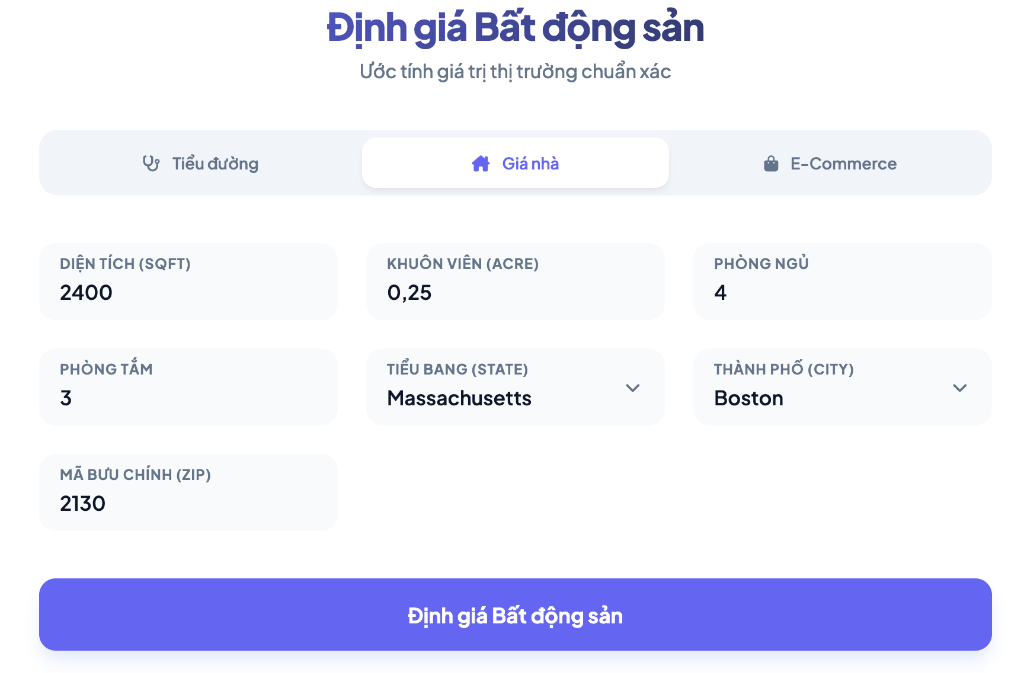
\includegraphics[width=0.85\textwidth]{images/ui_sys2_input.png}
\caption{Giao diện Form nhập liệu đặc trưng căn nhà và định vị địa lý (Hệ thống 2)}
\label{fig:ui_sys2_in}
\end{figure}

Hình~\ref{fig:ui_sys2_strat} minh họa Tầng Tư vấn Chiến lược Bất động sản. Với căn nhà 2,400 sqft tại Boston, hệ thống định giá \$1,349,477 (đơn giá \$562.3/sqft), phân loại thuộc Phân khúc Cao cấp và chỉ ra mức giá này cao hơn 57.6\% so với mặt bằng chung tại Boston. Đồng thời, tư vấn chiến lược đề xuất khoảng giá chào bán khuyến nghị (\$1,308,993 -- \$1,403,457) và vùng giá đàm phán hợp lý (\$1,255,014) cho bên mua.

\begin{figure}[H]
\centering
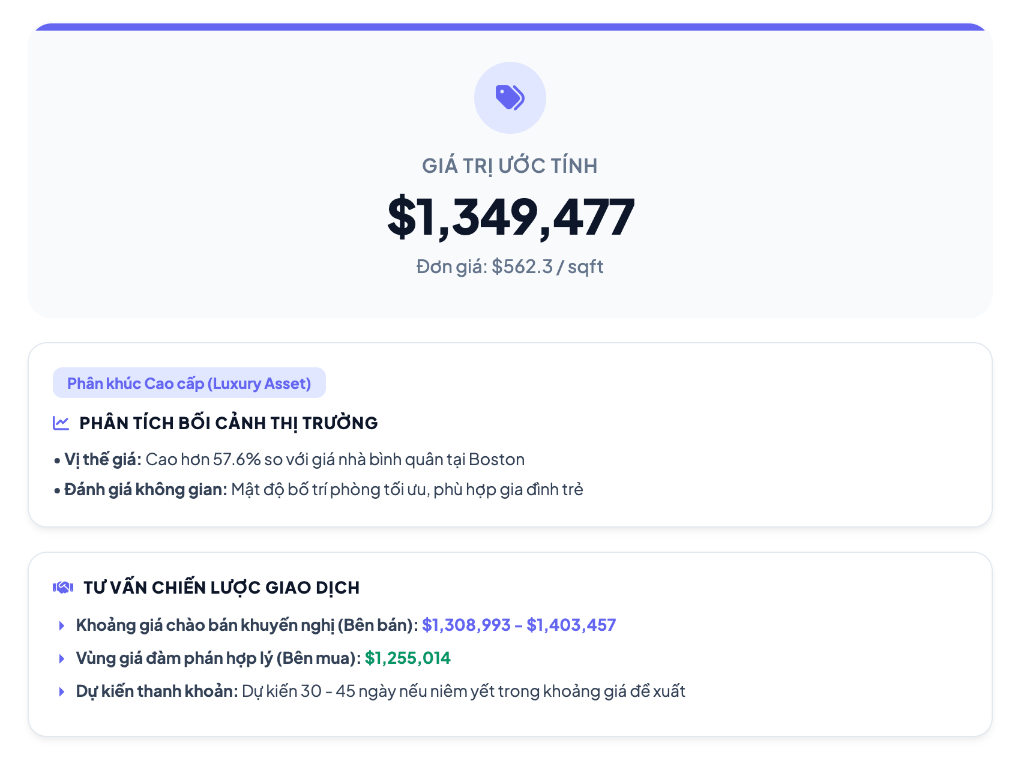
\includegraphics[width=0.85\textwidth]{images/ui_sys2_advisory.png}
\caption{Kết quả định giá kèm Phân tích thị trường và Tư vấn chiến lược giao dịch (Hệ thống 2)}
\label{fig:ui_sys2_strat}
\end{figure}

\subsection{Hệ thống 3: E-Commerce Đa nhiệm}
Hình~\ref{fig:ui_sys3_in} thể hiện giao diện tiếp nhận văn bản đánh giá tự nhiên của khách hàng bằng tiếng Anh kèm nút bấm ``Đọc hiểu Ngôn ngữ''.

\begin{figure}[H]
\centering

\includegraphics[width=0.85\textwidth]{images/ui_sys3_input.png}
\caption{Giao diện tiếp nhận văn bản đánh giá của khách hàng (Hệ thống 3)}
\label{fig:ui_sys3_in}
\end{figure}

Hình~\ref{fig:ui_sys3_crm} minh họa kết quả phân tích kép đồng thời: hệ thống vừa xác định mức độ cảm xúc là \textbf{Hài lòng (Khuyên mua)}, vừa nhận diện danh mục ngành hàng là \textbf{Knits (Đồ dệt kim)} có kèm phần dịch thuật tiếng Việt. Thẻ Tín hiệu Cảm xúc trích xuất chính xác từ khóa cốt lõi (\texttt{recommend}), và Tầng CRM Automation đề xuất ngay kịch bản mời tham gia VIP Member nhận 50 điểm thưởng cùng chiến lược bán chéo phụ kiện phối đồ tương thích.

\begin{figure}[H]
\centering
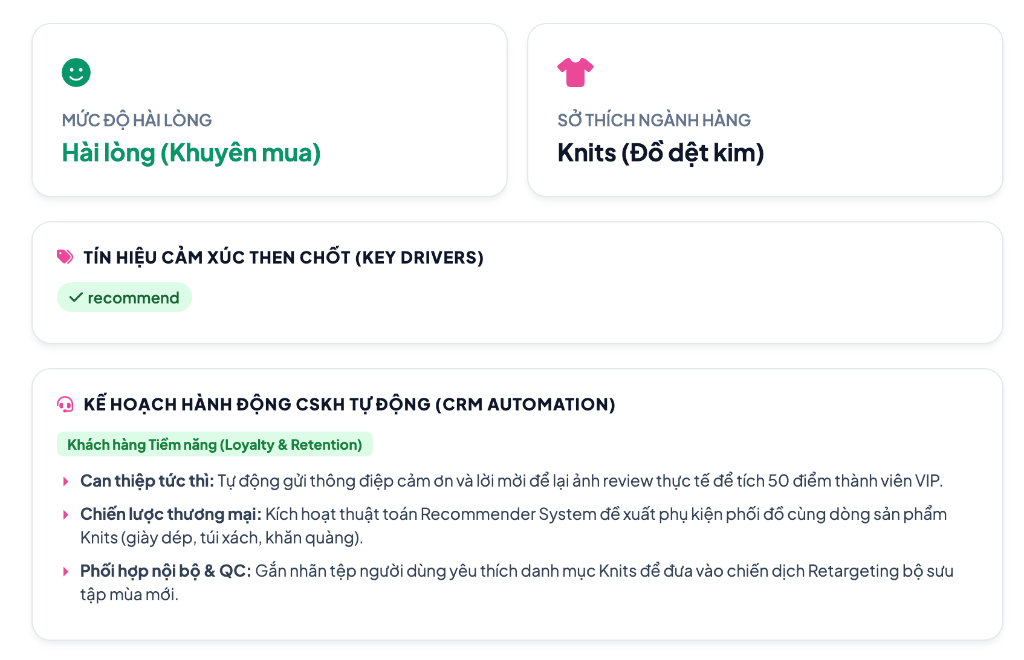
\includegraphics[width=0.85\textwidth]{images/ui_sys3_advisory.png}
\caption{Kết quả phân tích kép kèm Kế hoạch CRM tự động hóa (Hệ thống 3)}
\label{fig:ui_sys3_crm}
\end{figure}

% =========================================================================
% CHƯƠNG 7: THẢO LUẬN, KHẢ NĂNG TÁI LẬP VÀ HẠN CHẾ
% =========================================================================
\chapter{Thảo Luận Chuyên Môn, Khả Năng Tái Lập và Hạn Chế}

\section{Khả Năng Tái Lập Thực Nghiệm (Reproducibility Audit)}
Để đảm bảo chuẩn mực khoa học, toàn bộ quy trình thực nghiệm được thiết kế có khả năng tái lập 100\%:
\begin{itemize}[leftmargin=2em]
    \item \textbf{Kho Lưu Trữ Mã Nguồn Dự Án (GitHub):}\\Toàn bộ mã nguồn, dữ liệu thực nghiệm, pipeline xử lý và giao diện ứng dụng được lưu trữ công khai tại kho lưu trữ:\\\href{https://github.com/phamtu2x5/INTELLIGENT-SYSTEM-DEVELOPMENT}{\texttt{INTELLIGENT-SYSTEM-DEVELOPMENT}}.
    \item \textbf{Liên Kết Trực Tiếp Tới Notebooks Của Ba Hệ Thống:}
    \begin{itemize}
        \item \textit{Hệ thống 1 (Tiểu đường):} \href{https://github.com/phamtu2x5/INTELLIGENT-SYSTEM-DEVELOPMENT/blob/main/src/Assigment%2002/diabetes/notebook/01_diabetes_pipeline.ipynb}{\texttt{01\_diabetes\_pipeline.ipynb}}
        \item \textit{Hệ thống 2 (Bất động sản):} \href{https://github.com/phamtu2x5/INTELLIGENT-SYSTEM-DEVELOPMENT/blob/main/src/Assigment%2002/house_price/notebook/01_house_price_pipeline.ipynb}{\texttt{01\_house\_price\_pipeline.ipynb}}
        \item \textit{Hệ thống 3 (E-Commerce):} \href{https://github.com/phamtu2x5/INTELLIGENT-SYSTEM-DEVELOPMENT/blob/main/src/Assigment%2002/customer_behavior/notebook/01_customer_behavior_pipeline.ipynb}{\texttt{01\_customer\_behavior\_pipeline.ipynb}}
    \end{itemize}
    \item \textbf{Cố định Hạt giống Ngẫu nhiên:} Toàn bộ các thao tác xáo trộn dữ liệu, chia tập Train/Test, khởi tạo trọng số mô hình đều được cố định tại \texttt{random\_state = 42}.
    \item \textbf{Môi trường Thực thi Đồng nhất:} Quản lý thư viện phụ thuộc thông qua môi trường ảo Python 3.12 với các phiên bản chính xác: \texttt{scikit-learn==1.4.2}, \texttt{fastapi==0.110.0}, \texttt{uvicorn==0.29.0}, \texttt{pandas==2.2.1}, \texttt{numpy==1.26.4}.
    \item \textbf{Đóng gói Mô hình:} Toàn bộ các mô hình và đối tượng biến đổi dữ liệu được lưu trữ nhị phân tại thư mục \texttt{model/}, sẵn sàng cho việc tái kiểm chuẩn độc lập bất kỳ lúc nào.
\end{itemize}

\section{Thảo Luận Về Những Hạn Chế Của Hệ Thống}
Mặc dù đạt được những kết quả thực nghiệm rất khả quan, báo cáo thẳng thắn chỉ ra các giới hạn nội tại cần tiếp tục hoàn thiện:
\begin{enumerate}[leftmargin=2em]
    \item \textbf{Hạn chế Hệ thống Tiểu đường (Y tế):} Dữ liệu thu thập là dữ liệu cắt ngang (Cross-sectional Data) tại một thời điểm, chưa theo dõi được biến động liên tục theo chuỗi thời gian (như dữ liệu từ máy đo đường huyết liên tục CGM). Dự đoán của mô hình mang tính chất sàng lọc nguy cơ ban đầu và tuyệt đối không thay thế cho chẩn đoán chuyên sâu của bác sĩ y khoa.
    \item \textbf{Hạn chế Hệ thống Bất động sản:} Mô hình hiện tại chưa tích hợp dữ liệu hình ảnh thực tế của căn nhà (Visual Features) và thông tin hướng phong thủy, chất lượng nội thất cũng như tính pháp lý của bất động sản. Đây là những nguyên nhân chính khiến hệ số giải thích $R^2$ còn khoảng trống $18\%$ biến thiên chưa thể mô hình hóa.
    \item \textbf{Hạn chế Hệ thống E-Commerce (NLP):} Phương pháp biểu diễn TF-IDF là mô hình túi từ (Bag-of-Words) tuy có tốc độ suy luận cực nhanh nhưng chưa hiểu sâu được các cấu trúc ngữ nghĩa phức tạp như câu mỉa mai (Sarcasm), châm biếm hoặc ngữ cảnh phủ định đa tầng. Hướng phát triển trong tương lai là tích hợp các mô hình ngôn ngữ lớn (LLM / Transformers như RoBERTa hoặc DeBERTa).
\end{enumerate}

% =========================================================================
% KẾT LUẬN
% =========================================================================
\chapter*{Kết Luận}
\addcontentsline{toc}{chapter}{Kết Luận}

Báo cáo Assignment 02 đã hoàn thành các nội dung nghiên cứu và triển khai thực nghiệm theo yêu cầu của học phần \textbf{Phát triển các Hệ thống Thông minh}:

\begin{enumerate}[leftmargin=2em]
    \item \textbf{Khảo sát và áp dụng các kỹ thuật biểu diễn dữ liệu đa dạng:} Đã phân tích cơ sở lý thuyết và áp dụng các phương pháp biểu diễn số học phù hợp với từng miền dữ liệu cụ thể: Vector đặc trưng chuẩn hóa cho dữ liệu bảng y tế lâm sàng; Mã hóa không gian địa lý làm mượt Bayes (Target Encoding) cho dữ liệu bất động sản; và Không gian vector n-gram TF-IDF cho văn bản tự nhiên.
    \item \textbf{Quy trình phân tích dữ liệu và đối sánh mô hình:} Tiến hành phân tích khám phá (EDA), tiền xử lý và làm sạch dữ liệu, khảo sát đối sánh thực nghiệm các thuật toán học máy phổ biến trên các tập dữ liệu thực tế và phân tích ngưỡng quyết định phù hợp cho từng bài toán.
    \item \textbf{Thiết kế hệ thống thông minh theo kiến trúc phân tầng:} Kết hợp mô hình học máy với logic nghiệp vụ để xây dựng quy trình ba tầng: \textit{Tầng Dự đoán (Predictive) $\rightarrow$ Tầng Giải thích (Explainable) $\rightarrow$ Tầng Hỗ trợ Quyết định (Advisory Layer)}.
    \item \textbf{Đóng gói và hiện thực hóa giao diện ứng dụng:} Triển khai dịch vụ backend FastAPI RESTful API kết hợp giao diện Web ứng dụng có tích hợp khung hiển thị giả lập thiết bị di động, minh họa trực quan khả năng tương tác của người dùng với hệ thống.
\end{enumerate}

Quá trình thực hiện bài tập lớn giúp sinh viên củng cố kiến thức lý thuyết về học máy, rèn luyện phương pháp luận thực nghiệm và tích lũy thêm kỹ năng kỹ nghệ phần mềm phục vụ việc xây dựng các ứng dụng thông minh trong thực tiễn.

\end{document}
